% !TeX program = pdflatex
\documentclass[11pt, letterpaper,oneside]{memoir}
\usepackage[margin=1in]{geometry}
\usepackage[utf8]{inputenc}
\usepackage[USenglish]{babel}
%\usepackage[english]{fancyref}  
\usepackage{graphicx}
\usepackage{tabularx}
\usepackage{booktabs}
\usepackage{pdfpages}
\usepackage{float}
\usepackage{stix}
\usepackage{url}
\usepackage{eso-pic}
\usepackage{hyperref}
\usepackage{footnotebackref}
\usepackage[inline]{enumitem}
\usepackage{amsmath}
\usepackage{amssymb}
\usepackage{amsthm}
\usepackage{commath}
\usepackage{dirtree}
\usepackage{caption}
\usepackage{subcaption}
%\usepackage[newfloat]{minted}
\usepackage{inconsolata}
\usepackage{appendix}
\usepackage{xparse}
\usepackage{multirow}
\usepackage{tikz}
\usepackage{colortbl}
\usepackage[disable]{todonotes}
\usepackage{pifont}
\usepackage{placeins}
\usepackage[font=small,labelfont=bf,tableposition=top]{caption}
\usepackage{booktabs,tabularx}

\usepackage{relsize,etoolbox}
\AtBeginEnvironment{quote}{\small}

%\usepackage{draftwatermark}
%\SetWatermarkText{\sffamily RESTRICTED COPY}
%\SetWatermarkScale{0.1}

\usepackage{tablefootnote}
\usepackage[acronym,shortcuts]{glossaries}

\usepackage[numbers,sort&compress]{natbib}
\setsecnumdepth{subsection}
\settocdepth{subsection}
\numberwithin{equation}{section}

\usepackage[separate-uncertainty = true,multi-part-units=single]{siunitx}
%\usepackage{marvosym}
\sisetup{load-configurations = abbreviations}

\definecolor{dblue}{HTML}{145680}
\definecolor{dred}{HTML}{801414}
\definecolor{dgreen}{HTML}{148014}
\definecolor{bgcode}{rgb}{0.95,0.95,0.95}
\hypersetup{colorlinks = true,
			citecolor=dgreen,
			linkcolor=dblue,
			urlcolor=dred}

\bibliographystyle{unsrtnat}

%\AddToShipoutPicture*{%
%	\AtPageLowerLeft{\includegraphics[width=0.3\paperwidth,keepaspectratio,trim={{0.3\paperwidth} {0.2\paperwidth} 0 0},clip]{assets/navstar.pdf}}%
%}

\nonzeroparskip
\setfloatadjustment{marginfigure}{\flushleftright}
\setlength{\parindent}{0em}

%% Table IDs

\newcounter{IDnumbers}
\newcommand\IDnumber{\stepcounter{IDnumbers}\arabic{IDnumbers}}
\preto\tabular{\setcounter{IDnumbers}{0}}

%% Assign commands to dings

\newcommand{\cmark}{\ding{51}}
\newcommand{\xmark}{\ding{55}}

%% Theorem environments

\newtheorem{problem}{Problem}%[section]
\newtheorem{proposition}{Proposition}%[section]
\newtheorem{theorem}{Theorem}%[section]
\newtheorem{fact}{Fact}%[section]
\newtheorem{corollary}{Corollary}[theorem]
\newtheorem{lemma}[theorem]{Lemma}

\theoremstyle{definition}
\newtheorem{remark}{Remark}%[section]

%% Document number

\newcommand\docno{ISS/USLI-PDR}

%% Restriction notice
\newcommand\restrictiontype{UNLIMITED DISTRIBUTION}
\newcommand\restrictiontext{%
	\footnotesize {\bfseries \restrictiontype \ NOTICE}
	
	This report contains sensitive information that is to be used in a restrictive manner and has been issued as a Draft Handbook for early dissemination of its content to a limited audience. As a courtesy to the author and those involved in its publication, it should not be distributed until after any imposed restrictions have been relieved.}
\newcommand\restrictionheadertext{%
	{\bfseries RESTRICTED}
}
\newcommand\restrictionnotice{%
	\begin{tikzpicture}[remember picture,overlay]
	\node[anchor=south,yshift=10pt] at (current page.south) {\fbox{\parbox{\dimexpr\textwidth-\fboxsep-\fboxrule\relax}{\restrictiontext}}};
	\end{tikzpicture}%
}
\newcommand\restrictionheader{%
	\begin{tikzpicture}[remember picture,overlay]
	\node[anchor=north,yshift=-20pt] at (current page.north) {\parbox{\dimexpr\textwidth-\fboxsep-\fboxrule\relax}{\restrictionheadertext}};
	\end{tikzpicture}%
}

%% Epigraph

\epigraphfontsize{\small\itshape}
\setlength\epigraphwidth{11cm}
\setlength\epigraphrule{0pt}

%% Units

\DeclareSIUnit\feet{ft}
\DeclareSIUnit\knot{kt}
\DeclareSIUnit\mile{mi}
\DeclareSIUnit\inch{in}
\DeclareSIUnit\pound{lb}
\DeclareSIUnit\poundm{lbm}
\DeclareSIUnit\poundf{lbf}
\DeclareSIUnit\caliber{cal.}
\DeclareSIUnit\fahrenheit{\degree F}

\makeglossaries

\newacronym{tsg}{TSG}{Trajectory Shaping Guidance}
\newacronym{cm}{CM}{Center of Mass}
\newacronym{cfd}{CFD}{Computational Fluid Dynamics}
\newacronym{iss}{ISS}{Illinois Space Society}
\newacronym{pdr}{PDR}{Preliminary Design Review}
\newacronym{cdr}{CDR}{Critical Design Review}
\newacronym{fmea}{FMEA}{Failure Modes and Effects Analysis}
\newacronym{eia}{EIA}{Environmental Impact Assessment}
\newacronym{conops}{CONOPS}{Concept of Operations}
\newacronym{pha}{PHA}{Personnel Hazard Analysis}
\newacronym{zoh}{ZOH}{Zero-order Hold}
\newacronym{moi}{MoI}{Moment of Inertia}
\newacronym{toi}{ToI}{Tensor of Inertia}
\newacronym{lqr}{LQR}{Linear Quadratic Regulator}
\newacronym{mimo}{MIMO}{Multiple Input Multiple Output}
\newacronym{siso}{SISO}{Single Input Single Output}
\newacronym{rms}{RMS}{Root Mean Square}
\newacronym{vtg}{VTG}{Virtual Target Guidance}
\newacronym{aiz}{AIZ}{Admissible Impact Zone}
\newacronym{iip}{IIP}{Instantaneous Impact Point}
\newacronym{uav}{UAV}{Unmanned Aerial Vehicle}
\newacronym{gdpp}{GDPP}{Generalized Dubins Path Problem}
\newacronym{fts}{FTS}{Flight Termination System}
\newacronym{tvc}{TVC}{Thrust Vector Control}
\newacronym{nfz}{NFZ}{No-Fly Zone}
\newacronym{cv}{CV}{Computer Vision}
\newacronym{rso}{RSO}{Range Safety Officer}
\newacronym{nar}{NAR}{National Association of Rocketry}
\newacronym{tra}{TRA}{Tripoli Rocketry Association}
\newacronym{faa}{FAA}{Federal Aviation Authority}
\newacronym{los}{LOS}{Line of Sight}
\newacronym{vfr}{VFR}{Visual Flight Rules}
\newacronym{imu}{IMU}{Inertial Measurement Unit}
\newacronym{rac}{RAC}{Risk Assessment Code}
\newacronym{uas}{UAS}{Unmanned Aerial System}
\newacronym{fpv}{FPV}{First Person View}
\newacronym{tsa}{TSA}{Transportation Security Administration}
\newacronym{atc}{ATC}{Air Traffic Control}
\newacronym{zenith}{ZENITH}{Zenith Estimation through Numerical Integration and Tractable Heuristics}
\newacronym{gps}{GPS}{Global Positioning System}
\newacronym{mav}{MAV}{Micro Air Vehicle}
\newacronym{emst}{EMST}{Electric Multirotor Sizing Tool}
\newacronym{bemt}{BEMT}{Blade Element Momentum Theory}

% \vec to \mathbf
\usepackage{bm}
\renewcommand{\vec}[1]{\boldsymbol{\mathbf{#1}}}

% dot product
\makeatletter
\newcommand*\dotp{\mathpalette\dotp@{.5}}
\newcommand*\dotp@[2]{\mathbin{\vcenter{\hbox{\scalebox{#2}{$\m@th#1\bullet$}}}}}
\makeatother

% sign function
\DeclareMathOperator{\sign}{sgn}

% maximum column size
\setcounter{MaxMatrixCols}{12}

% variable with reference coordinate and modifier
\NewDocumentCommand{\cvar}{ O{A} o o m }{
	\IfNoValueTF{#3}{
		\IfNoValueTF{#2}{#4_{\text{#1}}}{#4^{(#2)}_{\text{#1}}}
		}{
		\IfNoValueTF{#2}{#4_{\text{#1}}}{#4^{(#2)}_{\text{#1},#3}}}
}

\NewDocumentCommand{\cvarnopar}{ O{A} o o m }{
	\IfNoValueTF{#3}{
		\IfNoValueTF{#2}{#4_{\text{#1}}}{#4^{#2}_{\text{#1}}}
	}{
		\IfNoValueTF{#2}{#4_{\text{#1}}}{#4^{#2}_{\text{#1},#3}}}
}

\NewDocumentCommand{\cvarnosup}{ O{A} o m }{
	\IfNoValueTF{#2}{#3_{\text{#1}}}{#3_{\text{#1},#2}}
}

\NewDocumentCommand{\cvarnosub}{ O{A} o m }{
	\IfNoValueTF{#2}{#3_{\text{#1}}}{#3^{#2}_{\text{#1}}}
}

%\makeevenfoot{headings}{}{\large\textbf{\restrictiontype}}{}
%\makeoddfoot{headings}{}{\large\textbf{\restrictiontype}}{}
%
%\copypagestyle{chapter}{plain}
%\makeevenhead{chapter}{}{\large\textbf{\restrictiontype}}{}
%\makeoddhead{chapter}{}{\large\textbf{\restrictiontype}}{}

\copypagestyle{titlingpage}{plain}

%\makeevenhead{titlingpage}{\Large\textbf{\restrictiontype}}{}{}
%\makeoddhead{titlingpage}{\Large\textbf{\restrictiontype}}{}{}

\makeevenfoot{titlingpage}{}{}{}
\makeoddfoot{titlingpage}{}{}{}

%\makeevenhead{titlingpage}{\Large\textbf{\restrictiontype}}{}{\Large\textbf{COPY NO.}\hspace{0.1cm} \makebox[1.2cm]{\hrulefill}}
%\makeoddhead{titlingpage}{\Large\textbf{\restrictiontype}}{}{\Large\textbf{COPY NO.}\hspace{0.1cm} \makebox[1.2cm]{\hrulefill}}

%\makeevenfoot{titlingpage}{}{\Large\textbf{RESTRICTIONS APPLY}}{}
%\makeoddfoot{titlingpage}{}{\Large\textbf{RESTRICTIONS APPLY}}{}

\begin{document}
	
	% TITLE PAGE
	
	\begin{titlingpage}		
		\raggedleft
		
		\rule{1pt}{\textheight}
		\hspace{0.01\textwidth} % Whitespace between the vertical line and title page text
		\parbox[b]{0.97\textwidth}{ % Paragraph box for holding the title page text, adjust the width to move the title page left or right on the page
			
			{\Large \texttt{\docno}\hfill\texttt{\bfseries DRAFT}}\\[5\baselineskip]
			{\Huge Preliminary Design Review}
			\\
			{\Large In fulfillment of the NASA University Student Launch Initiative requirements}
			\\[3\baselineskip]
			
			\begin{center}
				
\includegraphics[width=0.4\linewidth]{ISSlogo_square}\\
				{\Large University of Illinois at Urbana-Champaign}\\[2\baselineskip]
				{\Large\itshape Illinois Space Society (ISS)}\\[1\baselineskip]
				{\large 104 S Wright Street}\\
				{\large Urbana, Illinois 61801}
			\end{center}
			
			
			\vspace{0.2\textheight} % Whitespace between the title block and the publisher
			\vfill
			
			%{\large\textit{Delft University of Technology, Faculty of Aerospace Engineering}}
			{\noindent \today}\\[\baselineskip] % Publisher and logo
		}
		
	\end{titlingpage}

	\listoftodos

\listoffigures
	
\listoftables

\clearpage

\addcontentsline{toc}{chapter}{Acknowledgement}

\begin{center}
	{\Large\textbf{ACKNOWLEDGEMENT}}\\
	\begin{minipage}[H]{0.75\linewidth}
		\begin{table}[H]
			\begin{tabularx}{\linewidth}{X X l}
				\underline{AREA} & \underline{NAME/FUNCTION} & \underline{SUBTEAM} \\[.75em]
				Parts I, II, VI & H. El-Kebir \newline \textit{Team Lead} & --- \\[1.5em]
				Part III \newline \textit{Vehicle configuration} & G. Petrov \newline \textit{Subteam Lead} & Structures \& Recovery \\[1.5em]
				Part III  \newline \textit{Avionics} & M. Bourla \newline \textit{Subteam Lead} & Avionics \\[1.5em]
				Part III  \newline \textit{Flight simulations} & R. Filipiuk \newline \textit{Subteam Lead} & Flight Dynamics \\[1.5em]
				Part IV \newline \textit{Payload configuration} & K. Tochihara \newline \textit{Project Manager} & Payload \\[1.5em]
				Part IV \newline \textit{Control systems} & A. Yaraneri \newline \textit{Chief Engineer} & Payload \\[1.5em]
				Part V & Z. Essmyer \newline \textit{Ancillary Subteam Lead} & Ancillary
			\end{tabularx}
		\end{table}
	
		\todo[inline, author=HE]{Add administrative and financial officers}
	
		It is requested that any organizations having specific comments in their area of responsibility contact the individual(s) listed above.
	\end{minipage}
\end{center}
\vfill

\newpage

\printglossary[type=\acronymtype]
\addcontentsline{toc}{chapter}{Glossary}

\newpage

\tableofcontents

\chapter{Preface}
	
This document (\texttt{\docno}) serves as the \gls{pdr} for the University of Illinois at Urbana-Champaign University Student Launch Initiative team, \gls{iss}. The content of this report will chiefly focus on the changes since the original proposal, developments in design and underlying justifications, as well as overall prospects and plans towards the \gls{cdr}. In particular, the launch vehicle design is detailed with reference to the pertinent vehicle requirements, providing an overview of its subsystems, interfaces, and manufacturing methods. Safety considerations are addressed through a multitude of simulations, as well as a qualitative \gls{fmea} and \gls{eia}. Following this discussion, the payload requirements and preliminary design of both the airframe and sample retrieval mechanism are presented, culminating in the presentation of a detailed \gls{conops}. The payload--launch vehicle interface as well as the aerial deployment mechanism are discussed, giving rise to a detailed safety analysis. As part of the safety analysis, in addition to a comprehensive \gls{fmea}, a \gls{pha} is presented. Any hazardous activities will be identified as part of this discussion, including any foreseeable contingencies and mitigation procedures. Finally, a project plan is presented, including a project timeline (Gantt chart), bill of materials, list of funding sources and mitigation procedures in case of delays.

This report is composed of six parts, in which each part builds forth upon the previous. These parts are:

\begin{enumerate}[noitemsep, label=\Roman*]
	\item Summary
	\item Changes
	\item Launch Vehicle
	\item Payload
	\item Safety
	\item Project Plan
\end{enumerate}

Each of these parts describes in due detail the developments and rationale behind the launch vehicle and payload design, as well as the overall implementation.

\paragraph{DISCLAIMER:}
While the authors have gone through great lengths to ensure the validity of all data presented in this document, all responsibility is assumed for any inconsistencies presented as part of this work. 

\part{Summary}

\chapter{Executive Summary}

Over the period spanning from proposal submission to \gls{pdr} submission (August--November 2019), the team has made considerable progress in shaping a preliminary vehicle and payload design. Throughout these developments, the project chiefly guided by the the following main goals: safety, feasibility and timeliness. This part will outline the present mission design in relation to these goals, as well as the overall considerations that shaped the leading launch vehicle and payload design.

The launch vehicle is slated to be a single-booster rocket, weighing \SI{10.68}{\kilo\gram} (\SI{23.55}{\poundm}), with a base-to-tip length of \SI{2.41}{\meter} (\SI{7}{\feet} \SI{11}{\inch}). The vehicle caliber is two-fold, as a transition will be utilized so as to attain a wider fairing diameter; the body diameter is \SI{10.16}{\centi\meter} (\SI{4}{\inch}), whereas the fairing diameter is \SI{15.24}{\centi\meter} (\SI{6}{\inch}). In designing the vehicle, a reference altitude of \SI{1.5}{\kilo\meter} (\SI{4921}{\feet}) was aimed at, prompting the appointment of the AeroTech K780R as the motor of choice. This motor has a burn time of \SI{3}{\second}, and produces a total impulse of \SI{2371}{\newton\second} (L-class). The nose cone was chosen to be of tangent ogive shape, with an aspect ratio of 3:1.

% \part{Changes}

\part{Launch Vehicle}

\chapter{Avionics}
\section{Requirements}
The avionics subteam is responsible for completion of a multitude of critical objectives. Specifically, the avionics team was charged with the following: first, the team is responsible for transmitting the deployment signal to the \gls{uav} after receiving clearance from the \gls{rso} so that the rocket’s payload can be ejected. Moreover, the team must know the exact altitude of the rocket through the use of a commercially available altimeter.
Furthermore, the avionics subteam is also responsible for triggering the e-matches which then deploy the main and drogue parachutes
at the correct point in the flight. This is of critical importance to the success of the mission because these signals are used to deploy the parachutes at the correct moment for landing.
In addition to satisfying these team defined objectives, the team must also design the avionics subsystems pursuant to the requirements of the NASA Student Launch competition as specified in the NASA Student Launch handbook. The following section establishes the aforementioned requirements and the team’s efforts to meet them. 

The first critical requirement that falls on the avionics team concerns the barometric altimeter. The rocket must include one commercially available barometric altimeter. The team will include the MPL3115A2 by Xtrinsic, a commercially available altimeter as part of the avionic subsystem for the rocket. 
In addition to the commercially available barometric altimeter mentioned above, there are two other sets of altimeters in two pairs of two altimeters that provide quadruple redundancy. There will be of them is the Stratologger and the other altimeter we are using is the Telemetrum. There will be two sets of both altimeters on the rocket. One of the key components of consideration by the avionic subteam was redundancy in the altimeters. As mentioned earlier it was mentioned that there are four altimeters in addition to the  MPL3115A2. The telemetrums sensor will serve as the backup to the Strotologgers in case of failure. Moreover, each altimeter will act as a fully self contained system with its own source of power (via a battery). Additionally, each altimeter will be armed via a dedicated arming switch that can be accessed from the exterior of the rocket frame. Each arming switch individually locks in its on position once set by a team member; this prevents it from getting disarmed by forces present in flight. Moreover, lithium polymer batteries will be clearly indicated as a fire hazard. All the electronics, including LIPO batteries will be physically segregated from the payload to prevent any damage during the deployment. Additionally, in order to prevent the batteries from being damaged during flight, they will be mounted to a fixed part of the interior of the rocket. 
The telemetrum has an onboard GPS receiver which will be able to keep track of the rocket’s position. This will allow the team to easily recover the rocket. Additionally, the team is strongly considering adding additional GPS sensors to the rocket in order to give the ground receiver, a more accurate estimation of the rocket’s position. All rocket sections, which are untethered, including the payload, will contain separate tracking devices as well. The team plans to thoroughly test the avionics of the rocket to ensure that all tracking devices will be fully functional on launch day.
In addition to the altimeters and recovery devices, in order to deploy the payload, we will be using an XBee Pro S3B RF module. The Xbee Pro can operate on a multitude of channels between 900.0 MHz and 928.0 MHz, ensuring that channel conflicts can be accommodated by altering the channel. The avionics components must be continuously powered for 2 hours on the launch site without losing its functionality, which can be accomplished by having a power capability that can account for the power consumption of the important on-board electronics. The estimated run time is detailed below.
The avionics subteam also plans to shield the on-board electronic components in order to lower the risk of failure of these systems. The team will ensure that the altimeters will be isolated from any electromagnetic interference producing devices to prevent damage or other interference with the of the recovery system. Moreover, the avionics subteam will have to use adequate shielding to prevent the recovery system from being unexpected excitation of the system. 
\section{Design Considerations}
In order to fulfill the aforementioned requirements and ensure mission success. The team investigated component selection and other design considerations. The first element of the avionics deployment was the control board that functions as the processing unit behind the system.
The control board for telemetry and UAV Aerial Deployment System will play a critical importance. ISS has had prior success with the Arduino microcontroller, but the Raspberry PI was also considered as it provided greater processing power and increased control. The trade-off between the two systems was carefully considered as it constituted a major design decision. 
	The Arduino was initially considered because it has a proven track record with ISS. It’s simplicity and ease-of-use provides the team with flexibility, and there is a vibrant online community that through the use of forums and other educational websites provides guidance and support to other users of the Arduino development platform. Moreover, Arduino is easier to understand and program as it uses a modified version of C++, which is a common programming language, in a native, self-contained integrated development environment (IDE) known as the Arduino IDE. 
	There are multiple versions of the Arduino platform. One mode of variation is the size of the arduino module. In particular, two versions of the Arduino platform with through-hole mounting capability that were considered were the Arduino Micro and Arduino Nano. The two are similar in size and mass with the latter being slightly smaller (48mm vs 45mm, respectively) and lighter (13g vs 7g). The critical difference was the power delivery capability between the two platforms. The Arduino Nano is capable of delivering twice the current per pin at 40 mA compared to the Micro’s limitation of 20 mA, with the recommended current draw being half the maximum. This limitation would severely limit the team’s ability to power additional components with the Arduino’s regulated 5 and 3.3 volt supply rails, which would require that additional circuitry be introduced to power the components. It was therefore, decided that the Arduino Nano would be the Arduino of choice. The Raspberry PI was also considered as an alternative. \\\\
The Raspberry Pi is a flexible, general purpose computer with exponentially higher processing power and memory capacity than the Arduino. However, the Raspberry Pi’s additional power and multi-platform support means that the implementation of the requisite functionality would be harder and expose the team to a greater risk of software errors. The team therefore considered if the Arduino processing capabilities would sufficient for the telemetry and data logging needs. 
	The functionality required from the micro-controller essentially remains unchanged from the proposal. It is required to control and preferably power the communication system and additional data logging system. These requirements can be reasonably met and exceeded by both platforms. Therefore, the Arduino was selected as the team was more experienced with the platform. 
The team initially wanted to incorporate an Inertial Measurement Unit (IMU) in the sensor deployment as it would provide useful data about the rocket in flight. The IMU measures linear and rotational accelerations and this data is logged to onboard storage. The team had multiple IMUs on hand. The LSM9D51 by iNEMO was the most fully featured IMU owned by the team. Because ISS has had prior success using this unit,  the team was actively considering it. In addition to the LSM9D51, the team also considered purchasing a new IMU, the BOSCH BNO055. The conclusion, which will be explored in greater detail in the following paragraphs, are as follows: the BNO055 does not warrant purchase as its expanded feature set does not justify the financial cost and risk of deploying a new component.  
From a functional perspective the LSM9D51 and the BNO055 had an accelerometer, a gyroscope, and a magnetometer and can therefore read similar sensor data. In terms of data transfer protocols, the BNO055 supports the (Inter-Integrated Circuit) I2C protocol, while the LSM9D51 can also support the SPI protocol. This did not significantly influence the selection of IMU as the I2C is far more versatile as it doesn’t require separate chip select lines, and its lower data transfer rates and half-duplex nature is of little importance to the overall functionality of an IMU that does not require significant bandwidth.\\\\
The electrical specifications of the two IMUs are similar. Both the LSM9D51 and BNO055 have a normal operating mode and a low power mode. They also both can tolerate a range of driving voltages, and the regulated 3.3V output of the Arduino falls in both ranges. However, according to the datasheets, the current draw of the LSM9D51 under the normal operating mode is around 4.6 mA, therefore the power consumption of LSM9D51 is approximately 15.18mW. For the BNO055, the current draw is 12.3 mA, resulting in an estimated power consumption of 40.59 mW. This has the following implications: firstly, the system can run for a significantly longer time on battery power when using the LSM95D1 as opposed to the BNO055. Secondly, the Arduino Nano has a package current limit of 200 mA. Therefore, by using the LSM9D51 instead of the BNO055, additional sensors can be deployed without approaching the upper limit of the specification. 	
A key component for a successful deployment of the UAV, being critical to the success of the mission, is a barometric altimeter. In order to deploy the payload, two signals are needed. The first is the signal from the range safety officer indicating it is safe to deploy. The second signal we need is a ready signal from the altimeter indicating that the rocket is at the correct altitude for deploying the payload. Therefore, the team decided to deploy a barometric altimeter in addition to the IMU. 
	The barometric altimeter that the team will be using for this mission is the MPL3115A2  by Xtrinsic. This sensor can measure barometric pressure, temperature and altitude. This sensor is of critical importance to the team because the deployment of the payload must happen at a specified altitude. This altimeter needs a supply voltage of between 1.95 and 3.6 volts. The maximum current of the altimeter is 2mA, but  when the sensor is in standard operating modes, it can draw a max of 265 micro amps. There are two primary power modes for this altimeter. The first power mode is the standby mode. In standby mode digital sections are operational and the unit is capable of receiving commands and delivering stored data. Finally, there is the active mode. In this mode the system is fully functioning with both the analog and digital sections running. 
Two RF systems the team considered for use in this mission were the HC-12 wireless transceiver module and the XBee Pro S3B RF Module. The first design consideration of these sensors the team had to consider was the range. While the claimed range of the XBee Pro is far superior to that of the HC-12, and the XBee Pro also has significantly more bandwidth at 230400 baud compared to the 115,600 baud. The working frequency of the XBee Pro is double that of the HC-12 (900 MHz vs 430 MHz, respectively). Moreover, using the XBee Pro  would result in losing the benefit of experience with the HC-12. However, the impact of this is ameliorated by the XBeePro’s far superior documentation. This would enable the team to  compensate for the lack of experience with the device. 
\\\\
Regarding power, the Arduino is the primary source of power for the communication modules. Therefore, the current draw of the communication modules must be compatible with what the Arduino can provide, which is 200 mA in total, 20 mA suggested per pin, and a maximum of 40 mA per pin. For the HC-12, the power delivery capabilities on an Arduino is adequate. However, the XBee Pro, which draws 55 - 215 mA at 3.3V, uses much more power than the HC-12, which draws 16 mA at its high power mode. To account for the additional power needs of the XBee Pro, the team would have to connect to the battery through a voltage regulator capable of supplying the needed current. The team began by performing range tests between two HC-12 modules. 
Upon performing range tests for the HC-12 unit, the team found it unsuitable for use in a mission involving rockets and long-range communication. Firstly, a circuit was constructed using two breadboards, two HC12, and two Arduino UNO R3s. One HC-12 was programmed using the Arduino IDE to transmit a string of bits continuously while the other HC12 would continuously receive this message. The test involved having one HC-12 unit being held stationary and the other was moved by a team member along a long and straight street. The objective of this test was to determine when exactly the transmitting HC-12 was out of range of the receiving HC12. The test showed that the HC12 began dropping packets of data at an estimated 60 meters. The test also showed that the message did not come through fully and would often get distorted by errors.
\\\\
Therefore the team concluded that the HC12 should not be used by our team for this mission. Instead the team should use the XBee Pro unit due to its superior range and bandwidth, along with a necessary driving circuit required to fully accommodate this unit. A similar testing procedure will be applied to the Xbee Pro module to validate its performance and reliability.
The remaining avionics system concerns itself with successful deployment of the main and drogue parachutes. The StratoLogger will serve as the rocket’s primary altimeter. The module will enable the team to capture critical data about the flight’s altitude, profile, and velocity. It will be powered by a nine-volt commercially available battery. This power system will function in tandem with the StratoLogger’s own brownout protection system which can power the device for two seconds after a brownout, or unexpected voltage drop or power loss, occurs. The StratoLogger duty as the primary altimeter means that it will control the e-matches charged with deploying the drogue and main parachutes when pre-set altitudes are reached. The StratoLogger will be manually enabled by an arming switch that is accessible from the exterior of the fuselage. This will mitigate risk associated with premature triggering of the black powder charges. The StratoLogger has a working range of upto 100,000 feet MSL. The module’s storied history a part of ISS’ avionics deployment also re-assures the team that a critical component for the safety and success of the mission will work function as required. Two Stratologgers will be deployed consistent with the proposal to ensure redundancy. 
In order to provide additional redundancy, the team decided to include two TeleMetrums as the secondary altimeters on the rocket. The dual deployment configuration features the TeleMetrum as backup altimeter in an altimeter pair. Therefore, it is responsible for secondary control over the two charges responsible for deploying the main and drogue parachutes in the case of a failure in the primary system (Stratologgers). The Telemterum comes with an integrated GPS receiver along with barometric pressure sensors that are rated up to 100,000 feet MSL. Additionally, the TeleMetrum modules are powered by a 900 mAh 3,7V LIPO battery and the voltage on battery will be verified prior to the launch to ensure full capacity. Finally, since the GPS receiver on the TeleMetrum can function as a tracking beacon, it will be used during the rocket recovery. 
	The team will prepare a preliminary avionics system complete with the UAV deployment signal transceivers and quadruply redundant altimeter configuration. The system will help the team analyze the performance of the rocket during its subscale flight. Moreover, the flight will help tailor the sensor and telemetry deployment. The team also is investigating the use of printed circuit boards (PCB), and both surface mount components (SMT) and through-hole components. The use of a PCB helps mitigate risk of damage to the circuit due to mechanical stresses, at little additional cost.

\begin{table}[H]
    \centering
    \caption{Avionics power consumption}
    \label{tab:Avionics:PowerConsumption}
    \begin{tabularx}{\linewidth}{X X X X}
        \toprule
        \textbf{Device} & \textbf{Current Consumption} & \textbf{Estimated Battery Size} & \textbf{Estimated Run Time \newline Exceeds 2 Hours} \\
        \midrule
        Stratologger & Typical: 1.5 mA,\newline Firing: 5 A & \SI{500}{\milli\ampere\hour} & \cmark \\ \\
        Telemetrum & 60 - \SI{80}{\milli\ampere} & \SI{900}{\milli\ampere\hour} & \cmark
        \\ \\
        Xbee Pro & \SI{215}{\milli\ampere} & \SI{1200}{\milli\ampere\hour} & \cmark \\ \\
        Arduino Nano & \SI{200}{\milli\ampere} & \SI{1200}{\milli\ampere\hour} & \cmark \\
        \bottomrule
    \end{tabularx}
\end{table}
% Telemetrum 
% 60 - 80 mA
% 900 mAh
% Yes
% Xbee Pro
% 215 mA 
% 1200 mAh
% Yes
% Arduino 
% 250 mA
% 900 mAh
% Yes

\begin{figure}[H]
    \begin{subfigure}[b]{.49\linewidth}
        \centering
        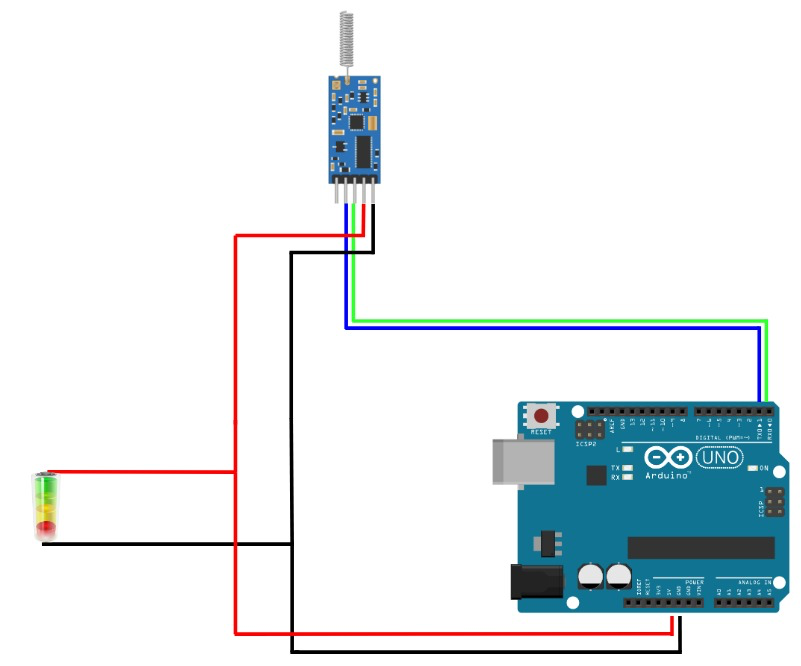
\includegraphics[width=\linewidth]{img/AV/HC12.jpg}
        \caption{HC12 schematic}
    \end{subfigure}
    \begin{subfigure}[b]{.49\linewidth}
        \centering
        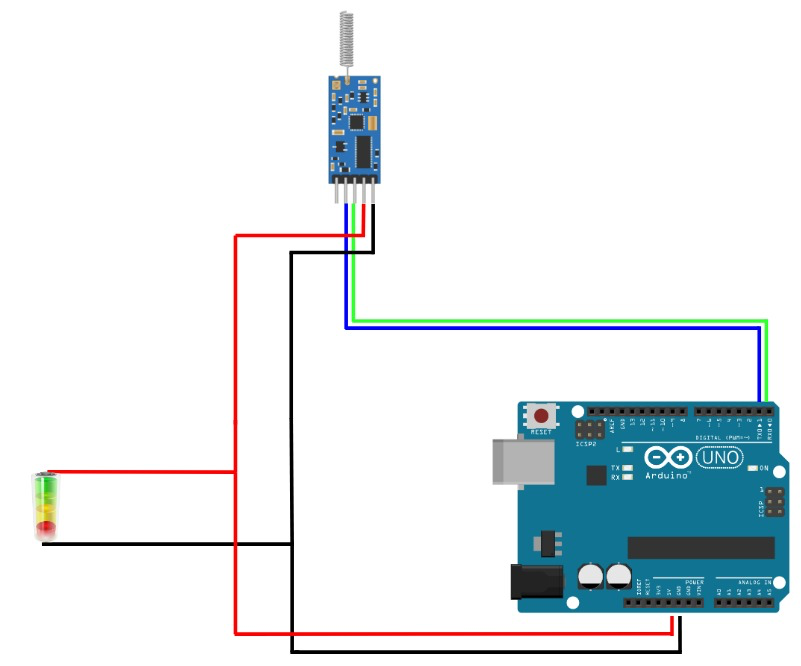
\includegraphics[width=\linewidth]{img/AV/HC12.jpg}
        \caption{HC12 schematic}
    \end{subfigure}
    \caption{HC12 schematics}
\end{figure}

Refer to Table~\ref{tab:Avionics:FMEA}
\begin{table}[htbp]
    \centering
    \caption{Avionics \gls{fmea}}
    \begin{tabularx}{\linewidth}{X l l l X}
        \toprule
        \textbf{Failure Modes} & \textbf{Likelihood} & \textbf{Impact} & \textbf{Risk w/ Mitigation} & \textbf{Mitigation approach} \\
        \midrule
        E-match system failure & 1     & 4     & 1     & Risk is minimized by using ematches in quadruply redundant system. \\\\
        Either parachute deploys prematurely in flight & 1     & 3     & 1     & Risk is minimized by using commercially available altimeters and ematches in quadruply redundant system. \\\\
        Either parachute deploys prematurely on launch pad & 1     & 2     & 1     & A mechanical arming switch that interupts the systems access to power  \\\\
        UAV Deployment system, altimeter brownout & 2     & 4     & 1     & Risk is minimized by extensive redundancy and the Stratologger's 2 second brownout protection. \\\\
        Communications failure & 3     & 3     & 2     & Exstensive testing and use of commericial radios with specifications that far exceed the required range \\\\
        Insufficient Range & 1     & 4     & 1     & Check manufacturer's specfications with range testing under flight conditions (inside rocket or outside) \\\\
        Sensor failure & 3     & 1     & 1     & High quality sensor whose configuration has been validated by prior testing \\ \\
        Short Circuit & 1     & 4     & 1     & Exahustive testing of avionics systems multiple times before final use in rocket \\\\
        Battery Failure & 1     & 4     & 1     & Use voltimeter with batteries and additional testing of avionics systems before final use; Preliminary power consumption calculations \\\\
        \bottomrule
    \end{tabularx}%
    \label{tab:Avionics:FMEA}%
  \end{table}%

  Refer to Table~\ref{tab:Avionics:FMEA}
\begin{table}[htbp]
    \centering
    \caption{Avionics \gls{fmea}}
    \begin{tabularx}{\linewidth}{X l l l X}
        \toprule
        \textbf{Failure Modes} & \textbf{Likelihood} & \textbf{Impact} & \textbf{Risk w/ Mitigation} & \textbf{Mitigation approach} \\
        \midrule
        Battery Damage due to Impact in deployment or communcations system & 2     & 4     & 2     & Make sure both parachutes deploy properly so that impact is not great \\\\
        Disconnection of soldering connections, caused by in-air and launch vibrations & 3     & 4     & 2     & Use tinning when soldering, and possibly choosing solder with silver \\\\
        Wire Disconnection of Deployment System or Communications system, caused by launch vibrations & 1     & 4     & 1     & Make sure soldering connections are solid by taking the precautions above \\\\
        Circuit board splitting, caused by in-air and launch vibrations & 2     & 3     & 2     & Choose circuit board extremely carefully; Exhaustive testing of electronics systems under flight conditions \\
        \bottomrule
    \end{tabularx}%
    \label{tab:Avionics:FMEA 2}%
  \end{table}%
  



\chapter{Flight Dynamics}
The primary responsibility of the Flight Dynamics team is to simulate the performance of both the launch vehicle and the payload, to inform other subteams of constraints that must be satisfied to achieve safe flight, and to make design decisions on all structures and control systems that directly influence the flight of the launch vehicle-payload system.

\section{Simulation Methods}
In order to ensure that predictions of flight performance, as well as insights into possible design improvements, are robust and well-informed, the team is using two different calculation methods to study the flight profile. The team is principally using OpenRocket for simulating the flight of the launch vehicle and predicting critical mission characteristics such as apogee, time to apogee, and total flight time, among many others. OpenRocket is a powerful, open-source rocket flight simulation tool. As it is the most robust and informative, cost-free flight simulation tool available, the team is using it as the primary consultant on aerodynamic design considerations and predicting if the launch vehicle satisfies mission requirements. In addition to predicting flight trajectories, from launch to landing, for various possible initial conditions, OpenRocket also provides baseline estimates for the launch vehicles's mechanical and aerodynamic properties, including pre- and post-burnout masses, drag and lift coefficients, CP and CG locations, stability coefficient, and many others. 
\\*
\newline
As another feature of its versatility, OpenRocket offers multiple customization options for running its trajectory simulations, such as various Earth models and time step size for the numerical integration. To confirm that the simulated trajectories are reliable, the team used two different Earth models, each with a different time step size. The simulation conditions the team used are summarized in the table below.
\FloatBarrier
\begin{table}[H]
\centering
 \caption{OpenRocket simulation conditions}
 \label{tab:FlightDynamics:SimulationConditions}
\begin{tabularx}{.5\linewidth}{llX}
\toprule
 \textbf{Condition} &  \textbf{Time step size [s]} \\
\midrule
   Spherical Approximation &    0.05 \\
    WGS84 &     0.01 \\
\bottomrule
\end{tabularx}
\end{table}
WGS84 (World Geodetic System 1984) is an ellipsoidal model of Earth, and is more accurate than the spherical approximation. Combined with a smaller step size, the trajectory simulation under the WGS84 model is expected to be more accurate than the simulation under the spherical Earth model.

\section{Flight Profile}
The flight profile for this mission features a relatively simple sequence of events.
Nominally at apogee of 4,450ft (and within 2 seconds after apogee), an ejection charge
in the tube coupler will separate the upper and lower body tubes and deploy the drogue parachute. This will be the only explosive separation event of
the entire flight. The main parachute will then deploy at 800ft (this is above the minimum
parachute deployment altitude of 500ft). This was determined to be the optimal altitude because it is high enough to reduce terminal velocity (and thus satisfy the landing kinetic energy requirement), while also being low enough to ensure an acceptable drift distance. 
\\*
\newline
Within two seconds of main parachute
deployment, the solenoid system in the fairing will trigger after the necessary RSO
permission is acquired. Since the nose cone is sized to fit loosely into the fairing, releasing the solenoids will allow the nose cone to slide freely from the fairing, from which point it will descend the remainder of the altitude independently. The nose cone will also be equipped with its own parachute, which will be secured with a Jolly Logic chute release. This device will be programmed to release the parachute at a pre-determined altitude, which is currently planned to be 400ft. Once the parachute is released, it will be unfurled by the low pressure region in the nose cone's wake. 
\\*
\newline
Immediately upon release of the nose cone by the solenoid system, the drone will passively slide out from the fairing under the influence of gravity, guided by a rail system to which it will be attached until deployment. Unlike the nose cone, the drone will be attached to the fairing by a lowering mechanism. This lowering mechanism will allow the drone to hang exposed to the free stream, enabling it to conduct the necessary observations to pass the on-board safety checklist, while using minimal thruster power. If the drone determines itself to satisfy the pre-specified conditions for safe flight, it will cut itself from the mechanism, and proceed with the mission.
\\*
\section{Simulation Results}
The flight profile was simulated in OpenRocket using a model of the rocket with numerous
design specifications (e.g. fin and body tube dimensions, material, and motor type), various initial
conditions, and even the exact coordinates of the launch site. Per competition requirements, the wind speed was varied between 0-mph, 5-mph, 10-mph, 15-mph, and 20-mph, and held constant during each simulation. To account for the launch rail being canted away from the crowd on launch day to offset wind conditions, the launch angle was also varied for certain values between 5 and 10 degrees. 
\\*
\newline
Current projections show the rocket to satisfy all requirements of flight performance, thus validating the current flight profile. If
necessary, the flight profile can be adjusted to better accommodate these requirements;
for example, the altitude of main parachute deployment can be lowered to ensure that the
drift distance remains within the recovery area.
\subsection{Vehicle Stability}
As mentioned above, OpenRocket simulates mechanical properties of the launch vehicle in addition to its trajectory, based on the constructed model. The model constructed in OpenRocket includes all of the critical components that will be part of the final design; these include: payload, fairing and coupler avionics bays, and drogue and main parachutes. Based on this model, OpenRocket calculated the launch vehicle static stability margin to be 2.4, which satisfies the minimum required static stability margin of 2.0. The OpenRocket model is shown in the figure below.
\begin{figure}[h]
\centering
    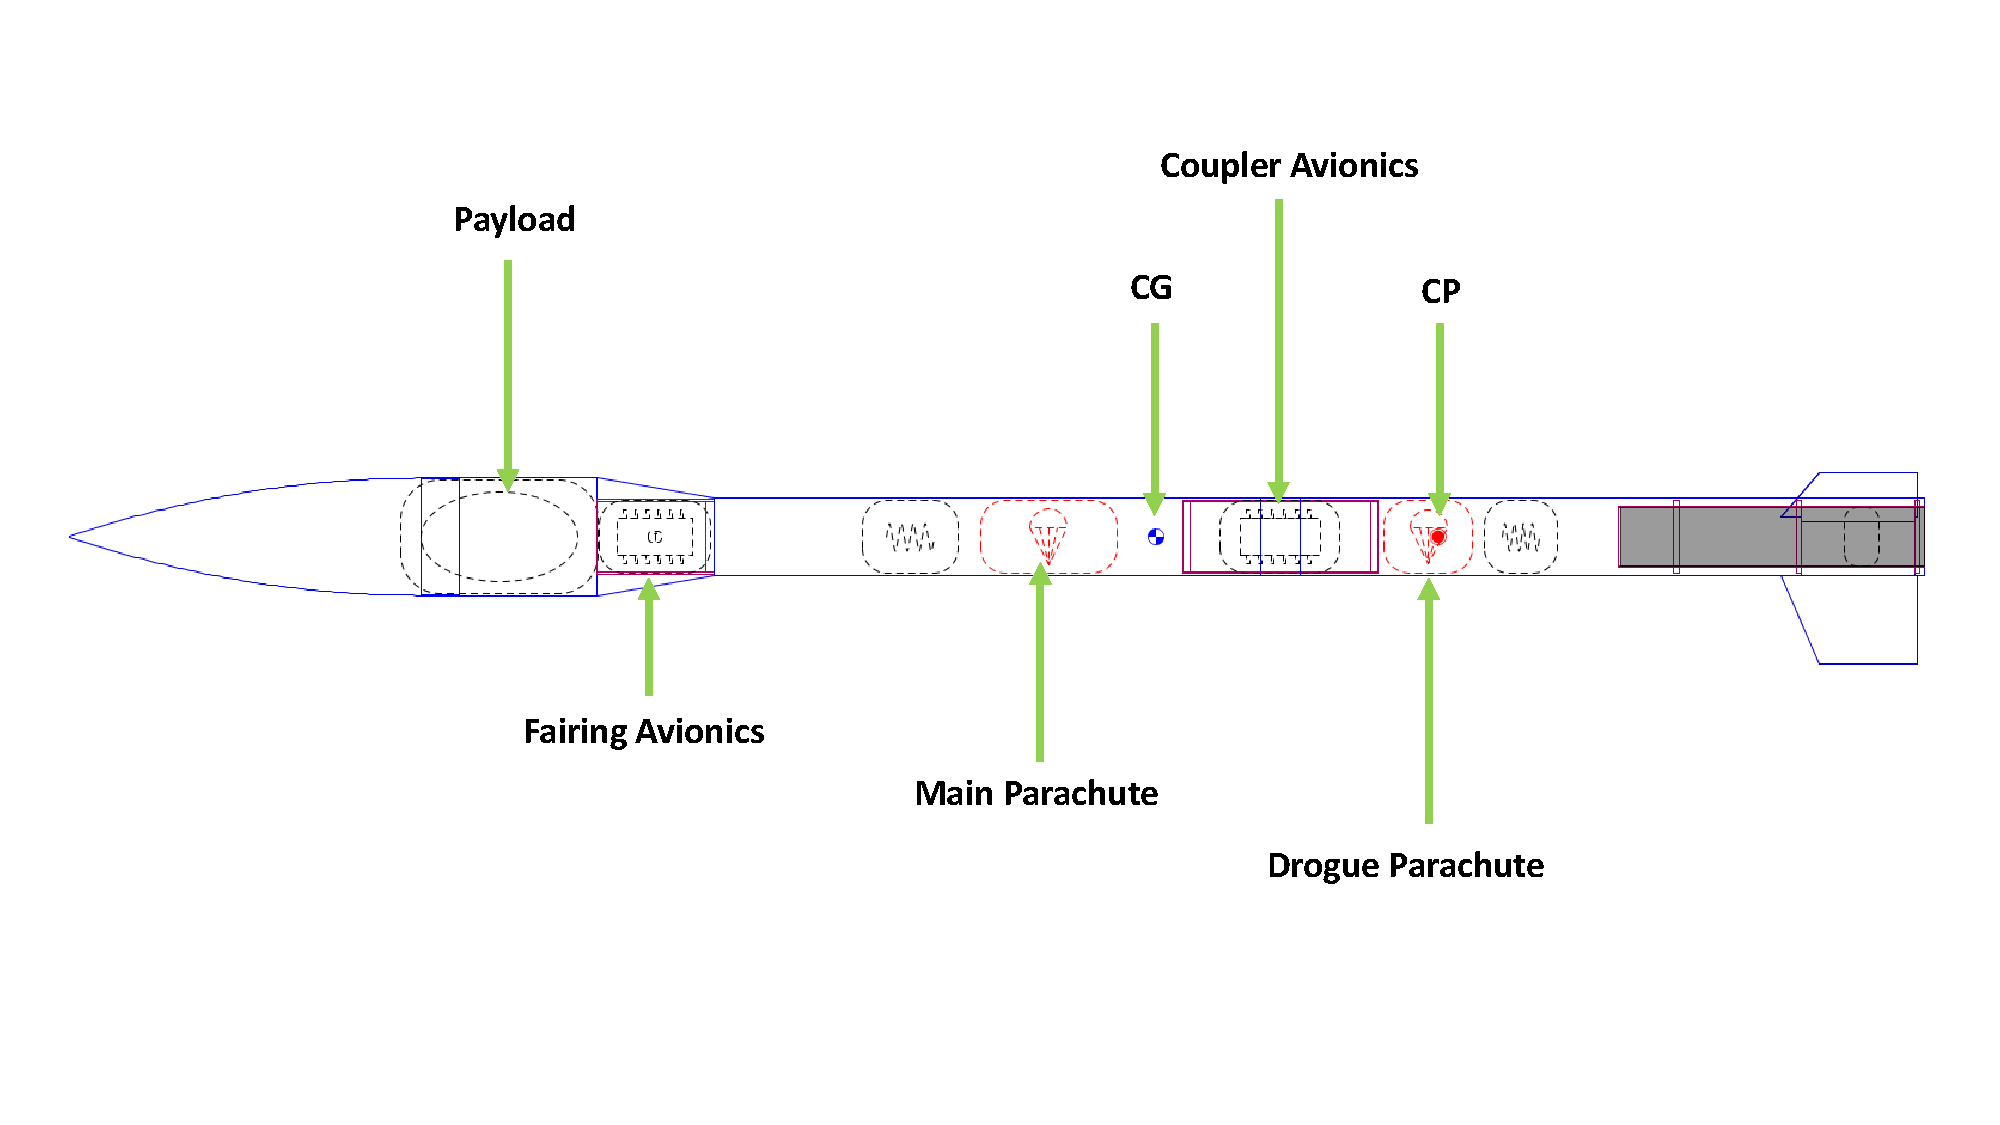
\includegraphics[width = 14cm, height = 7cm]{img/FIDO/openrocket_Model.pdf}
    \caption{OpenRocket model of launch vehicle, with various points of interest highlighted.}
    \label{fig:my_label}
\end{figure}   

\subsection{Kinetic Energy and Descent Time Predictions}
For each combination of launch parameters, the team simulated the trajectory of the launch vehicle under the spherical Earth condition (with time step 0.05s) and customized the simulations to yield data for the speed and altitude of the vehicle as functions of time. This data was used to demonstrate satisfactory flight duration and terminal kinetic energy. Specifically, the terminal specific kinetic energy was calculated using the following equation:
\begin{equation}
        t = \frac{v{_T}^2}{2}
\end{equation}
Where $v{_T}$ is the terminal velocity upon landing. Note that all components of the vehicle (lower body tube, upper body tube, and nose cone) are assumed to land at the same terminal velocity. The table below summarizes the data from these simulations that pertains to descent and landing.

\begin{table}[H]
    \centering
    \caption{Terminal descent characteristics for various launch parameters (spherical Earth condition)}
    \label{tab:FlightDynamics:TerminalDescentCharacteristics}
    \begin{tabularx}{\linewidth}{lllXX}
    \toprule
     \textbf{Angle [deg]} &  \textbf{Wind [mph]} &  \textbf{Descent time [s]} &  \textbf{Term. desc. velocity [m/s]} &  \textbf{Term. spec. kinetic energy [J/kg]} \\
    \midrule
       5.0 &     0 &        72.822 &               -7.4420 &                   27.691682 \\
       5.0 &     5 &        72.338 &               -7.4417 &                   27.689449 \\
       5.0 &    10 &        71.319 &               -7.4424 &                   27.694659 \\
       5.0 &    15 &        71.111 &               -7.4421 &                   27.692426 \\
       5.0 &    20 &        70.144 &               -7.4424 &                   27.694659 \\
       7.5 &     0 &        71.904 &               -7.4418 &                   27.690194 \\
       7.5 &     5 &        71.190 &               -7.4429 &                   27.698380 \\
       7.5 &    10 &        70.578 &               -7.4418 &                   27.690194 \\
       7.5 &    15 &        70.118 &               -7.4425 &                   27.695403 \\
       7.5 &    20 &        69.532 &               -7.4416 &                   27.688705 \\
      10.0 &     0 &        72.241 &               -7.4424 &                   27.694659 \\
      10.0 &     5 &        71.485 &               -7.4420 &                   27.691682 \\
      10.0 &    10 &        70.633 &               -7.4417 &                   27.689449 \\
      10.0 &    15 &        68.627 &               -7.4421 &                   27.692426 \\
      10.0 &    20 &        68.321 &               -7.4414 &                   27.687217 \\
    \bottomrule
    \end{tabularx}
\end{table}
The table shows that the descent time of the launch vehicle system in all simulated cases is well below the maximum allowed descent time of 90 seconds. Therefore, the team expects each of the components of the vehicle to descend from apogee within the maximum allowed time.
\\*
\newline
From the terminal specific kinetic energy data, the terminal kinetic energy can be calculated for each individual component by simply multiplying the specific kinetic energy by the mass of the component:
 \begin{equation}
    T{_c} = m{_c}*t    
 \end{equation}
To demonstrate that the impact kinetic energy requirement is satisfied, the team calculated the terminal kinetic energy of each component under the "worst-case scenario", or the simulated scenario with the highest terminal specific kinetic energy.  The results of these calculations are summarized in the table below.

\begin{table}[H]
\centering
\caption{Terminal kinetic energy of each component in worst-case scenario (spherical Earth condition)}
\label{tab:FlightDynamics:TerminalKineticEnergy}
\begin{tabularx}{.5\linewidth}{XlX}
\toprule
  \textbf{Component} & \textbf{Mass [kg]} &  \textbf{Term. kinetic energy [J]} \\
\midrule
Nose cone & 0.626 &             17.339186 \\
Fairing & 1.114 &             30.855996 \\
Upper body & 1.221 &             33.819722 \\
Switch band & 0.771 &             21.355451 \\
Lower body & 3.570 &             98.883217 \\
\bottomrule
\end{tabularx}
\end{table}

As can be seen, the terminal kinetic energy of each component (under the assumption that each component lands at the same terminal velocity) is less than the maximum allowed value of 101.69J (75ftlb). Therefore, according to OpenRocket, even under the most unfavorable launch characteristics, the launch vehicle still satisfies the impact energy requirement.

\subsection{Drift and Apogee Predictions}
The landing point of the launch vehicle is a critical safety concern to all parties and property in the area. To mitigate this risk, the team conducted several trajectory simulations for various wind speeds, launch angles, and simulation conditions. To visualize the drift, the trajectories were plotted on an in-plane graph, where the y-axis is north-south and the x-axis is east-west. The plots for the spherical Earth approximation condition are shown below.
\FloatBarrier
\begin{figure}[h]
    \centering
    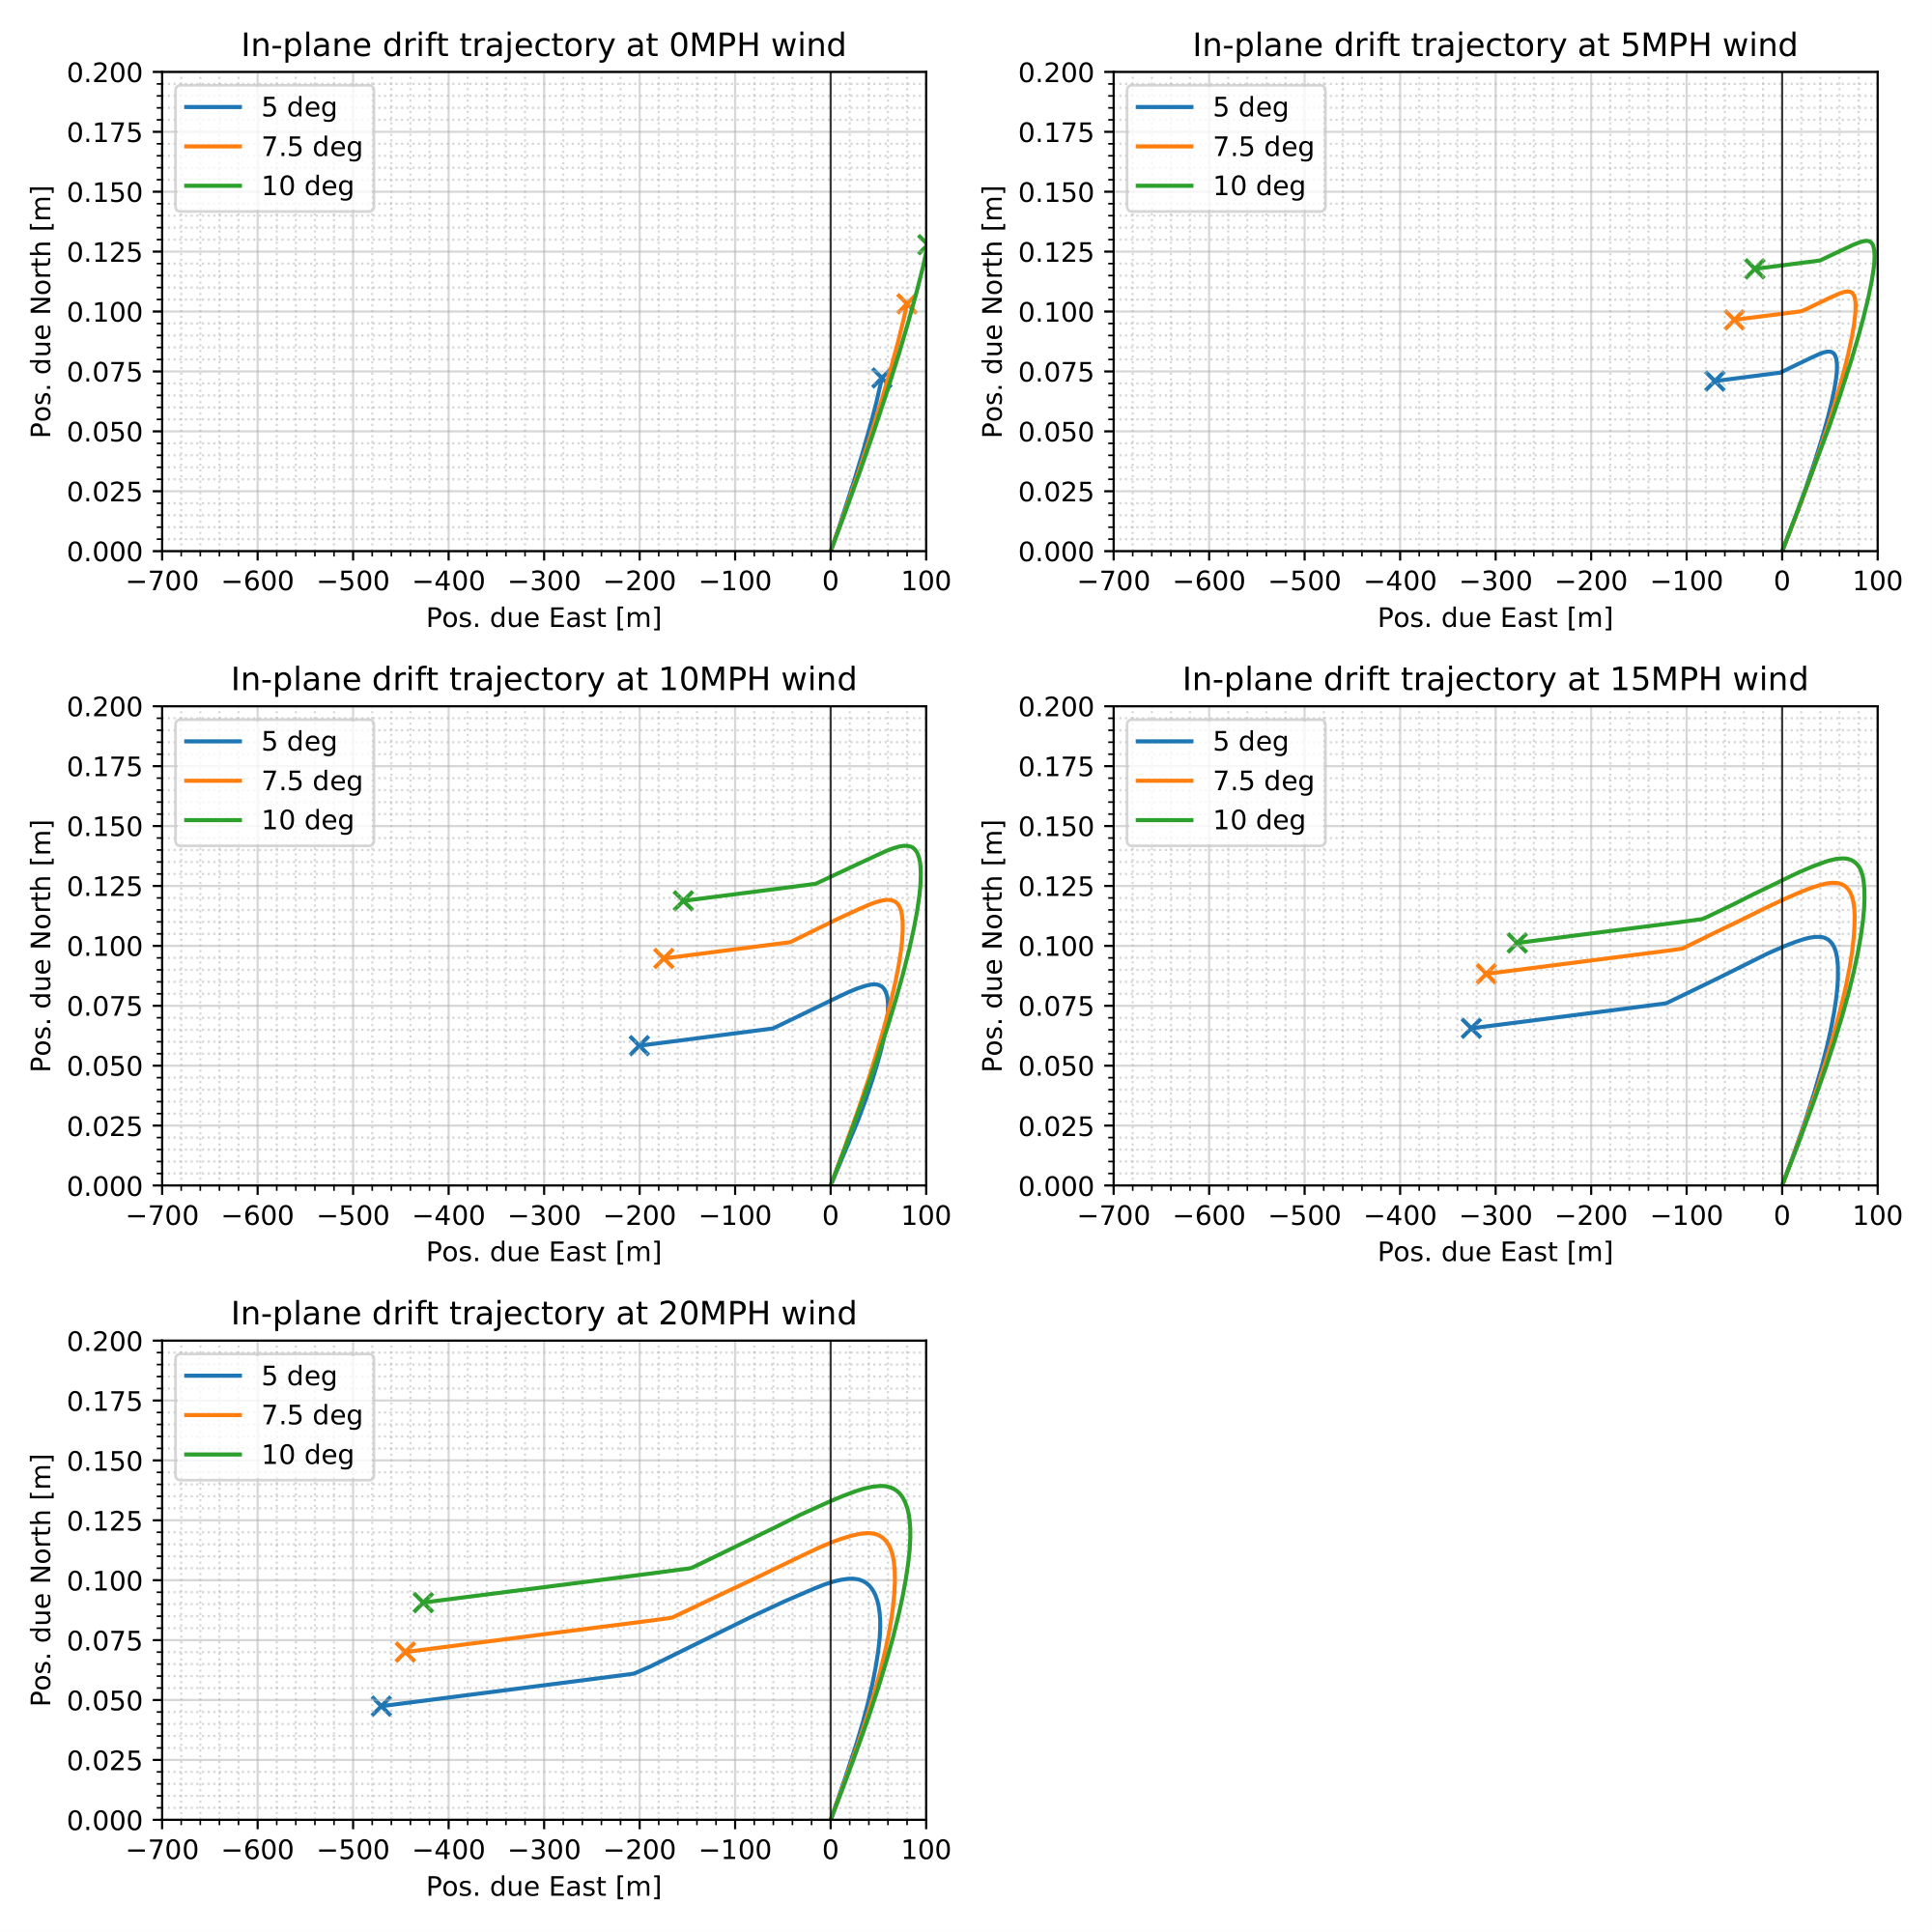
\includegraphics[width = 15cm, height = 11cm]{img/FIDO/InPlaneDrift-1.png}
    \caption{Predicted in-plane drift for various wind speeds and launch angles (all under spherical Earth approximation condition)}
    \label{fig:my_label}
\end{figure}
Note that, given the scaling of the north-south axis, the trajectories in each of these simulated scenarios is almost purely in the east-west direction. The most extreme landing displacement from the launch pad appears to occur in the 20-mph wind, 5 degree launch angle case, where the predicted landing distance from the launch pad is about 500m (about 1,640ft). Thus, even under the most extreme launch scenarios, the team expects the launch vehicle system to land well within the radius of the recovery area.
\\*
\newline
For the sake of comparison, the team conducted the exact same simulations for the WGS84 condition. The resulting plots are shown below.
\FloatBarrier
\begin{figure}[h]
    \centering
    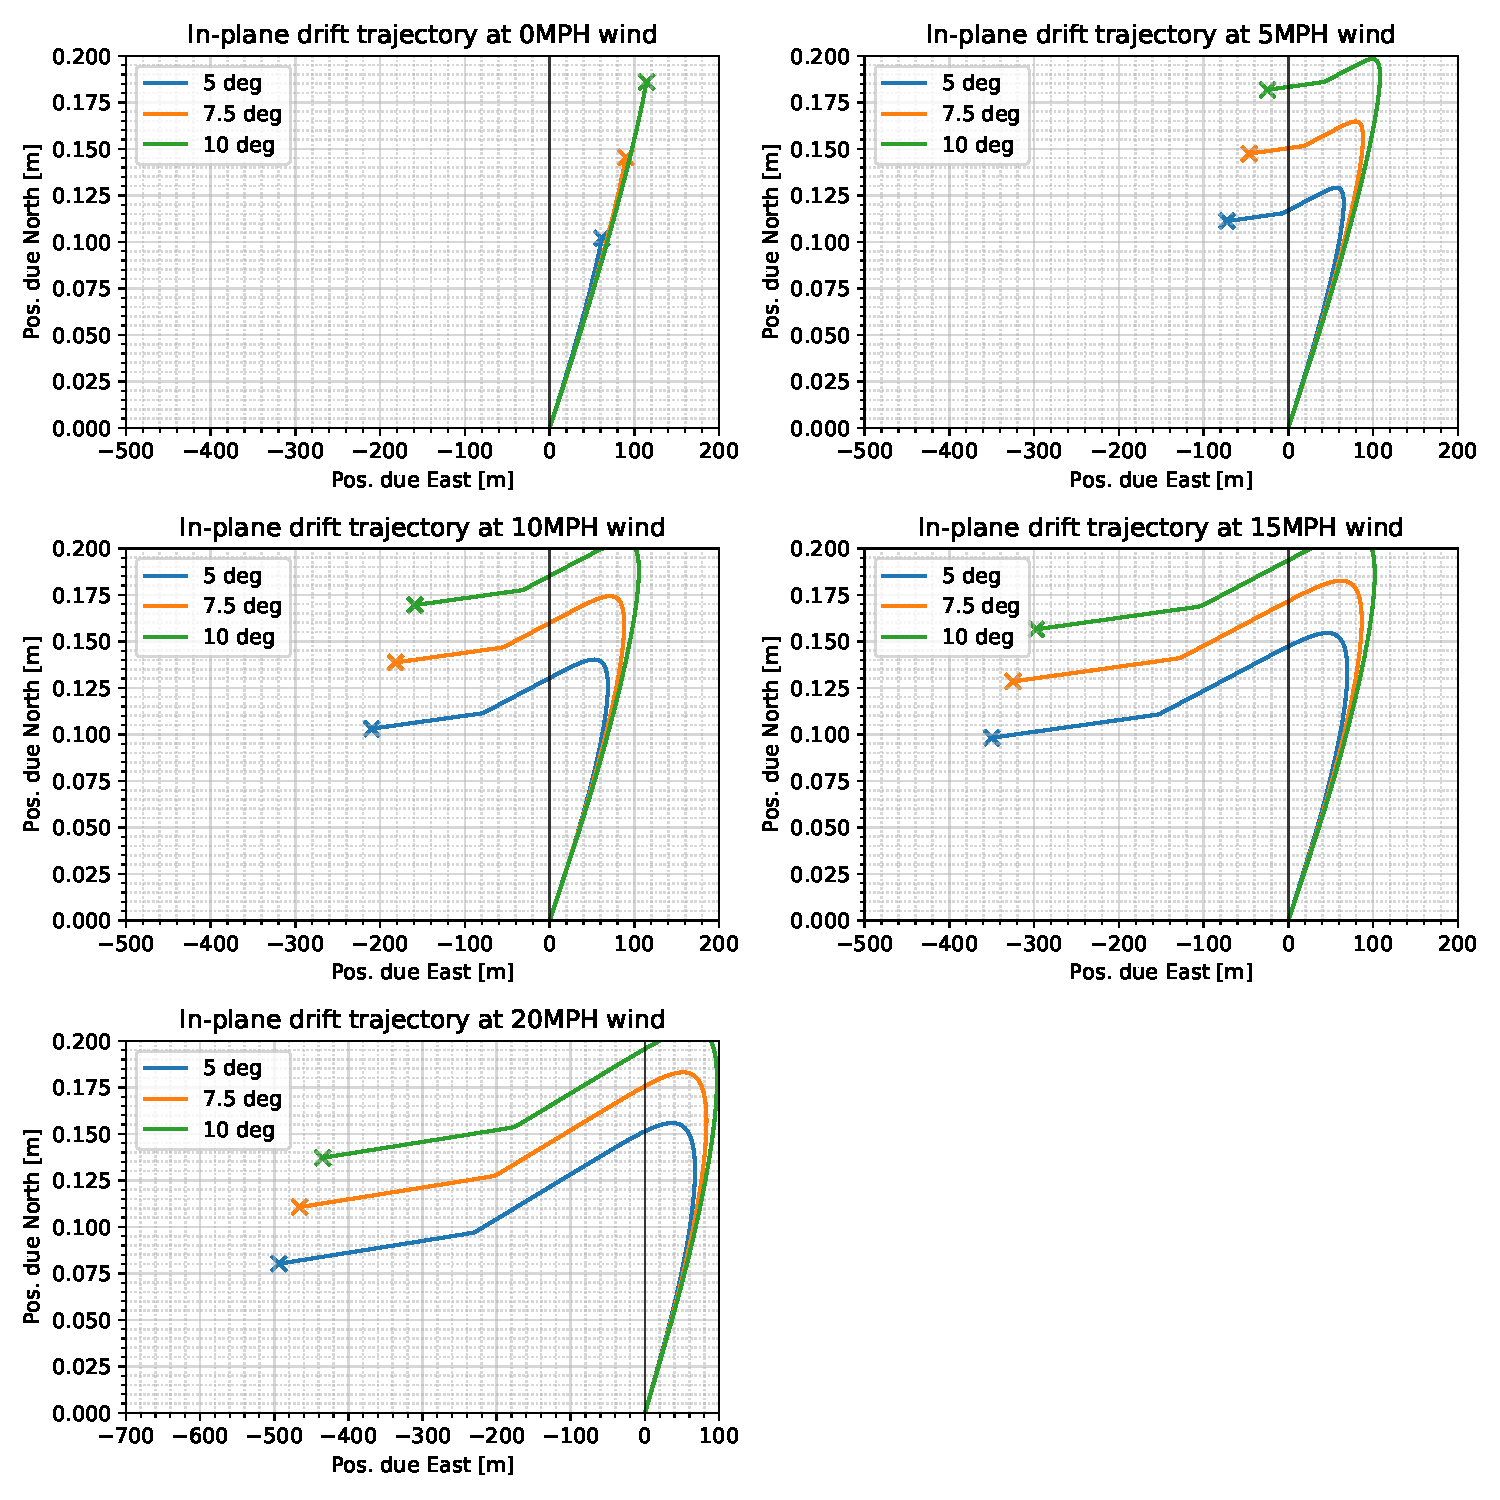
\includegraphics[width = 15cm, height = 11cm]{img/FIDO/InPlaneDriftWGS.pdf}
    \caption{Predicted in-plane drift for various wind speeds and launch angles (all under WGS84 condition)}
    \label{fig:my_label}
\end{figure}
\FloatBarrier
While the WGS84 and spherical Earth approximation conditions predict slightly different drift trajectories, neither of them predict a maximum possible landing distance from the launch pad over 500m (about 1,640ft), thus both simulation conditions provide compelling evidence that the launch vehicle system will land within the recovery area radius.
\\*
\newline
To determine the target apogee, the team also plotted the altitude data as a function of time from the same simulated trajectories.
\begin{figure}[h]
    \centering
    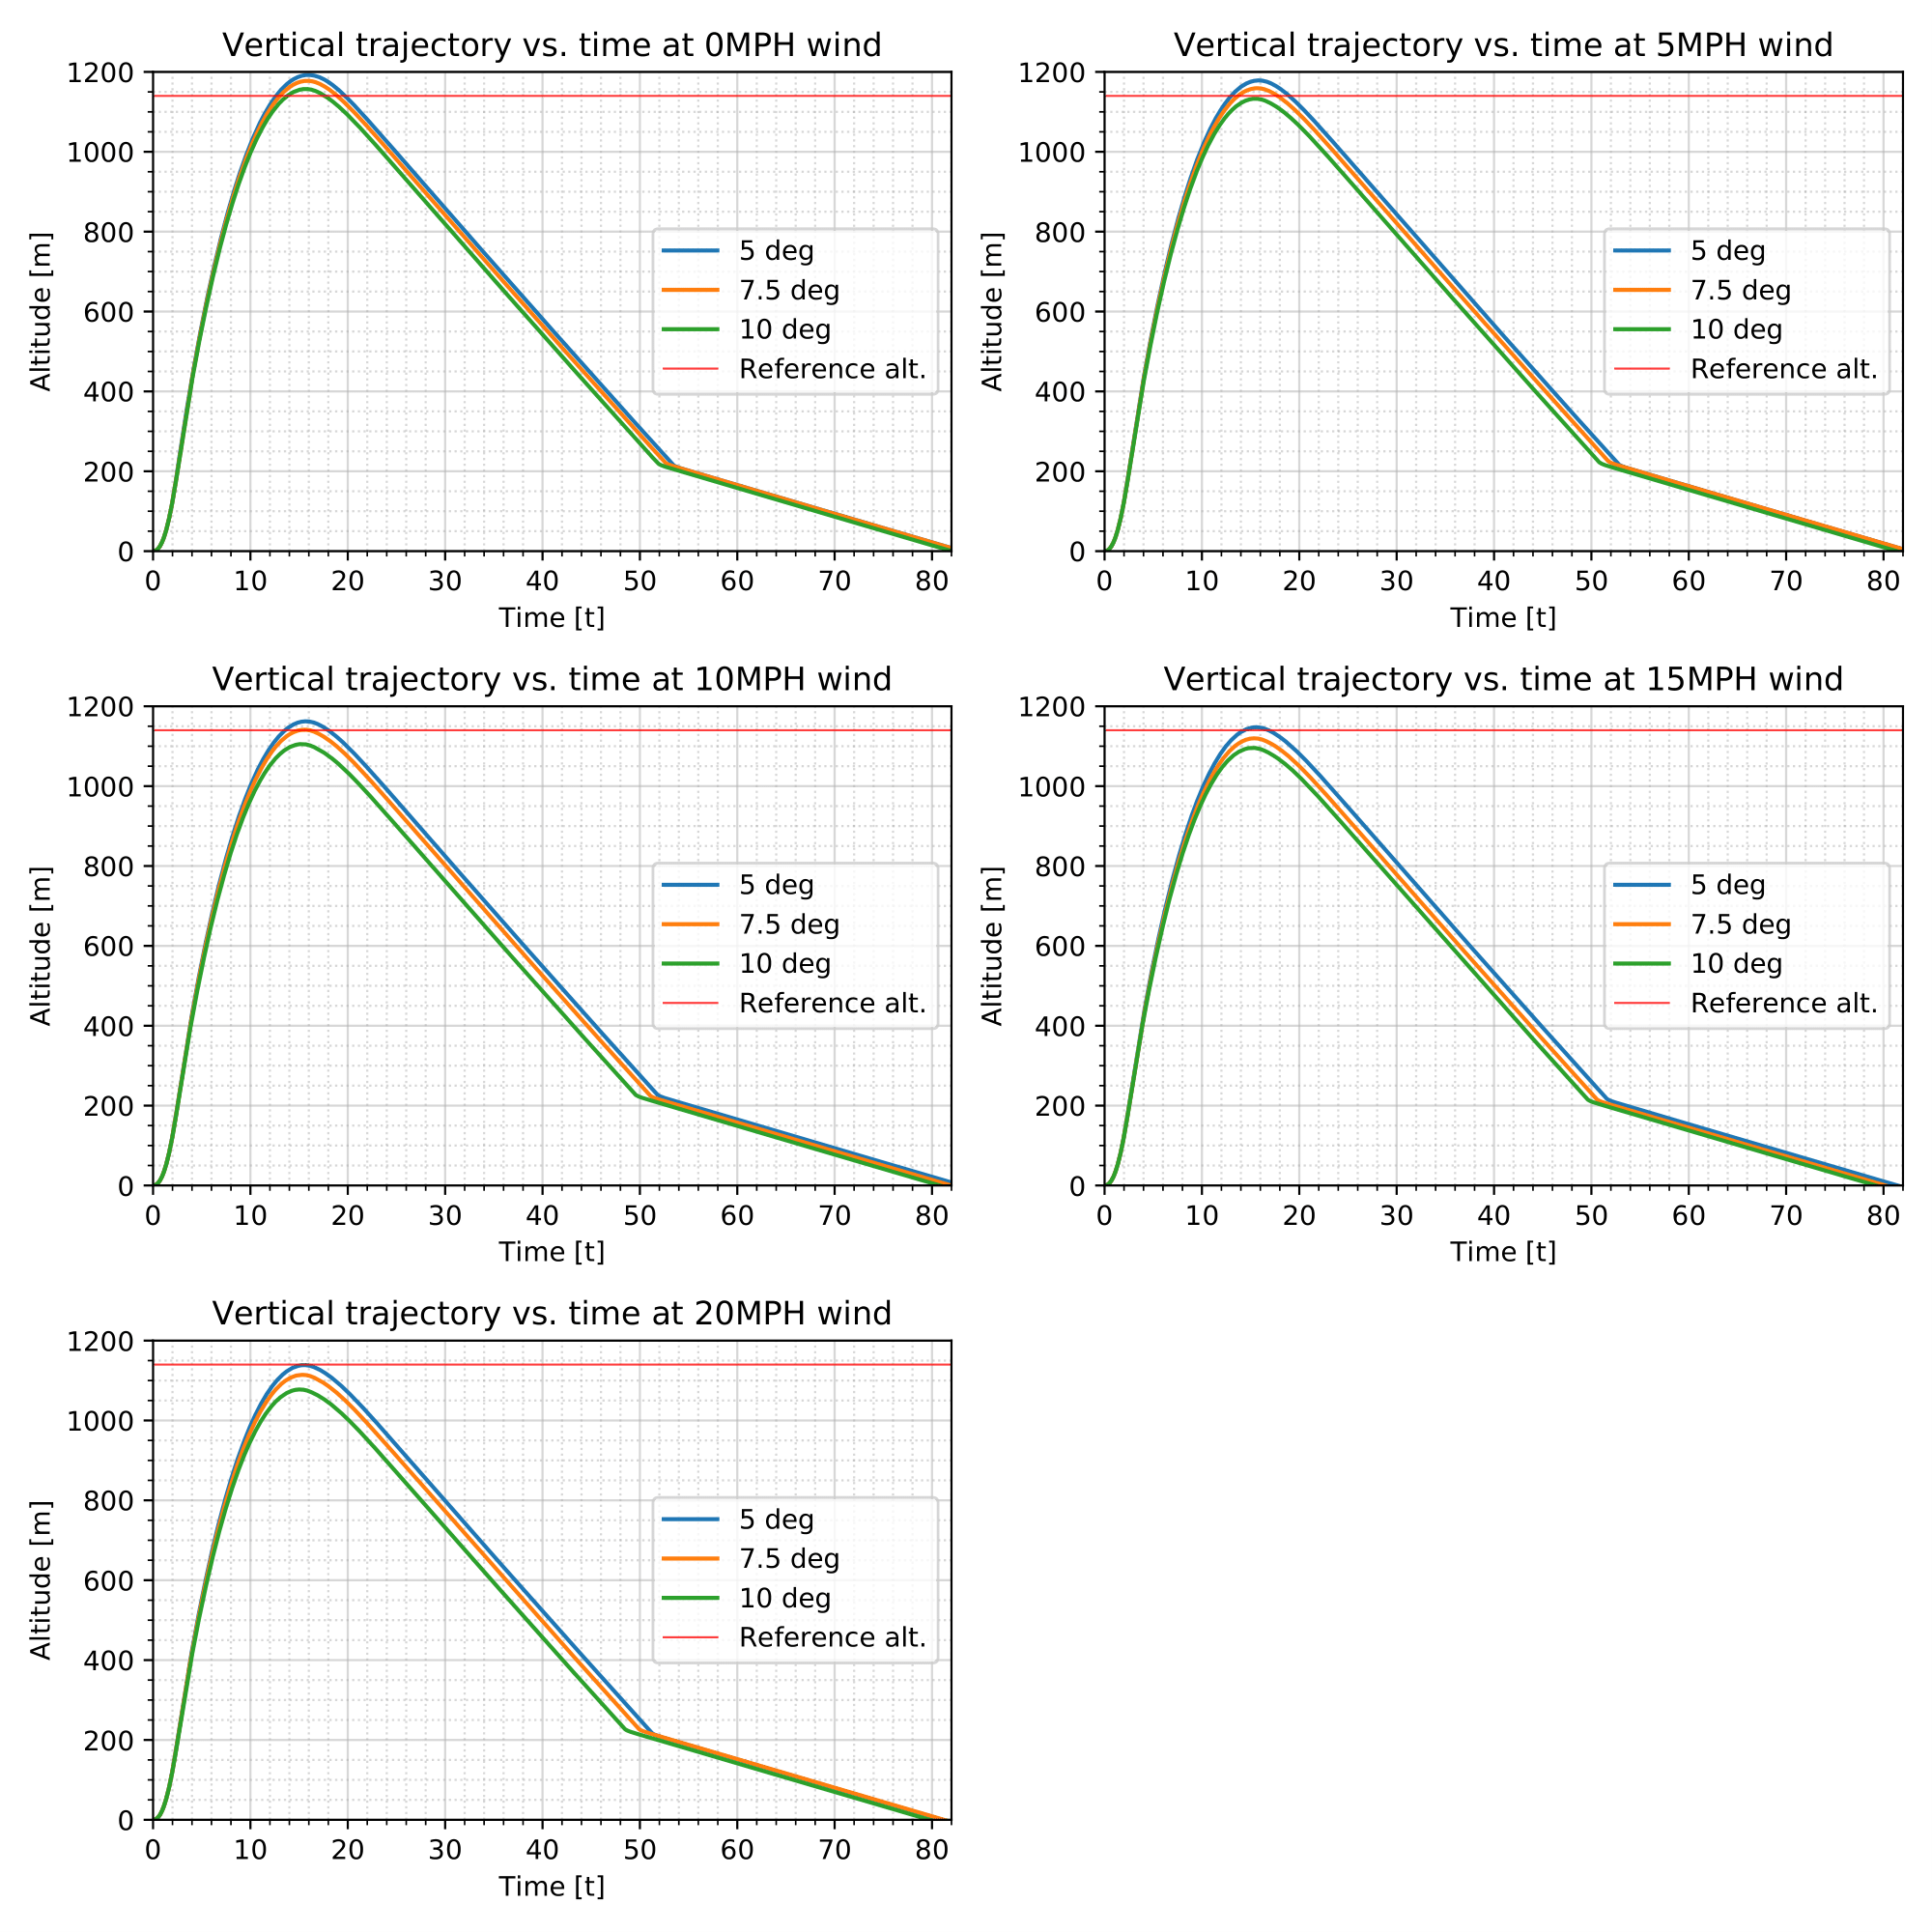
\includegraphics[width = 15cm, height = 11cm]{img/FIDO/VerticalTrajectory-1.png}
    \caption{Simulated altitude as a function of time for various wind conditions and launch angles (spherical Earth approximation condition)}
    \label{fig:my_label}
\end{figure}
\begin{figure}[h]
    \centering
    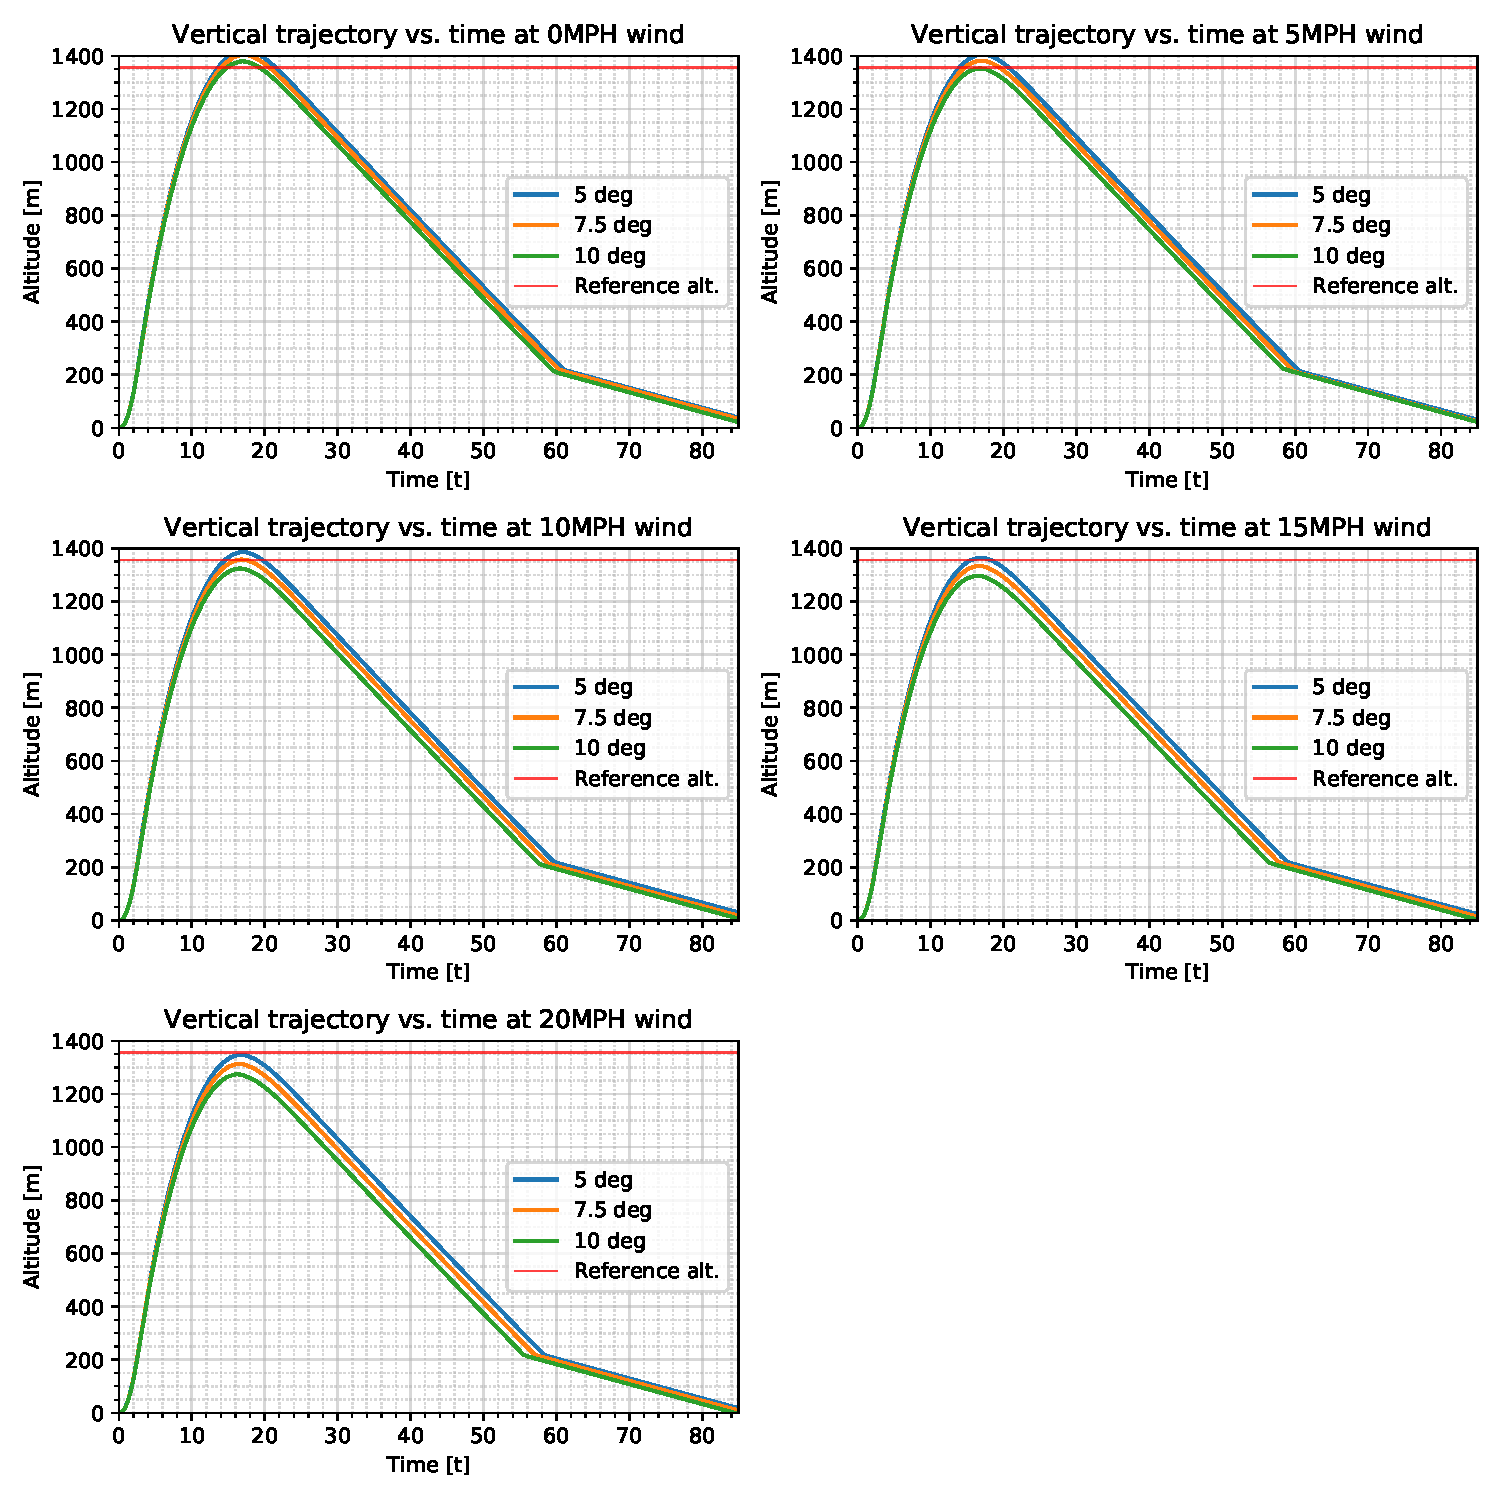
\includegraphics[width = 15cm, height = 11cm]{img/FIDO/VerticalTrajectoryWGS.pdf}
    \caption{Simulated altitude as a function of time for various wind conditions and launch angles (WGS84 condition)}
    \label{fig:my_label}
\end{figure}
\FloatBarrier
As can be seen in the plots above, the spherical Earth approximation and WGS84 conditions predictions of apogee differ significantly, in some cases by over 200m (over 656ft). However, as discussed previously, the WGS84 simulation condition is expected to be more accurate because it is a more accurate Earth model with a smaller time step size. As a result, the team primarily based its target altitude decision on the WGS84 simulation condition. The team has determined its official target altitude to be 4,450ft.
\begin{table}[H]
\centering
\caption{Official target altitude}
\label{tab:FlightDynamics:TargetAltitude}
\begin{tabularx}{.5\linewidth}{XlX}
\toprule
  \textbf{Target altitude [ft]}\\
\midrule
4,450 \\
\bottomrule
\end{tabularx}
\end{table}

\section{Simulation Discrepancies}
As the team ran simulations for the two different conditions (WGS84, spherical Earth approximation), the projected trajectories were typically found to have relatively minor discrepancies. To quantify the difference in results of the two simulation conditions, the time series data of altitude for each set of launch characteristics (launch angle and wind speed) from the spherical Earth approximation condition was subtracted from the WGS84 condition. This was done to calculate the root-mean-square (RMS) error of the difference between the two simulation conditions. The result of these calculations are shown in the table below.
\begin{table}[H]
\centering
\caption{Normalized root-mean-square error between the two simulation conditions for all launch parameters}
\label{tab:FlightDynamics:AverageError}
\begin{tabularx}{.5\linewidth}{llX}
\toprule
 \textbf{Angle [deg]} &  \textbf{Wind [mph]} &  \textbf{Error norm [m]} \\
\midrule
   5.0 &     0 &    0.558017 \\
   5.0 &     5 &    0.821123 \\
   5.0 &    10 &    0.906802 \\
   5.0 &    15 &    0.529063 \\
   5.0 &    20 &    0.567203 \\
   7.5 &     0 &    1.070750 \\
   7.5 &     5 &    0.152635 \\
   7.5 &    10 &    0.350443 \\
   7.5 &    15 &    0.332065 \\
   7.5 &    20 &    0.547357 \\
  10.0 &     0 &    1.646402 \\
  10.0 &     5 &    0.161091 \\
  10.0 &    10 &    1.463531 \\
  10.0 &    15 &    0.613284 \\
\bottomrule
\end{tabularx}
\end{table}
As can be seen, the average difference in predicted altitude over time between the two simulation conditions across all sets of simulated launch parameters (launch angle and wind speed) never exceeded 2m. Thus, the team is confident that the simulated trajectories provided by OpenRocket are sufficiently reliable to guide further design considerations and developments of the launch vehicle and mission profile. 


\part{Structures}

\chapter{Launch Vehicle Breakdown}

\section{Launch Vehicle Overview}
The launch vehicle will be 7 feet and 11 inches tall with a diameter transitioning from 4 to 6 inches. It will consist of three distinct sections: booster tube, body tube and interstage, and nosecone. The total mass of the launch vehicle will be 24.7 pounds. The chosen motor is the Aerotech K780R-P which will take the launch vehicle to an apogee of 4,450 feet above ground level. At apogee, a 20 inch drogue parachute will be deployed and the launch vehicle will fall under this parachute until 800 feet. . At 800 feet above the ground, a 70-inch main parachute will deploy until the launch vehicle lands safely. The nose cone will separate at 400 feet and descend with its own parachute, exposing the payload bay and allowing the UAV to deploy. Further details are explained in other portions of this preliminary design review.

\FloatBarrier
\begin{figure}[h]
    \centering
    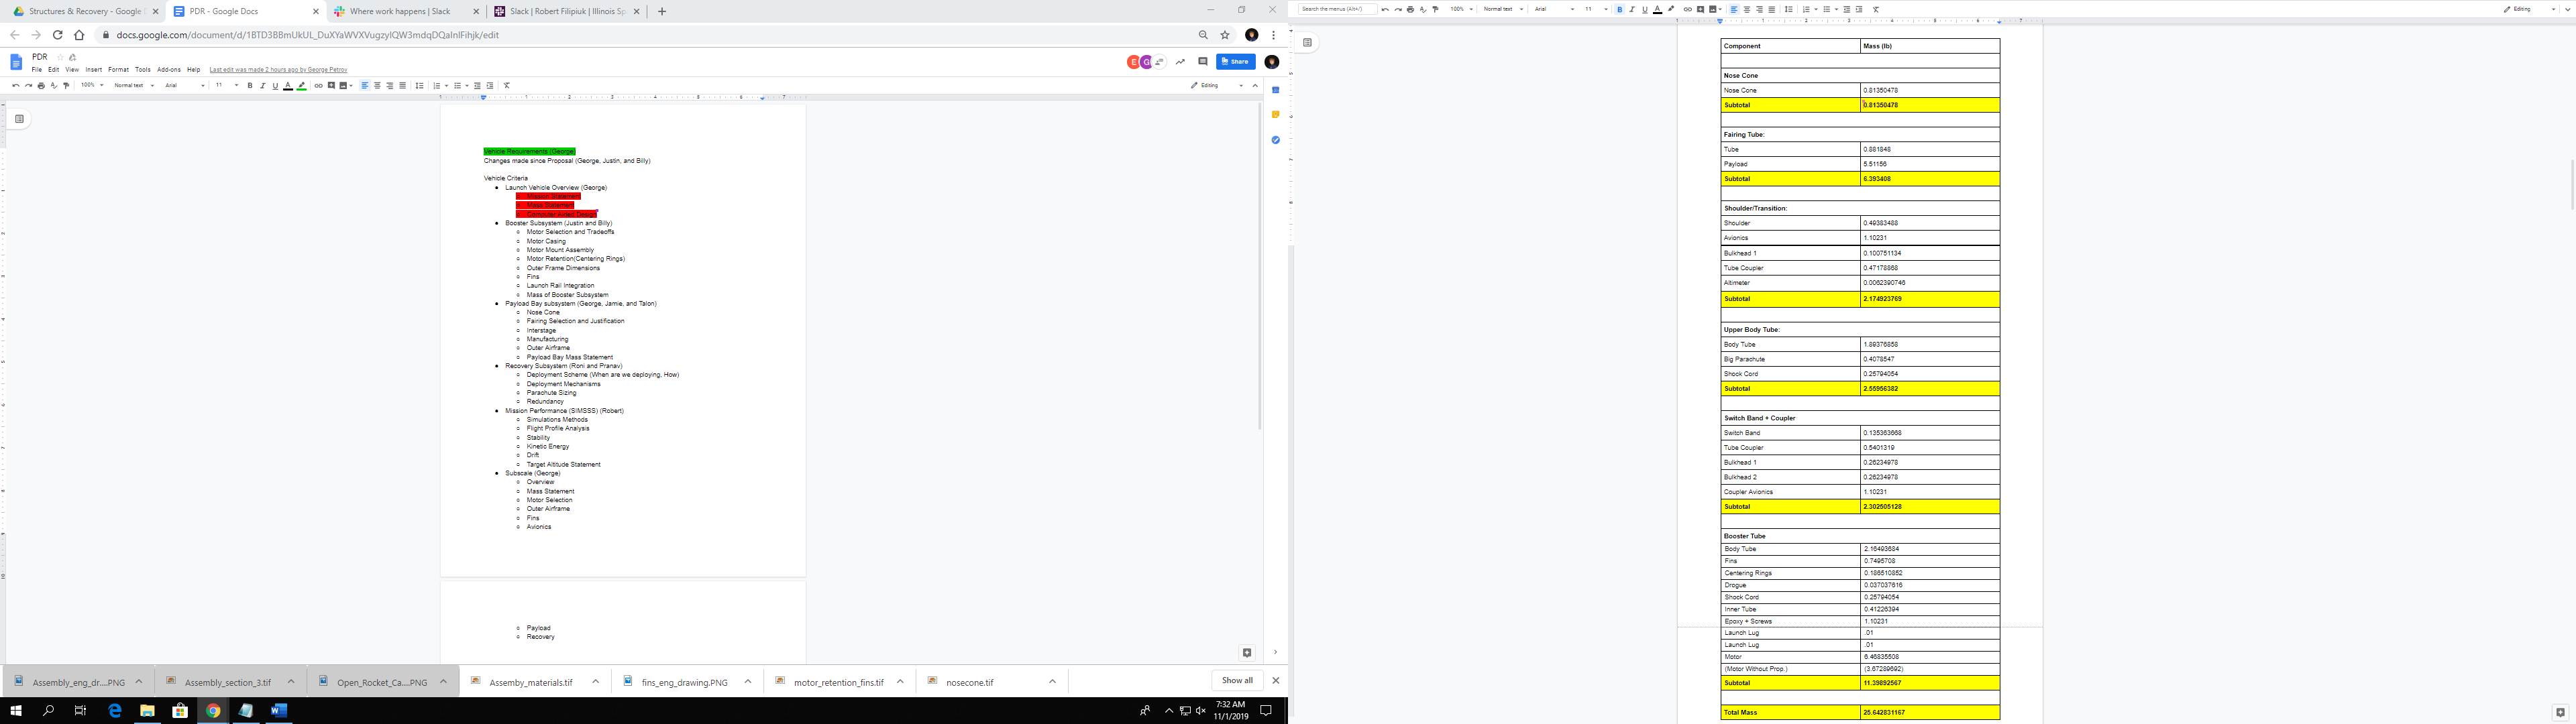
\includegraphics[width = 15cm, height = 20cm]{Masses.png}
    \caption{Predicted in-plane drift for various wind speeds and launch angles (all under spherical Earth approximation condition)}
    \label{fig:my_label}
\end{figure}

    \subsection{Mission Statement}
The rocket will ascend to a predefined altitude and return to the ground under parachutes. During descent, a drone will be deployed that is capable of detaching and flying to a target area to retrieve samples. The entirety of the mission will be conducted in accordance with all rules set forth by NASA in the 2020 NASA Student Launch Handbook.
   
    

\section{Booster Subsystem}
The booster subsystem is the lowest portion of the launch vehicle. It is primarily responsible for producing and properly containing the thrust of the rocket. The fins provide stability for the vehicle, ensuring a nominal trajectory. This subsystem also includes structural components that are necessary for safety and aerodynamics.

The main components of the booster subsystem are the motor, motor casing, motor mount, centering rings, outer airframe, and fins. Thrust is produced by the motor, while the motor casing, motor mounts, and centering rings are used to ensure the motor will maintain the correct orientation. The centering rings are mounted to the outer airframe and are arranged in such a way to direct the thrust vector through the vehicle’s center of mass.

The fins are an aerodynamic structure which collectively ensure stability and passive control for the launch vehicle. The overall subsystem is constructed to make sure that the rocket exits the launch rail with the desired velocity and stability and reaches the intended final altitude. A CAD model of the booster section is shown in [FIGURE HERE].

    \subsection{Motor Selection}
For the 2019-2020 Student launch competition, the team has chosen to use the AeroTech K780R-P motor. This motor satisfies all competition requirements since it keeps the target apogee within 3,500 feet and 5,500 feet above ground level, expels ammonium perchlorate composite propellant (APCP) during launch, has an impulse below the 5,120 Newton-Second limit, accelerates the launch vehicle beyond 52 feet per second upon exiting the rail, does not expel titanium sponges, is not a hybrid motor, is not clustered, and will not propel the launch vehicle above Mach 1 based on simulations. The motor is also able to be ignited using a 12-volt firing system and does not utilize any forward firing motors. According to updated OpenRocket simulations and the characteristics of the selected motor, the vehicle’s thrust-to-weight ratio is 8.5:1. Thrust-to-weight ratios greater than 5 are typically considered safe for high-powered rockets.

Performance specifications [TABLE BELOW] and a thrust curve diagram [FIGURE BELOW] for the K780R-P motor were found at thrustcurve.org. The motor reaches a maximum thrust of 216.9 pounds-force in about 1.15 seconds. The motor provides an average thrust of 175.4 pounds-force with a total burn time of 3.0 seconds.

In summary, the AeroTech K780R-P motor was chosen because it satisfies all necessary requirements stated within the guidelines provided for the Student Launch Competition. Other motors such as the Aerotech K1000T-P and Animal Motor Works K605RR were considered in the final decision, but it was determined that Aerotech was the favorable brand due to Illinois Space Society’s previous success with them, and the K1000T-P proved to provide too much impulse and caused the apogee to exceed competition guidelines with the final design of the rocket. Additionally, when compared to the K1000T-P, the K780R-P has lower acceleration over a slightly longer burn time, meaning structural loads on the rocket and payload are reduced.

    \subsection{Motor Casing}
The Aerotech 75/2560 motor casing will be used to house the K780R-P motor. It is the casing associated with this motor. It is made of aluminum, allowing it to withstand the high temperatures and forces created by the motor during launch. In addition, the top of the casing will serve as the lower attachment point for the drogue parachute. The length of the case is 15.577 inches with a diameter of 3.0 inches.


    \subsection{Motor Mount Assembly}
The motor mount assembly will consist of the motor mount tube, centering rings, and fins. The purpose of the motor mount is to keep the motor and motor casing in a stable position during flight. The motor mount tube will be constructed from a 15-inch length of Blue Tube with an outer diameter large enough to accomodate the motor casing. This tube, held in place by three fiberglass centering rings, will house the motor and motor casing.

Fiberglass was chosen for the centering rings as it is a strong material that will reduce the movement of the motor as much as possible without threat of deformation. These centering rings will have a thickness of 0.125 inches, and each will be epoxied onto the outside of the motor mount tube. The motor mount assembly also provides a rigid mount point for the fins. The three fiberglass fins will have fin tabs with a depth of 0.3 inches and a length of 5.2 inches beginning 1.2 inches from the bottom of the fin. This will allow them to be epoxied between the two lower centering ring prior to the insertion of the entire assembly into the lower airframe. An engineering drawing of the fin design can be seen in [FIGURE HERE]


    \subsection{Motor Retention}
A 2.95-inch Aero Pack motor retainer will be utilized. It is an aluminum part designed to keep the motor securely within the rocket during flight, as well as allow for quick and simple loading and unloading of the motor. The retainer will be screwed into the lower centering ring of the booster tube. Locknuts will be used on the opposite side of the screws holding in the retainer, ensuring that the connection will not be compromised in the event of high vibrations during flight. Though the screws are meant to allow reusability, the retainer will additionally be epoxied to the centering ring to provide added assurance that it will not come apart under any conditions. This mounting mechanism is threaded and has a matching cap that can be screwed on over the motor, thereby retaining it.

    \subsection{Outer Frame Dimensions}
In selecting a material for the outer airframe, the team considered three options: Blue Tube, fiberglass, and carbon fiber. Unanimously, the team voted on Blue Tube for the body tube and booster tube sections because of its low cost and its lower density, contributing less mass to the vehicle compared to fiberglass and carbon fiber. This low-cost, low-density justification is solely for these body tubes; fiberglass was chosen for the nose cone, fairing tube, and fairing because of the necessity for added strength in those sections. The team has had great success using Blue Tube for past projects. The launch vehicle’s fairing is expanded from the body tubes to ensure the ability to fit the payload. The primary booster tube has an outer diameter of 4 inches, while the fairing increases the diameter to 6 inches towards the top of the vehicle. The thicknesses of the booster tube, switch band, and body tube are all 0.118 inches. The thickness of the fairing, fairing body tube, and nose cone is 0.079 inches. This difference in material thickness is derived from the choice of material for each component of the launch vehicle. The components with thicknesses of 0.118 inches are comprised of Blue Tube, while the sections with thicknesses of 0.079 inches are fiberglass. A CAD model shows these materials in [FIGURE HERE]


    \subsection{Fins}
To ensure that the rocket is stable and maintains its intended flight path, three fins will be attached to the body tube with a radially symmetric separation of 120 degrees. Following a simulation using FinSim software, the decision was made to have the fin thickness be 0.125 inches because it provides high tensile strength that can withstand any possible aero-elastic forces while not being overly thick and diminishing the aerodynamic characteristics of the vehicle. 


    \subsection{Launch Rail Integration}
The purpose of integrating rail buttons is to ensure that the rocket is guided during launch until a sufficient velocity is attained at which the fins will stabilize the rocket. The incorporation of a mechanism to help guide the vehicle upon launch was difficult because of the choice to use a larger diameter fairing. In an effort to limit excess aerodynamic stress, it was decided that launch lugs will be attached to a threaded metal rod that is drilled into the body and booster tubes, and then attached by a nut and washer on the inside to ensure a secure mounting configuration. The cylindrical shape of the attaching rod will naturally have a lower drag coefficient than most other geometries, especially for off-trajectory winds.


\section{Payload Bay Subsystem}

    \subsection{Nose Cone}
    The nose cone design has changed significantly since the proposal. The overall shape has changed from an elliptical shape to tangent ogive shape. This came down to the manufacturing procedure that the team decided to take. Previously, the team was investigating the feasibility of manufacturing the nose cone in-house. This process would have involved creating an entire manufacturing rig, which would not have been within internal time constraints given the need to conduct extensive tests. The club has no prior experience in manufacturing fiberglass components of a rocket. This would take a lot of time and would be very difficult in the tight time frame. 

As a result, the nose cone will be bought commercially off the shelf. The produced size chosen has a 1 to 3 ratio of base diameter to length. This differed from an earlier plan to utilize a 2 to 3 ratio tangent ogive that would have been manufactured in-house. This change in ratio led to an increase in length of the nose cone.

The shape of the nose cone was changed from elliptical to tangent ogive because this shape is more aerodynamically efficient. The structural forces exerted on the nose cone will be considerably reduced with this shape. Since this is the area of the rocket that will experience the highest aerodynamic load, it is important to minimize forces to prevent overstressing the materials of the launch vehicle.

Other areas such as the body tube and booster tube have changed slightly. This is due to the evaluation of how much space each internal component will take up.

With the change in sizing of the outer airframe of the launch vehicle, the fins are crucial in keeping the stability above the required 2.0 cal. Due to this the size of the fins grew in size to keep the stability requirement.  


    \subsection{Fairing Selection and Justification}
 The integration of a fairing was ultimately decided because of the desire to minimize wasted space. In previous years, Illinois Space Society did not focus on maximizing the dimensions of the launch vehicle, but it was determined that it would greatly help reduce the cost of the launch vehicle as budgeting has been an issue in past years. The selected fairing size is 6 inches in diameter, extending via an interstage from a 4-inch body tube. The diameter of the body tube allows the motor to fit within it and provides adequate space for the parachutes, shock cords, and avionics. The fairing is wider to properly accommodate the team’s expected payload dimensions. A 4-inch diameter fairing would have been insufficient.


    \subsection{Interstage}
The interstage connecting the upper body tube and straight fairing tube will be a 3D printed cone that transitions from 4 inches at the base to 6 inches at the top. This diameter transition occurs over a length of 6 inches, thereby satisfying the requirement that each coupler/airframe element be longer than the width of the rocket. A bulkhead will be placed above the interstage in the fairing to aid in securing the segments together. The 3D print will be reinforced with vertical metal plates, each separated by 90 degrees, will then be placed inside the interstage. The plates will maintain the shape and help distribute the forces that may arise in this section during flight. The print and accompanying metal plates will be secured to the rocket using epoxy. A CAD model of this can be seen in [FIGURE HERE].

The nose cone is a pivotal component for any rocket. It reduces drag and shields the payload and other instruments from adverse ascent conditions. The team has chosen to use a 6-inch fiberglass ogive nose cone. When compared to various other nosecones, the fiberglass ogive was found to best meet the team’s needs. With regard to material, fiberglass offers the ideal compromise of being light, strong, and easy to work with.

At first, the team investigated manufacturing the nose cone using resin and molding techniques, but with time constraints and a lack of experience, it was decided that purchasing a nose cone would be significantly more efficient and likely much safer. Members of the team have worked with commercially purchased fiberglass in the past, so therein exists a better understanding of the risks associated with it. Fiberglass resin molding would introduce new risks in a process that is new to the team, which has been deemed undesirable. A CAD model of the current nose cone can be seen in [FIGURE HERE].



    \subsection{Manufacturing}
    Initially, the team planned to manufacture the nose cone and interstage in-house. Manufacturing in-house would provide a learning experience for the Illinois Space Society as the society has never developed these parts before. In order to manufacture, the team would need to design a system which would allow for molding. The preliminary plan for doing this was as follows. Foam would be cut to the desired design using a current flowing through a wire, giving the exact shape of the nose cone and interstage. After this, layers of fiberglass resin would be added on top of the cut foam to form to the desired shape. The fiberglass would then be cured and hardened. Due to the team having no prior experience with in-house manufacturing and the amount of time this process would require, the team decided commercially buying a nose cone will save both time, effort, and energy that could be devoted to different aspects of the rocket.
    
    \begin{table}[]
    \label{vertical unfolding arms}
    {\footnotesize
    \caption{Risk Matrix for Structure}
    \centering
    \begin{tabularx}{\linewidth}{XXXlXl}
    \toprule
    \textbf{Risk}                                            & \textbf{Cause}                                                                                                                 & \textbf{Impact}                                                                                                                           & \textbf{RBM}  & \textbf{Mitigation}                                                                                                                                                                                     & \textbf{RWM} \\ \midrule
    3D printed interstage support strain & Forces experienced during launch procedures & Launch Vehicle Interstage may lose adhesion or crack under stress & \cellcolor{orange!25} 1D & The 3D print infill will be increased and will extra attachment point for reinforcement materials & \cellcolor{green!25} 1E \\
    Launch lugs apply harmful torque to booster/body tube & Small attachment area at the tube & Tube would deform slightly at location of launch lug & \cellcolor{orange!25} 3C & The attachment area of the launch lug will be increased in order for torque to be evenly distributed & \cellcolor{green!25} 3E \\
    Drogue fails to deploy & Ejection charge fails to fire & Launch Vehicle lands at a dangerous velocity & \cellcolor{red!25} 1C & Test ejection charge system for continuity before hand and use redundant charges and altimeters & \cellcolor{green!25} 1E \\
    Main parachute fails to deploy & Defect in parachute release & Damage to booster and body tube of launch vehicle & \cellcolor{red!25} 1C & Test ejection charge system for continuity before hand and use redundant charges and altimeters & \cellcolor{green!25} 1E \\ \midrule
    Fins shear off & Excessive aerodynamic forces during flight & Rocket loses stability & \cellcolor{orange!25} 1D & Fins will be attached inside to body tube using laminating epoxy to ensure resistance to aerodynamic shear forces & \cellcolor{orange!25} 1D \\
    Nose cone separation fails & CO2 canister does not fire & Payload trapped in descending rocket & \cellcolor{orange!25} 2D & Ground testing and calculations for CO2 pressure and operation & \cellcolor{green!25} 2E \\
    Nose cone parachute deployment fails & Parachute release either opens too early or not at all & Nose cone drifts too far or goes ballistic & \cellcolor{green!25} 3D & Pre-flight procedures include chute release as parachute packing procedure & \cellcolor{green!25} 3E \\
    Motor retainer fails & Poorly secured & Motor falls out the bottom of the rocket & \cellcolor{red!25} 1C & Secure motor retainer to lower centering ring using epoxy while also ensuring to retainer cap is secure before launch & \cellcolor{green!25} 1E \\
    Motor ignition fails & Igniter is not securely placed & Launch vehicle fail to launch & \cellcolor{green!25} 4B & Ensure igniter is placed as far up to motor as possible and review launch sequence beforehand & 4D \\
    Launch Vehicle drifts excessively far into hazardous terrain & Main parachute deployment at apogee & Vehicle components are unrecoverable or require excessive time to locate & \cellcolor{orange!25} 2C & Model the vehicle’s flight characteristics and size parachutes appropriately to minimize drift distance. & \cellcolor{orange!25} 2D \\
    Vehicle spins excessively during launch & Improperly aligned fins & Possible damage to sensitive internal components & \cellcolor{red!25} 2B & Be sure that fins are assembled adequately and use fin jig during construction to ensure vertical alignment & \cellcolor{green!25} 2E \\
    Motor ignites prematurely & Igniter triggers prematurely and fuel grain is exposed to open flame & Vehicle launches unexpectedly & \cellcolor{red!25} 2B & Keep open flames away from launch vehicle at all times during setup and arm igniter immediately before launch & \cellcolor{green!25} 2E\\
    \bottomrule
    \end{tabularx}
    }
\end{table}

Commercially buying a nose cone will allow more time for research in areas besides manufacturing. With deadlines such as the upcoming subscale launch in December, buying the nose cone will allow more time to complete the launch vehicle. The nose cone, which will be purchased from Madcow Rocketry, will be structurally sound as it is manufactured by professionals. The Illinois Space Society views the proven integrity of a commercial nose cone as a way to minimize risk because of the team’s lack of experience in nose cone manufacturing.
 
The launch vehicle will be comprised mostly of parts that were commercially bought rather than manufactured. This allows more time and effort to be put into the construction and testing of the rocket. Since the team members have a lack of experience with fiberglass molds, structural integrity was a major risk factor. Although it would be beneficial to gain experience, the risks that go along with such a feat do not outweigh the benefits in this scenario. Buying the nose cone commercially would also be more cost effective as the team does not know how many attempts it would take to produce a nose cone of sufficient specifications to survive flight, making it unclear how much resin would be used per attempt. 



\section{Recovery Subsystem}

    \subsection{Deployment Scheme}
The parachutes will be deployed in two main separation events. The first will occur one second after apogee, which will separate the booster section from the switch band and release the drogue parachute. After this separation, the two sections will remain attached by the shock cord, which is in turn attached to the drogue parachute. This event occurs at a high enough altitude to ensure the rocket will slow enough to safely withstand the force of the release of the main parachute.

The second separation will occur at 800 feet of altitude. This separation will be between the switch band and the upper body tube. This will deploy the main parachute. This altitude is high enough to slow the rocket to a safe landing speed and minimize midair drift, and it is low enough to adhere to the competition limit of 1,000 feet.
 
The parachutes will be deployed in two main separation events via black powder ejection charges. The reason for use of black powder is so that we can time our separations for a safer descent. 


    \subsection{Deployment Mechanism}
The motor does not come with an ejection charge, and more than one separation is needed, hence we will be using black powder ejection charges. Using black powder allows for the separations to be conducted at specific times so that they can happen at desirable altitudes. The charges will be stored in small canisters that are ignited by e-matches that activate with a specific electrical signal received from the altimeters. The pressure from the ignited black powder explosion leads to a force that shears the pins holding the sections together, freeing them to move and separate. 

An advantage of using black powder is that we can control the amount of black powder used for each separation event and when it is ignited. Thus we can control the force of the charge so that the sections separate totally and safely, and we can have several charges, each occurring at different times at the team’s discretion. This flexibility allows management of the descent of the rocket with the staggered deployment of the drogue and main parachutes at safe altitudes and speeds. Based on the size and weight of the launch vehicle and each section, estimations of how much black powder we will need to use will be calculated. Through multiple trials, the amount of black powder that is used in the ejection charge will be refined. Preliminary calculations for black powder will be made using the relevant equations for the ideal gas law, as shown below.

\begin{equation}
PV = nRT
Force = Pressure* Area
\end{equation}

    \subsection{Parachute Sizing}
The shock cord that will be used to attach the parachutes to their respective sections and couplers is composed of Kevlar and will be 240 inches in length for each parachute. The team regularly uses this material and is confident in its reliability and capability to maintain attachment to the hardware and the parachutes.

The main parachute will be located in the upper body tube; the cord will attach the main parachute to the upper body tube bulkhead and the upper switch band bulkhead. The drogue parachute will be located in the booster tube and will similarly be attached to the lower switch band bulkhead and the lower booster tube bulkhead. The shock cord is attached to each parachute by tying a double-figure-eight knot onto the quick link mechanism that holds the parachute’s shroud lines. The other end of each shock cord is attached to a bulkhead. 

    

    \subsection{Redundancy}
The redundancy of altitude measurements and deployment systems is critical to mission accomplishment and safety assurance. Consistent and accurate measurement of altitude will allow for expected performance of the ejection and deployment systems, and as a result will maximize safety of observers and hardware, and mission success.

Independent altimeters will control their respective ejection charges, and each altimeter will receive power from its own power supply for optimal safety and failure avoidance. The two ejections will each be triggered by independent primary and secondary charges; the secondary charge will be larger than the initial charge to ensure that separation is achieved. 


\chapter{Vehicle Criteria}

\section{Launch Vehicle Overview}
    
    \subsection{Mission Statement}
    

    \subsection{Success}
    

    \subsection{Mass Statement}
    

    \subsection{Computer Aided Design}
    

\section{Booster Subsystem}

    \subsection{Motor Selection}


    \subsection{Motor Casing}


    \subsection{Motor Mount Assembly}


    \subsection{Motor Retention}


    \subsection{Outer Frame Dimensions}


    \subsection{Fins}


    \subsection{Launch Rail Integration}
    

\section{Payload Bay Subsystem}

    \subsection{Nose Cone}
    

    \subsection{Fairing Selection and Justification}
    

    \subsection{Interstage}
    

    \subsection{Manufacturing}
    

    \subsection{Outer Airframe}
    

\section{Recovery Subsystem}

    \subsection{Deployment Scheme}
    

    \subsection{Deployment Mechanism}
    

    \subsection{Parachute Sizing}
    

    \subsection{Redundancy}
    

\section{Mission Performance}

    \subsection{Simulations Methods}
    

    \subsection{Flight Profile Analysis}
    

    \subsection{Stability}
    

    \subsection{Kinetic Energy}
    

    \subsection{Drift}
    

    \subsection{Target Altitude Statement}


\section{Subscale}

    \subsection{Overview}
    

    \subsection{Mass Statement}
    

    \subsection{Motor Selection}
    
    
    \subsection{Outer Airframe}
    
    \subsection{Fins}
    
    \subsection{Avionics}
    
    \subsection{Payload}
    
    \subsection{Recovery}


\chapter{Subscale}
\subsection{Overview}
A subscale rocket will be constructed to acquire data for analysis. The team decided to construct a half scale rocket, which will be 47.5 inches in length and 2 inches in diameter with a fairing up to 3 inches. The subscale rocket will weigh 73.6 ounces on the launch pad and reach an apogee of over 1,500 feet before descending with drogue and main parachutes.
    

    \subsection{Motor Selection}
    The subscale will use the AeroTech H123W-14 motor to achieve a predicted apogee of 1,500 feet. The motor burns for 1.8 seconds, producing an average thrust of 27.7 pounds-force and a max thrust of 39.2 pounds-force at 0.3 seconds after ignition. Its thrust curve is shown in [FIGURE HERE].

    
    
    \subsection{Outer Airframe}
The outer booster and body tube airframes of the subscale rocket will be made of Blue Tube with a 2.0 inches outer diameter and the nose cone and fairing body tube will have a 3.0 inches diameter. The booster segment will be 16 inches long, providing ample space to store the drogue parachute, a shock cord, and the motor. The booster airframe will weigh 5.71 ounces, while the overall booster section will weigh 33.26 ounces. The body tube airframe will be 14 inches long, with the main parachute and another shock cord housed inside of it. This portion will weigh 8.604 ounces. The fairing transition length will be 3 inches as per the requirement that mandates that all coupler/airframe shoulders which are located at in-flight separation points will be at least 1 body diameter in length. This section weighs 1.95 ounces and will house the altimeter for the launch. The fairing body tube and nose cone have lengths of 4.5 inches and 9 inches, respectively, with their masses being 3.48 ounces and 4.65 ounces. This portion of the subscale launch vehicle will contain a 1 lb payload as a mass simulator.

    \subsection{Fins}
The subscale rocket will utilize three trapezoidal fins arranged in 120° offsets at the aft end of the rocket. The fins will be made from 0.125-inch plywood. Plywood was chosen over fiberglass because less force will act on the fins during the subscale flight, and cost benefits can be realized since the team has the ability to manufacture plywood fins via laser cutting.

    \subsection{Avionics}
The subscale rocket will have an avionics bay located in the coupler segment of the rocket. On board the avionics bay will be an altimeter to document flight events and apogee of the subscale rocket. The model of altimeter will be a StratoLogger CF.
The team will not be using the StratoLogger to set ejection charges. Instead, the subscale rocket will utilize the motor ejection charge on the motor for separation and parachute deployment. This approach greatly reduces the complexity of the avionics bay and avoids wiring, which results in greater reliability. The motor ejection charge of the H97J-10 motor is fired shortly after apogee, which conveniently allows for the implementation of this method.

    \subsection{Payload}
 A mass simulator of 1 pound was estimated to best imitate the drone payload that will be present in the full-scale vehicle. This weight results in a similar mass distribution to that of the full-scale, which allows for a more accurate subscale test flight. 

The team will not be launching a subscale drone paired with the subscale rocket. It would not be feasible to scale down the drone as well as deploy it mid-flight. Instead, an independent test will be conducted on the full-scale drone with a 6-inch Blue Tube segment.
   
    \subsection{Recovery}
The subscale rocket will descend under a two parachute system like its full-scale counterpart. A drogue parachute with 12 inch diameter will be deployed approximately 1 second after apogee. The launch vehicle will separate into two components at the coupler via ejection charge but will stay connected with a shock cord. At 500 feet above ground level the main parachute, with diameter 48 inches, will deploy via ejection charge and will then separate the rocket once again at the upper end of the coupler and will also stay attached via shock cord. The ground hit velocity has been simulated to be 18.5 feet per second, and the descent from apogee is 39.9 seconds. Both of these simulations were conducted in OpenRocket. 

    \subsection{Simulations}
    


\part{Payload}

\chapter{Payload Requirements}

During the boost, coast, and the majority of the launch vehicle's flight, the payload will remain idle and securely fixed in the payload bay. This chapter will detail the means of securement and deployment of the payload, as well as a trade-off between the various means that have been consider to arrive at the leading design.

This chapter will be structured as follows: Sec.~\ref{PL:Deployment:Requirements} details the requirements the payload is to satisfy given the overall mission and top-level requirements, followed by a trade-off study regarding the means of securement in Sec.~\ref{PL:Deployment:Securement}, as well as the possible deployment modes in Sec.~\ref{PL:Deployment:Deployment}. Finally, the leading design is presented in Sec.~\ref{PL:Deployment:LeadingDesign} in reference to the foregoing trade-off studies.

This section details the various requirements to which the payload deployment scheme must abide. Specifically, two forms of requirements are identified: top-level requirements and team-derived requirements. The first are requirements either imposed by the competition, or legislation that is in effect at the time of launch and operations. The second form of requirements pertain to what the team perceives to be of importance in assuring mission success and robustness.
\section{Safety-Based Requirements}
Throughout the mission, the \gls{uav} will encounter a number of varied tasks that must be completed sequentially so as to satisfy the mission objectives. As such, it is natural to define a number of regimes in which the vehicle must operate, as these dictate the operational protocols that are to be effectuated. This chapter details these operational regimes, including the pertinent operational protocols.

Throughout stand-by, launch and passive descent, referred to as transit, the \gls{uav} will assume a low-power mode, periodically sending status updates and seeking connection with a ground station. This passive mode stems from multiple considerations. First, given the limited power supply, as much power as possible is to be saved will still maintaining a connection with the \gls{uav}. Second, by \gls{faa} regulations, the \gls{uav} may only be operated below \SI{400}{\feet} in \gls{los}\footnote{FAA Reauthorization Act of 2018 \S 346(b.2.C), 49 U.S.C. \S 44806} \citep{FederalAviationAdministration2018}. To ensure that no active operation takes place above this ceiling, the vehicle will restrict its operations by considering its current altimeter reading as a locking mechanism. This `altitude lock' constitutes the transit phase.

From the FAA Reauthorization Act of 2018, the following pertinent regulations may be found. The \gls{uav} must have a gross weight under \SI{4.4}{\poundm}, and must be operated:

\begin{enumerate}[noitemsep, label=(\roman*)]
	\item within or beyond visual \gls{los} of the operator;
	\item less than \SI{400}{\feet} above ground;
	\item during daylight conditions;
	\item within Class G airspace; and
	\item outside of 5 statute miles from any airport, heliport, seaplane base, spaceport, or other location with aviation activities.
\end{enumerate}

Regarding points (iv) and (v), it is found that the closest airport is the Hazel Green airport. However, the launch site, Bragg Farms, is located outside of the Class E airspace, thus respecting the Class G airspace requirement  

 Given the fact that the payload will only be deployed upon being granted permission from the \gls{rso}, it is of importance to achieve a timely response in the event of late notification. In addition, proper coordination with the avionics systems is of importance, as solenoid disengagement and winch lowering must be followed by \gls{uav} arm deployment in close succession.

\section{Top-level requirements}

The top-level requirements for the payload deployment are outlined in Secs. 4.3--4 of \citep{MSFC2019}, reading as follows:

\begin{enumerate}[noitemsep, label=4.\arabic*.]
	\setcounter{enumi}{3}
	\item Lunar Ice Sample Recovery Mission Requirements
	\begin{enumerate}[noitemsep, label=4.3.\arabic*.]
		\setcounter{enumi}{5}
		\item Teams must abide by all \gls{faa} and \gls{nar} rules and regulations.
		\item Black Powder and/or similar energetics are only permitted for deployment of in-flight recovery systems. Any ground deployments must utilize mechanical systems.
		\item Any part of the payload or vehicle that is designed to be deployed, whether on the ground or in the air, must be fully retained until it is deployed as designed.
		\begin{enumerate}[noitemsep, label=4.3.7.\arabic*.]
			\item A mechanical retention system will be designed to prohibit premature deployment.
			\item The retention system will be robust enough to successfully endure flight forces experienced during both typical and atypical flights.
			\item The designed system will be fail-safe.
			\item Exclusive use of shear pins will not meet this requirement.
		\end{enumerate}
	\end{enumerate}
	\item Special Requirements for UAVs and Jettisoned Payloads
	\begin{enumerate}[noitemsep, label=4.4.\arabic*.]
		\item Any experiment element that is jettisoned during the recovery phase will receive real-time \gls{rso} permission prior to initiating the jettison event.
		\item \gls{uav} payloads, if designed to be deployed during descent, will be tethered to the vehicle with a remotely controlled release mechanism until the \gls{rso} has given permission to release the UAV.
		\item Teams flying \acrshortpl{uav} will abide by all applicable \gls{faa} regulations, including the \gls{faa}'s Special Rule for Model Aircraft (Public Law 112-95 Section 336; see \url{https://www.faa.gov/uas/faqs}).
		\item Any \gls{uav} weighing more than .55 lbs. will be registered with the \gls{faa} and the registration number marked on the vehicle.
	\end{enumerate}
\end{enumerate}

In addition, by \gls{faa} regulations \citep{FederalAviationAdministration2018}, the \gls{uav} may only be operated below \SI{400}{\feet} in \gls{los}\footnote{FAA Reauthorization Act of 2018 \S 346(b.2.C), 49 U.S.C. \S 44806}. From the FAA Reauthorization Act of 2018, the following pertinent regulations may be found. The \gls{uav} must have a gross weight under \SI{4.4}{\poundm}, and must be operated:

\begin{enumerate}[noitemsep, label=(\roman*)]
	\item within or beyond visual \gls{los} of the operator;
	\item less than \SI{400}{\feet} above ground;
	\item during daylight conditions;
	\item within Class G airspace; and
	\item outside of 5 statute miles from any airport, heliport, seaplane base, spaceport, or other location with aviation activities.
\end{enumerate}

As a supplement to these regulations, an aeronautical chart of the surroundings of the launch site (Bragg Farms, Hazel Green, AL) is given in Fig.~\ref{fig:PL:Deployment:VFRchart}.

\begin{figure}[H]
	\centering
	\includegraphics[width=0.75\linewidth]{img/PL/AeronauticalChart}
	\caption[VFR aeronautical chart of the Hazel Green, AL area]{\gls{vfr} aeronautical chart of the Hazel Green, AL area. Adapted from \href{http://vfrmap.com/}{VFRMap.com}}
	\label{fig:PL:Deployment:VFRchart}
\end{figure}

In this chart, the Class E airspace is bounded by a vignette magenta border, and spans down to \SI{700}{\feet}; anything below that is Class G airspace, and thus open for \gls{uav} operations. Incidentally, the area of payload operations lies beyond a 5 mile radius of the closest airfield.

\section{Team-derived requirements}

In addition to the above, a number of additional requirements have been compiled by the team. In particular, the robustness of the securement system, as well as the reliability of the deployment system are at the center of the discussion.

\begin{enumerate}[noitemsep, label=\arabic*.]
	\item Deployment
	\begin{enumerate}[noitemsep, label=1.\arabic*.]
		\item UAV Transport 
		\begin{enumerate}[noitemsep, label=1.1.\arabic*.]
			\item The UAV must be securely transported from launch until deployment. There must be no physical damage to the UAV, and its functionality must be maintained.
			\item The security mechanism of the UAV and the UAV itself must be built to be able to withstand 15 Gs. 
			\item This security mechanism must be released when the rocket reaches 120m as regulated by the FAA. 
		\end{enumerate}
		\item Nose Cone Release
		\begin{enumerate}[noitemsep, label=1.2.\arabic*.]
			\item The nose cone must be safely jettisoned to allow for proper UAV deployment. A safe jettison requires the nose cone's kinetic energy to be less than 100J as it impacts the ground.
			\item A parachute with a diameter of 12 inches must deploy from its stored location in the tip of the nose cone in order to satisfy the kinetic energy requirement as shown in equation \ref{parachute}.
		\end{enumerate}
		\item UAV Release
		\begin{enumerate}[noitemsep, label=1.3.\arabic*.]
			\item The UAV must be safely lowered from the payload bay so that it can begin its independent flight.
			\item The lowering mechanism must be able to withstand a force greater than the weight of the UAV.
			\item The lowering mechanism must be able to deploy the UAV within ten seconds of the jettison of the nose cone.
		\end{enumerate}
		\item Critical Systems Check
		\begin{enumerate}[noitemsep, label=1.4.\arabic*.]
			\item A critical systems check must be performed quickly to ensure the UAV's ability to fly independently.
			\item The arms of the UAV must be properly deployed.
			\item The power system of the UAV must functional.
			\item The motors with propellers must be actively running.
			\item The orientation of the UAV must be upright as confirmed by accurate readings from the appropriate sensors.
		\end{enumerate}
		\item Separation Protocol
		\begin{enumerate}[noitemsep, label=1.5.\arabic*.]
			\item There must be a mechanism to detach the UAV from the upper body tube so that it can achieve independent flight.
			\item An automatic maneuver must be executed by the UAV to move itself away from the falling body tube.
		\end{enumerate}
	\end{enumerate}
	\item Hover
	\begin{enumerate}[noitemsep, label=2.\arabic*.]
		\item On-board path planning to closest sample retrieval location, minimizing energy expenditure through model predictive control (MPC).
		\item Ensure GPS, telemetry, and remote control have an communications link at all times.
		\item Ensure minimization of drift and robustness of proposed path with respect to control constraints.
		\item Restrict accelerations experienced by the airframe to a maximum of 1.5 g.
		\item Restrict attitude offset by 30 degrees to ensure controllability at all times.
		\item Terminate descent 3 m above the closest sample retrieval area, and perform path planning through non-linear model predictive control (NMPC)
		\item Minimize flight time, subject to descend speed constraints and final conditions
		\item Arrive 3 m above sample location

	\end{enumerate}
	\item Landing Protocol
	\begin{enumerate}[noitemsep, label=3.\arabic*.]
		\item Computer Vision Check
		\begin{enumerate}[noitemsep, label=3.1.\arabic*.]
			\item The computer vision program must be working as designed as the UAV approaches GPS waypoint for the landing site of the sample material. The pilot will have to manually confirm that the system is functioning properly.
		\end{enumerate}
		\item IRMA System Check
		\begin{enumerate}[noitemsep, label=3.2.\arabic*.]
			\item The IRMA system must confirm its functionality post-deployment.
			\item The flight computer must confirm that the members of the IRMA can close to scoop the material. 
		\end{enumerate}
		\item UAV Descent on Target
		\begin{enumerate}[noitemsep, label=3.3.\arabic*.]
			\item The UAV must begin to descend towards the ground as it processes its final systems check.
			\item The descent velocity must be kept under 0.3 m/s to ensure that any impact with a landing surface does not harm the UAV.
			\item The computer vision software must guide the UAV towards the sample collection site.
			\item The UAV must land upright atop the sample site with a final velocity of 0 m/s.
		\end{enumerate}
	\end{enumerate}
	\item Sample Retrieval Protocol
	\begin{enumerate}[noitemsep, label=4.\arabic*.]
		\item Engage IRMA
		\begin{enumerate}[noitemsep, label=4.1.\arabic*.]
			\item The IRMA must close its members around a collection of the sample.
			\item The UAV pilot must confirm that a sufficient that the IRMA has retrieved a sufficient amount of the sample.
		\end{enumerate}
		\item Return to Hover
		\begin{enumerate}[noitemsep, label=4.2.\arabic*.]
			\item The UAV must return to the altitude of the initial hover.
			\item The IRMA must maintain a sufficient amount of sample.
		\end{enumerate}
		\item Flee Sample Site
		\begin{enumerate}[noitemsep, label=4.3.\arabic*.]
			\item The UAV must move 5m in any cardinal direction from its location above the sample site.
		\end{enumerate}
	\end{enumerate}
\end{enumerate}


\chapter{Payload Sizing}

One of the core tenets of the payload design, lies in proper sizing of the \gls{uav} so as to ensure that the mission requirements are satisfied with due confidence. As such, an informed sizing methodology is required, few of which may be found in the literature pertaining to \acrfullpl{mav}, the collective term for small \acrshortpl{uav}. This chapter outlines the various algorithms considered, as well as the limitations and results obtained from the algorithm of choice. In this treatment, a brief overview of the state of the art is presented, followed by a number of implementational considerations pertaining to the algorithm of choice. Finally, sizing results are presented, which will be referred back to over the course of the remainder of this document.

\section{Sizing Algorithms}

In recent literature, the topic of \gls{mav} sizing has been treated at a number of occasions, but not to the extent of aircraft sizing. \citet{Bershadsky2016} have developed the \gls{emst}, an online \gls{mav} sizing algorithm. While this methodology seems very promising in its ability to accurately size \acrshortpl{mav}, its implementation is not detailed in the aforementioned paper, and the online implementation has since been terminated.

A more recent approach has been presented by \citet{Winslow2018}, which shows excellent correlation with a set of reference \acrshortpl{mav}. This approach rests on a series of parametric exponential equations that relate key inputs to component weight estimates as outputs. The approach presented in \citep{Winslow2018}, as is the case in the sizing approach proposed by \citet{Shastry2018}, draws heavily on results from \gls{bemt}. This requires a degree of \gls{cfd} to be implemented in the design loop, which was not regarded as a desirable property for the team's purposes. It was therefore sought to find tractable alternative that were less cumbersome in implementation, yet of higher fidelity. In particular, \gls{bemt} necessitates a two-dimensional \gls{cfd} code to be ran so as to obtain planar aerodynamic coefficients. Subsequently, these coefficients are integrated over the complete blade lengths in an element-wise fashion (hence the name \textit{blade element} momentum theory). A discussion regarding this decision follows below.

\paragraph{Aerodynamic data.} A number of considerations have lead to the decision to employ manufacturer-provided experimental data, as opposed to either theoretical predictions or wind tunnel experiments. With reference to \gls{cfd}-based approaches, given the abundance of standardized low-speed propeller geometries, as well as associated wind tunnel measurements, it is natural to opt for physical results, as they bear more fidelity. If \gls{cfd} were to have been pursued, a number of simulation software packages would have substantially aided in design, where XFLR5\footnote{\url{http://www.xflr5.tech/xflr5.htm}} and Q-Blade\footnote{\url{http://q-blade.org/}} would have been the prime contenders. These codes, having been produced for low speed aerodynamics and wind turbine blades, respectively, do not perform well for rotors with small cord length and high angular velocity. In the presence of high Reynolds numbers and localized supersonicity, both of which are observed in the rotors under consideration, the underlying aerodynamic models (in this case, the ISES model) fail, as they do not account for compressibility or trans-/supersonic effects \citep{Drela1987}.

Having discussed the drawbacks of computational methods, the two main experimental data sources can now be compared: wind tunnel data and motor-specific data. As for the first, there is a great wealth of low speed aerodynamic wind tunnel data that has been acquired as part of the work of Prof.~Selig's group at the University of Illinois \citep{Brandt2019}. This database provides high-fidelity aerodynamic coefficients for a wide variety of standardized propeller geometries, at different flow conditions and orientations. For these reasons, it would appear to be an excellent source of data for the purpose of sizing the \gls{uav}. However, to properly determine the required power system sizing and engines of choice, it is necessary to include existing motor--propeller combinations in the sizing algorithm. This mainly stems from the fact that different torques and levels of power consumption are experienced depending on both the motor and rotor choice, thereby necessitating either an implicit assumption regarding motor efficiency, or the use of existing empirical data supplied by manufacturers. In the interest of attaining a high-fidelity code, it was deemed more appropriate to utilize test data provided by manufacturers, and augment this as needed by means of the data from \citep{Brandt2019}. Having made this decision, it is now of importance to compile a list of reference motors for use in the subsequent trade-off study and optimization effort.

\paragraph{Reference motor selection.} As mentioned before, a number of motors is to be selected for use in the sizing algorithm based on the methodology of \citet{Winslow2018}. In an attempt to maintain homogeneity of the test setup and data format across the various types of motors, it was quickly realized that selecting a single vendor would insure data integrity and equivalence to a greater degree, as opposed to mixing data. As such, SunnySky USA\footnote{\url{https://sunnyskyusa.com/}} was chosen as the prime vendor, given the quality of their test data and general data sheets, as well as past experience with the company. The following engines and propeller considerations have been implemented as part of the framework adapted from \citet{Winslow2018}:

\begin{table}[H]
	\centering
	\begin{tabularx}{\linewidth}{l l X l}
		\toprule
		\textbf{Motor} & \textbf{Speed constant ($K_v$)} & \textbf{Propeller} & \textbf{Voltage} \\
		\midrule
		\textit{\href{https://sunnyskyusa.com/collections/x-motors/products/sunnysky-x2302}{SunnySky X2302 V3}} & 1500/1650 & {GWS8043}, {GWS8060}, {GWS9050} & {7.4}/{8.4} \\
		\midrule
		\multirow{3}{*}{\textit{\href{https://sunnyskyusa.com/collections/x-motors/products/sunnysky-x2304-v3}{SunnySky X2304 V3}}} & 1400 & {GWS8043}, {GWS8060}, {GWS9050}, {GWS1047} & {7.4}/{8.4} \\
		\cmidrule(l){2-4}
		& 1480 & {GWS8043}, {GWS8060}, {GWS9047}, {GWS9050} & {7.4}/{8.4} \\
		\cmidrule(l){2-4}
		& 1800 & {GWS8043}, {GWS8060}, {GWS9047}, {GWS9050} & {7.4}/{8.4} \\
		\midrule % X2212 V3
		\multirow{6}{*}{\textit{\href{https://sunnyskyusa.com/collections/x-motors/products/sunnsky-x2212}{SunnySky X2212 V3}}} & \multirow{2}{*}{980} & {APC9045}, {APC9047}, {APC1038}, {APC1047} & 11.1 \\
		\cmidrule(l){3-4}
		& & {APC8038}, {APC9045}, {APC9047}, {APC1047} & 14.8 \\
		\cmidrule(l){2-4}
		& \multirow{2}{*}{1250} & {APC8060}, {APC9045}, {APC9047}, {APC9060} & 11.1 \\
		\cmidrule(l){3-4}
		& & {APC8060} & 14.8 \\
		\cmidrule(l){2-4}
		& \multirow{2}{*}{1400} & {APC7060}, {APC8038}, {APC8060}, {APC9045}, {APC9047} & 11.1 \\
		\cmidrule(l){3-4}
		& & {APC7060} & 14.8 \\
		\midrule % X2216 V3
		\multirow{6}{*}{\textit{\href{https://sunnyskyusa.com/collections/x-motors/products/sunnysky-x2216}{SunnySky X2216 V3}}} & \multirow{2}{*}{880} & {APC9045}, {APC1047}, {APC1147} & 11.1 \\
		\cmidrule(l){3-4}
		& & {APC8038}, {APC9045}, {APC9060}, {APC1047} & 14.8 \\
		\cmidrule(l){2-4}
		& \multirow{2}{*}{950} & {APC9045}, {APC1047}, {APC1147} & 11.1 \\
		\cmidrule(l){3-4}
		& & {APC9045}, {APC9060}, {APC1047} & 14.8 \\
		\cmidrule(l){2-4}
		& \multirow{2}{*}{1100} & {APC9045}, {APC9047}, {APC9060}, {APC1047}, {APC1147} & 11.1 \\
		\cmidrule(l){3-4}
		& & {APC8060}, {APC9045}, {APC9047}, {APC9060} & 14.8 \\
		\cmidrule(l){2-4}
		& \multirow{2}{*}{1250} & {APC9045}, {APC9047}, {APC9060}, {APC1047}, {APC1147} & 11.1 \\
		\cmidrule(l){3-4}
		& & {APC8060} & 14.8 \\
		\cmidrule(l){2-4}
		& \multirow{2}{*}{1400} & {APC8060}, {APC9045}, {APC9047}, {APC9060} & 11.1 \\
		\cmidrule(l){3-4}
		& & {APC7060}, {APC8060} & 14.8 \\
		\cmidrule(l){2-4}
		\bottomrule
	\end{tabularx}
\end{table}



\chapter{Payload Design Tradeoffs}

\section{Means of Securement}\label{PL:Tradeoffs:Securement}	
	\subsection{UAV Arm Configuration}
		\subsubsection{Parallel Unfolding Arms}
			The team came up with two ideas for the structure of the UAV, both of which satisfied the compact structural requirements needed for this competition. The first idea was to have the arms of the UAV unfold in a spiral fashion. During the pre-deployment stage, the arms would assume an initial form folding parallel to the four sides of the body of the UAV. Four servos would then be used to rotate the arms outward. 
		
			One benefit of this structure is that the UAV would be more adaptable to different flying environments and possible motor failures. The unfolding process would also be actively controllable. While in the maximized allowed angle, which for the purpose of this competition’s flight would be 90°, the four arms would be held in place with the use of a locking mechanism called limit pin (insert the mechanism cad profile here). This locking design would ensure the flight stability and increase the overall structural integrity of the system. 

			In spite of being very versatile when facing different circumstances, the foldable arm design had a few shortcomings that ultimately led the team to choose the latter design. As seen in FIGURE X, the most significant drawback of the side-folding arm structure was that the UAV size would need to be decreased by a considerable margin in order to fit the UAV body and the folded arms inside the body tube. This design would also require a decrease in the length of the arms compared to the upward-folding arm design. This could lead to a decrease in stability during flight. 
		
			Additionally, the pre-selected propeller would also have to decrease in size to accommodate the new dimension. This reduces efficiency and degrades flight time. A foldable design with the use of four servos would also result in a smaller PCB bay, which would lead to a decrease in battery size and therefore negatively affect the potential flight time. The UAV with the vertical folding arm structure can be seen below.
		

		\subsubsection{Vertically Unfolding Arms}
			The top-down unfolding mechanism is the team’s second approach to create a compact UAV that could fit inside the pre-selected body tube dimension. With the mindset of designing a mechanically sound and simple unfolding mechanism, the team decided to place the arms that could be easily deployed through a well established mechanical system. A simpler approach involves certain compromises, but the team decided that the benefits of this design outweigh the potential downsides. 

			This top down approach involves the use of a set of four hinge mechanisms, a set of springs and locking systems. With the lack of an active deployment strategy like the servos mentioned in the above section, the arms have to be deployed mechanically with the assistance of pre-stored potential energies from springs: preloaded strings will push the arms downward with the absence of constraints. One solution the team came up with is the use of four symmetrically placed low-friction aluminum guide rails that serve both as a guiding mechanism for the UAV deployment and as a horizontal constraint for the spring mechanism.
			            \begin{table}[]
                \label{vertical unfolding arms}
                {\footnotesize
                \caption{Risk Matrix for Vertical Unfolding Arms}
                \centering
                \begin{tabularx}{\linewidth}{XXXlXl}
                \toprule
                \textbf{Risk}                                            & \textbf{Cause}                                                                                                                 & \textbf{Impact}                                                                                                                           & \textbf{RBM}  & \textbf{Mitigation}                                                                                                                                                                                     & \textbf{RWM} \\
                \midrule
                Incomplete arm deployment & Insufficient potential energy storage by the spring mechanism and misalignment of locking mechanism & Ranges from UAV flight failure and possible damage to the Avionics due to falling & \cellcolor{red!25} 1C & 1) Ensure to choose the right springs that can provide enough energy \newline 2) Making sure the locking mechanism is fully secured before launch \newline 3) Right material selection to prevent plastic deformation & \cellcolor{orange!25} 3C \\
                Failure to completely deploy drone due to frictions created by the guide rails & Incorrect selection of springs and guide rail material that could generate enough friction force to prevent UAV deployment & Being unable to retrieve the “ice samples” and cause the incomplete of the mission & \cellcolor{red!25} 2B & 1) Conduct ample material analysis on the selection and choosing materials having the lowest friction such as steel or aluminum \newline 2) Conduct multiple rounds of testing before manufacturing & \cellcolor{green!25} 3D \\
                Plastic deformation of the structure at joints & Strong forces from the spring loaded arms and gravity assisted arm deployment creating significant shearing and tension at joints & The falling or partial detachment of one or multiple arms causing potential crashing of UAV & \cellcolor{orange!25} 2D & 1) Create sufficient damping systems to mitigate the unfolding forces \newline 2) Using carbon fiber components that have strong tensile strengths & \cellcolor{green!25} 3E \\
                \bottomrule
                \end{tabularx}
                }
            \end{table}
	
	\subsection{Locking Mechanism}
    Once the UAV is free and the arms deploy to the open position, a series of pins are necessary to lock the arms in the proper X4 drone layout.  Once the arms get to a certain orientation,the locking pins will restrict the motion of the arms, locking them in place providing a better flight.  The locking pins on the UAV will operate using the internal tension of PLA to lock the arms in place.  As the arms are released from the guide rails, the pins will push on plastic, and as the plastic bends, and the pins reach the right location, the PLA will snap back in place locking the arms’ position.   


\section{Means of Deployment}\label{PL:Tradeoffs:Deployment}
	The challenge posed to the team regarding the release of the payload is to deploy the UAV in the proper orientation for flight. The UAV requires a fast, consistent, and reliable release mechanism to deploy it from the rocket. During descent, the UAV will be deployed out of the top of the rocket as described below. 

	\subsection{Launch Rails}
		The drone is secured within the rocket with guide rails. The retracted arms are connected to guide rails that hold the drone securely and will guide the drone out of the head of the rocket. The arms fold vertically as shown in the CAD models. Upon release, the drone will slide down the guide rails, out of the head, and the arms will flip open. This process must be controlled to ensure the drone comes out and deploys fully and in the correct orientation. A mechanism will be used to control the drones descent out of the rocket and ensure that the drone is ready before releasing it from the rocket.

	\subsection{Lowering Mechanism}
		To control the speed of the drone exiting the rocket, a lowering mechanism will be used to limit the speed. The mechanism can be either passively controlled through friction or actively controlled through a servo motor. The passive system relies on friction in the winch. 

		One option is for a servo motor to tactically lower the UAV by an exact amount at an exact speed. The UAV can be accelerated and decelerated at the beginning and ending of its descent to ensure it doesn't experience extreme jerk. This will ensure the further safety of the UAV. Since only the descent of the UAV needs to be controlled, the motor does not need to be powerful. The motor can be geared to the speed necessary to deploy the UAV. However, the motor can fail. It requires electronic input and has more points of failure than a passive friction system.
	
		The passive system will eliminate the points of failure that arise from the use of a servo. The winch can be built with a specific resistance to restrict the acceleration of the drone as gravity pulls it out of the rocket. One benefit of this solution is that it will also keep costs down. However, this solution poses a larger threat to the safety of the drone. The drone will accelerate out of the rocket and may be traveling at a high velocity when the limit of the winch is reached. In this case, the drone could experience a large jerk, which could cause damage.The descent will also have less control, resulting in a less consistent deployment.
	
	\subsection{Lowering Mechanism Release System}
		Once the UAV has been deployed outside of the rocket, the line attached to the winch must be disconnected. The team came up with three potential ways to accomplish this. The first option utilizes a sharp cutter attached to the UAV to sever the string. The second option uses a quick-release mechanism attached to the UAV to disconnect the line. Lastly, a nylon string could be attached to a winch and an electric connection could be used to burn through the nylon string. 

		The cutter mechanism would require mechanical components and a motor to execute the operation. The design is simple, but will require care to ensure that the cutter will completely sever the string in all conditions, such as in both the presence and the absence of tension. 
	
		The quick-release mechanism is similar to the cutter mechanism. It will require a motor or similar mechanical source to pull a pin. The advantage of this system is that it does not depend on the line being cut. This also allows the line to be made of almost any material, including options more durable than nylon that do not cut easily. However, the quick-release would need to be designed carefully to ensure that it is not accidentally triggered before intended. The risk of premature triggering of the release is significant, and factors heavily into the team’s consideration of the viability of this option. 
	
		The electric system is a viable option for burning through nylon string. This system has no moving parts, which corresponds to less points of failure. It is the most reliable option. However, it will could longer to burn through the string than it might take to execute the other options. Additionally, this system limits the material for the string to nylon. 
		\begin{table}[H]
    \label{UAV Release Mechanism}
    {\footnotesize
    \caption{Risk Matrix for UAV Release Mechanism}
    \centering
    \begin{tabularx}{\linewidth}{XXXlXl}
    \toprule
    \textbf{Risk}                                            & \textbf{Cause}                                                                                                                 & \textbf{Impact}                                                                                                                           & \textbf{RBM}  & \textbf{Mitigation}                                                                                                                                                                                     & \textbf{RWM} \\
    \midrule
    Winch line becomes tangled around rocket during deployment & 1) Wind blows UAV or open rocket off-track \newline 2) Winch gets caught in the motors during deployment & UAV is not success-fully deployed; recovery of rocket is possibly comprom-ised & \cellcolor{orange!25} 2C & 1) Conduct extensive testing to ensure that release of winch line has adequate area \newline 2) Ensure using redundant systems that UAV is stable during descent from rocket body & \cellcolor{orange!25} 2D \\
    Winch line is not completely severed & 1) Electric system is incapable of burning through the nylon cable \newline 2) Environmental effects on the nylon cable \newline 3) Positioning of cord relative to UAV doesn’t allow contact between cord and electric system & UAV is not success-fully deployed & \cellcolor{red!25} 2A & 1) Conduct extensive testing with electric systems and nylon cords to ensure the electric system is capable of severing the nylon cable & \cellcolor{orange!25} 2D \\
    Winch does not lower UAV from the rocket & 1) Battery that powers the winch mechanism fails 2) Winch line is not properly coiled prior to launch \newline 3) Winch line becomes tangled within the fairing \newline 4) Drone gets jammed due to guide rails. & UAV is not success-fully deployed & \cellcolor{red!25} 2B & 1) Ensure soundness of electrical circuit upon which the winch mechanism is dependent \newline 2) Practice coiling of the nylon cord extensively prior to launch \newline 3) Verify the integrity of the coiling of the nylon cord multiple times prior to launch \newline 4) Minimize moving parts within the fairing, especially within the path that the cable will travel along 5) Test the alignment of the guide rails and cycle test lowering of the UAV, properly lubricate the rails and fasten the rails to the proper constraints & \cellcolor{orange!25} 2C \\
    \bottomrule
    \end{tabularx}
    }
\end{table}
	

	\subsection{Nose Cone Jettison}
		\subsubsection{Previously Proposed Nose Cone Recovery System}
            As described in the proposal, the team will integrate UAV deployment with the nose cone deployment. Once deployed, the UAV will drop the nose cone from a calculated altitude based on the limit of kinetic energy under free fall. For reference, the UAV within the nose cone can be seen in the figure below.

            INSERT FIGURE HERE
        
            This idea has since been re-evaluated following the submission of the proposal. The primary concern with this deployment method is the increase in power consumption due to the additional weight being carried by the UAV, which will have a negative impact on overall flight time. Additionally, the solenoids used to detach the nose cone from the vehicle will not be used for the remainder of the mission, rendering them redundant from that point on. The team’s secondary concern is the risk of a free falling component. The team had to consider the potential for a faulty tethering mechanism of the nose cone to the UAV. In this case, the landing of the nose cone would be ballistic, meaning a hazardous descent. Because of this, a design review of the deployment method was addressed to ensure safe simultaneous deployment of the nose cone and UAV payload. 

		\subsubsection{Redesigned Nose Cone Recovery System}
        In order to ensure safe descent of the nose cone and minimize the risk of it interfering with UAV deployment, the team decided to design a parachute recovery system. The recovery system will consist of a 12” parachute from Fruity Chute. The parachute is made out of Ripstop Nylon with a drag coefficient of 0.8. A Jolly-Logic Chute Release will be used to ensure that the nose cone does not drift too far from the launch site.

        Most commercial parachute release mechanisms for ameteur rockets utilize black powder charges to separate the airframes and deploy the recovery system. However, this is not an option when deploying the nose cone recovery system as it poses too much of a threat to the UAV payload. Black powder is a highly explosive material and introduces more risks to the team, the rocket, and its contents. Instead, the team has opted to implement an exhaustless Tinder Rocketry CO\textsubscript{2} canister deployment system. With this method, the payload bay is not exposed to hot gasses emitted from an explosive charge. Ejection via a 16 g CO\textsubscript{2} canister has been deemed a safer, more reliable, and less detrimental way to deploy the rocket components. 
        
        The CO\textsubscript{2} ejection system will be activated by a commercial altimeter housed in the payload bay. The altimeter will trigger an e-match at 700 ft that ignites a small (0.15 g) black powder charge. This height should provide an adequate amount of time for the UAV system to deploy and actuate before cutting its tether under the 400 ft ceiling requirement. The housing of the CO\textsubscript{2} system is equipped with O-rings, completely sealing the charges in the chamber and effectively containing the pyro exhaust. The combustion contained is immediately cooled due to the CO\textsubscript{2} released. Because of this, the system can be mounted in the same compartment as the payload without risk of damaging the payload and any sensitive avionics. 
        
        The CO\textsubscript{2} deployment system will be located in the nose cone itself, however the commercial altimeter used to trigger the deployment system will be located on the lower bulkhead of the payload bay. In order to connect the pyro charge that will trigger the CO\textsubscript{2} system to the altimeter, a two pin JST connector detailed in FIGURE (INSERT FIGURE HERE) will be utilized. This JST connector is intended to be pulled apart at the moment of nose cone ejection by the force of the ejection itself. The use of this connector ensures a reliable electrical connection between the altimeter and the CO\textsubscript{2} system up until nose cone ejection. Tug testing will be conducted to ensure the connectors will reliably separate. 

        INSERT FIGURE HERE

        The size of the canister needed can be determined based on a sizing chart from Tinder Rocketry. However, given the complex geometry of the upper airframe, the team decided to perform volumetric calculations to determine the amount of CO\textsubscript{2} needed to pressurize the chamber and separate the nose cone. The nose cone itself has an ogive shape with dimensions shown in CHART REFERENCE.  Based on this information, volume calculations of the nose cone were done by integrating the tangent ogive formula.

        \begin{subequations}
            \begin{equation}
                \rho = \frac{R^2 + L^2}{2 R}
            \end{equation}
            \begin{equation}
                y = \sqrt{\rho^2 - (L - x)^2} + R - \rho
            \end{equation}
            \begin{equation}
                V = \pi \int_{0}^{L} y^2 dx
            \end{equation}
        \end{subequations}
\section{Payload Structures}\label{PL:Tradeoffs:Structures}
	\subsection{Landing Leg Design}
		In order to create a safe and gentle touch down for the UAV before initiating task-specific maneuvers, a set of landing systems are needed. The team came up with two different approaches that result in two dissimilar ways to store the landing legs and each of which has its stability factor which will be analyzed in the following paragraphs alongside with risk analyses.
		\subsubsection{Retractable Landing Mechanism}
			The first landing mechanism uses the concept of a parallel four bar linkage. This format allows the legs to fold up as the arms of the drone fold up. (insert folding legs cad profile here). This design allows the team to maximize the utility of space inside the body tube. The parallel four bar linkage system allows the legs to be vertical at all times, including the pre-deployment period when the arms are folded in the vertical direction. This unfolding process can be seen in the images below.

            INSERT IMAGE HERE
            Folded arm configuration

            INSERT IMAGE HERE
            Unfolded arm configuration

			The sets of retractable landing mechanisms will be sized based on the overall vertical length of the IRMA system while taking the stability factor into consideration. In order to prevent the chance of IRMA system directly making unintended contact with the ground and suffer damage, the final separation distance between the legs is 281 mm which is more than three times that of the static legs which allows the UAV to have its desired stability upon landing. The team also decided to use twill weave carbon fiber as the material for landing legs due to its high tensile strength under extreme conditions and its lightweight. 

            The maximum thickness of the carbon fiber legs is also selected so that its entirety is contained within the 6” boundary of the body tube. The joints’ mobility factor will also be taken into consideration and the team will conduct multiple testings to ensure its ease at retracting in various different conditions.


		\subsubsection{Static Landing Mechanism}
            The pros and cons of a more conventional set of “static” legs were also analyzed. The static legs will have a length of 114.3 mm made of 3D printed High-Density Polyethylene and will be installed with a set of four cone shaped landing pads at the root of the legs. The landing pads will have an optimal curvature with a radius of 5 mm and with the implementation of metal ball bearings, they will be able to rotate in all directions and adjust to all kinds of terrains. The team estimated the UAV mass with its full payload capacity to be 2.5 kg. Therefore, to have an overall safety factor of 300 percent, every connecting joint of the UAV shall be able to withstand an omnidirectional force of 18.375 N. 

            A design based on the use of static landing legs will produce a few dimensional constraints due to the size of the payload bay. In the current design, the avionics section occupies a planer area of 8665 mm*mm. This provides a total separation distance of 93.08 mm between the static arms. Although this dimension seemed to provide enough stability for any commercial purpose UAVs, it does not satisfy the stability factor for the purpose of our mission. In comparison to the distance mentioned in the above section provided by the unfolding landing legs, this design provides a distance that is more than three times less which increases the possibility of induced tipping. 
            
            Another downside to the static leg design is that in order for them to be safely stored within the rocket, they have to be placed within the nose cone alongside with the IRMA system. Not only does this design take up a good portion of the very limited space the payload has in the rocket, but also induces possible damage during ascent due to the rocket’s vibrations.  
              

	\subsection{Ice Retrieval and Mobility Agent}
		\subsubsection{Pin Joint Mechanism}
			The goal of the payload is to retrieve ten milliliters of ice and move the ice from one bucket to another. To achieve this, the team decided to construct a claw-like mechanism to scoop the ice from underneath the drone, close the claw, and drop the ice in the bucket at the destination. The design has a servo rotate a bolt with a nut without moving the bolt vertically. The nut then moves with respect to the bolt, thus opening the claw as the nut moves down. To close the claw, the nut moves up and the lever arm becomes horizontal, thus pushing the top of claw arm outward. The bottom of the claw will have a slanted shape to easier scoop ice pieces and lower the risk of pushing the ice pieces outwards. 

			INSERT IMAGE HERE

		\subsubsection{Sliding Pin Mechanism}
			Another design the team is considering for the Ice Retrieval and Mobility Agent is a sliding pin mechanism. The sliding pin mechanism relies on the same movement of a nut sliding down a bolt to open and close the claws, but instead of a pin, it has slots that force the scooping mechanism to move out and in. To secure the scooping mechanism to the drone, two rods with pins at each end will be secured to the drone. The pin will connect the scooping mechanism to the rods and thus the drone. The figure shows the sliding pin mechanism closed (left) and open when the pin is near the top of the slot (right). 

			INSERT IMAGE HERE

		\subsubsection{Wormgear Mechanism}
			The third consideration was a design that operated using a worm gear to control the claw motion. A fixed position, vertically-oriented worm gear would be rotated using a servo. On either side of the worm gear are conventional round gears that naturally contra-rotate with respect to each other due to the radial symmetry of the worm gear action. The solid claw arms directly mount to their respective round gears, so that as the gears rotate, the arms swing open or closed about the same rotation axis as seen in INSERT FIGURE HERE. The rotation axes are provided by pin joints located on vertical support bars connected to the underside of the drone(not shown).

			It is easy to obtain the critical components of the design since worm gear packages are readily available in a wide range of sizes. Also, the design is very simplistic and easy to build. A major factor against the worm gear design is the cost of materials. Worm gears are harder to manufacture than round gears, and thus cost more. We decided against spending a large sum of money for a single mechanism. A critical aspect in the structural soundness of the design was identified in the region where the claw arms attached to the gears. The forces acting on the gears would have to be accounted for, and reinforcement of the region may offset the simplicity advantage of the overall design.
			
			INSERT IMAGE HERE.
\begin{table}[]
            \label{IRMA}
            {\footnotesize
            \caption{Risk Matrix for Ice Retrieval and Mobility Agent}
            \centering
            \begin{tabularx}{\linewidth}{XXXlXl}
            \toprule
            \textbf{Risk}                                            & \textbf{Cause}                                                                                                                 & \textbf{Impact}                                                                                                                           & \textbf{RBM}  & \textbf{Mitigation}                                                                                                                                                                                     & \textbf{RWM} \\
            \midrule
            Servo wiring fails & Wiring becomes disconnected or loose due to vibrations in the rocket & IRMA does not actuate or complete the mission & \cellcolor{orange!25} 1D & 1) Fasten wires securely and solder wires well \newline 2) Perform pull tests on wires & \cellcolor{green!25} 1E \\
            Mechanism stops & Friction on the pins or between the nut and bolt & Claws don’t close all the way, thus never scooping any sample & \cellcolor{red!25} 1C & Lubricate IRMA & \cellcolor{green!25} 2E \\
            Claws don’t seal sample & Misalignment of claws when scooping & Ice falls through claws, thus not obtaining any sample or little sample & \cellcolor{orange!25} 2D & Perform cyclic tests, run the mechanism for a long period of time & \cellcolor{green!25} 2E \\
            IRMA breaks & Not enough material at weak points or material is not strong enough & No claw for the mission & \cellcolor{orange!25} 1D & 1) Perform pull tests and strength tests \newline 2) Use strong material and factor in a safety factor & \cellcolor{green!25} 1E \\
            Software malfunction & Human Error in Code & Claw doesn’t open or close on command & \cellcolor{red!25} 2B & 1) Cycle power \newline 2) Simulate random test cases \newline 3) Severe debugging & \cellcolor{orange!25} 1D \\
            \bottomrule
            \end{tabularx}
            }
        \end{table}

\section{Payload Avionics}\label{PL:Tradeoffs:Avionics}
	\subsection{Computer Vision}
		\subsubsection{Algorithmic Approach}
        The team is considering an algorithmic approach to implement the computer vision using OpenCV libraries for Python. Algorithmic computer vision is a novel technique used to quantify elements of visual perception. This provides a systematic and robust way of fabricating automatic synthesis of specialized recognition schemes. Selected features will be used for recognition and localization of particular objects in a given scene. 

        The computer vision will be implemented using the OpenCV library for Python. OpenCV provides a core module that contains a lot of built-in primitives to handle operations related to image processing. These include steps for isolating objects of a given target, determining the size of an object (in pixels), and calculating the centroid of an object. These structures are already optimized for speed and memory. 
        
        The retrieval tracking script can be broken into three parts. The first is the handling of image acquisition, the frame buffer, and the output module to the controller allocation. The basic components of the digital image processing system is given below. 

        The Raspberry Pi’s camera will be utilized to capture a digital image. From here, the image is quantified through a series of algorithmic and logic operations applied at the lowest level of abstraction. This is done to improve image data that suppresses unwanted distortions or enhances image features important for success of future image processing. The input data is then converted to a suitable form for computer processing. The image is partitioned into multiple segments. This process simplifies and changes the representation of the image into constituent parts or objects for easier analysis.

        This input data will be stored as color data memory as the frame buffer. Color can be defined as an ordered triple of the color components in the Red-Green-Blue color space. Each color is represented as an integer in the range [0, 255] requiring 8 bits of memory. This is the standard process for image processing representation of colors in computer vision. From here, desired features are extracted to allow quantitative differentiation of features and objects.

        Arithmetic operations will be applied to describe the retrieval site for the UAV based on basic features that define color. Brightness will be described as a logarithmic function to the light intensity which can be analyzed as a discrete set of brightness points regardless of color. The predominant spectral color in the light is then analyzed as the hue to show the different color attributes. Additionally, saturation will be modeled to indicate the spectral purity of the color in the light. A variety of mathematical methods will then be applied to identify points of discontinuities based on sharp contrasts in the digital image. These discontinuities will identify the retrieval site. Once features have been analyzed, the image processing system will then assign a label to the object based on the information provided by the descriptors. The final process is assigning meaning to the ensemble of recognized objects for controller allocation. 




		\subsubsection{Deep Learning Approach}
			The deep learning approach to using computer vision on the drone is to utilize neural networks. Neural networks can be used to detect and classify objects; they are used in various emerging technologies, such as self-driving cars and automatic facial recognition. 
			Neural networks function by consecutively modeling small pieces of information and then combining them to form templates, and then finally weighing inputs with the templates to create a final prediction.
		
			During a training process, neural networks utilize algorithms that automatically find patterns in objects by evaluating external features of the object, such as color and structure, to divide objects into different classes. The process then updates weights, which correlate to the strength of association from an input image to the prediction, for the model and improves the performance every iteration. By doing so, it results in minimal error when evaluating the input images.
		
			For the competition, the process would require the team to feed the neural network images similar to that of the excavation area to “train” it to recognize what the excavation area would look like.These images would have labels and tags on them that identify each object. The neural network would analyze features such as the color of the boundary of the excavation area, and then update weights for the excavation area class. The same thing can be done with images of the “ice” sample that needs to be retrieved. Images with different amounts of ice can be input into the neural network to teach it the difference between areas with a high or low amount of ice concentration. Doing so would aid the drone in deciding the specific area it should retrieve the ice from.
		
			Neural networks have specific benefits and setbacks that need to be considered before choosing an approach to employ for computer vision. One useful benefit is that if the neural network is trained correctly, it can be extremely fast, and would be able to detect different objects accurately and reliably. On the other hand, a major setback to using a deep learning approach is the immense training time needed. The number of images needed to train the neural network to an adequate level is unknown, but could range from 1,000 to 100,000 comparison images, based on previous implementations.

 \begin{table}[]
                \label{computer vision}
                {\footnotesize
                \caption{Risk Matrix for Computer Vision}
                \centering
                \begin{tabularx}{\linewidth}{XXXlXl}
                \toprule
                \textbf{Risk}                                            & \textbf{Cause}                                                                                                                 & \textbf{Impact}                                                                                                                           & \textbf{RBM}  & \textbf{Mitigation}                                                                                                                                                                                     & \textbf{RWM} \\
                \midrule
                Algorithm does not recognize excavation site & 1) Incorrect implementation of logic in algorithm relating to classification of excavation sites \newline 2) Not enough images classifying excavation sites are fed to train the neural network to a reliable state & UAV does not navigate to excavation site with complete accuracy & \cellcolor{red!25} 2A & 1) Conduct extensive testing to ensure that algorithm recognizes excavation site accurately and reliably \newline 2) Algorithm reverts to GPS based positioning to navigate to excavation area if excavation site is not recognized. & \cellcolor{green!25} 3D \\
                Algorithm falsely detects an excavation area & 1) Incorrect implementation of logic in algorithm relating to differentiation between excavation sites \newline 2) Not enough images are fed to train the neural network reliably & UAV fails to navigate to correct excavation site and flies to wrong site instead & \cellcolor{red!25} 2A & 1) Conduct extensive testing to ensure that algorithm recognizes excavation site accurately and reliably without detecting incorrect sites \newline 2) Algorithm is manually reverted to GPS based positioning to navigate to correct excavation area & \cellcolor{orange!25} 3C \\
                Algorithm does not run at all or runs slowly & 1) Flight computer is disconnected from power source \newline 2) Algorithm is inefficient through redundant computation or overuse of storage & UAV is not able to recognize and navigate to the excavation site & \cellcolor{orange!25} 2C & 1) Ensure UAV is connected securely to power source, and is able to stay secured during flight \newline 2) Test algorithm during flight to ensure it does not overuse processing power or storage & \cellcolor{green!25} 2E \\
                Algorithm causes Raspberry Pi to malfunction & 1) Algorithm encounters stimulus outside of its training bounds \newline 2) Inaccurate data is fed to algorithm during flight. & UAV malfunctions and loses ability to stay aloft & \cellcolor{red!25} 1C & 1) Conduct extensive testing and identify when Raspberry Pi malfunctions \newline 2) Identify edge cases that may cause malfunctions and account for them in algorithmic approach \newline 3) Catch errors in runtime and deal with accordingly to maintain mission feasibility & \cellcolor{green!25} 1E \\
                \bottomrule
                \end{tabularx}
                }
            \end{table}
	    
	\subsection{Flight Controller}
		From the multitude of different flight controllers available that would suit the mission parameters, the team was able to narrow the list down to 3 choices. These flight controllers, the ArduPilot APM, the Pixhawk 4 and the Navio2, are all widely used by the UAV community. The team identified the factors that were most pertinent to the mission and weighted them by their importance. Ultimately, the flight controller in tandem with its companion computer would require the adequate processing power for the computer vision system and a high degree of reliability, which often varies depending upon software or physical design.

		\subsubsection{ArduPilot}
			The ArduPilot APM, although revolutionary on its initial release, has several downfalls. The most severe of which is its lackluster 8-bit processor. It consists of two components, the main processor board and the IMU shield that can be attached on top. The APM’s framework is based on that of the Arduino Mega and is capable of tasks such as autopilot, autonomous stabilization and way-point based navigation.

		\subsubsection{Pixhawk}
			The Pixhawk is also a renowned flight controller. It contains a much more powerful 32-bit processor and a built-in IMU + Barometer. One of the benefits of the Pixhawk is its ability to interface with a companion computer, such as a Raspberry Pi. A setup like this would be ideal for the high computing power a computer vision navigation system would require.

		\subsubsection{Navio2}
			The Navio2 is slightly different from the Pixhawk and ArduPilot APM; it requires a Raspberry Pi to function. The Navio2 itself is just a shield containing high resolution sensors, a UART interface and a GNSS receiver that fits onto a Raspberry Pi. This combined system coalesces to become the flight controller. A set up like this removes the need to carry an extra companion computer in addition to the flight controller because the flight controller system itself has a high power, 64-bit, 1.5 GHz processor on the Raspberry Pi which can handle the processing needs for the computer vision system.

		\begin{table}[H]
			\centering
			\caption{Flight Controller Fact Sheet}
			\label{tab: flight controller}
			\begin{tabularx}{1\linewidth}{X X X X}
				\toprule
				Factor & ArduPilot & Pixhawk + RaspberryPi & Navio2 \\
			   \midrule
			   	Size (mm) & 70.5 x 45 x 10 & 44 x 84 x 12 & 55 x 65 \\
				Mass (g) & 31.0 & 15.8 & 23.0 \\
				Ease of Integration & 8-bit processor requires aid of companion \mbox{computer} and several peripheral sensors & Requires configuration of linux files to set up UART bridge & Very easy due to extensively tested integration procedures\\
				Power \newline consumption (W) & 0.5 & 3.6 & 2.79 \\
				Reliability & No fall back option & Failures can occur in UART connection & Reliable integration due to 3rd-party product \mbox{design} \\
				\bottomrule
			\end{tabularx}
		\end{table}
 \begin{table}[H]
            \centering
            \caption{Flight Controller Fact Sheet}
            \label{tab: flight controller}
            \begin{tabularx}{1\linewidth}{X X X X}
                \toprule
                Factor & ArduPilot & Pixhawk + RaspberryPi & Navio2 \\
               \midrule
                Size (mm) & 70.5 x 45 x 10 & 44 x 84 x 12 & 55 x 65 \\
                Mass (g) & 31.0 & 15.8 & 23.0 \\
                Ease of Integration & 8-bit processor requires aid of companion \mbox{computer} and several peripheral sensors & Requires configuration of linux files to set up UART bridge & Very easy due to extensively tested integration procedures\\
                Power \newline consumption (W) & 0.5 & 3.6 & 2.79 \\
                Reliability & No fall back option & Failures can occur in UART connection & Reliable integration due to 3rd-party product \mbox{design} \\
                \bottomrule
            \end{tabularx}
        \end{table}
        \begin{table}[H]
            \label{Flight Controller}
            {\footnotesize
            \caption{Risk Matrix for the Flight Controller}
            \centering
            \begin{tabularx}{\linewidth}{XXXlXl}
            \toprule
            \textbf{Risk}                                            & \textbf{Cause}                                                                                                                 & \textbf{Impact}                                                                                                                           & \textbf{RBM}  & \textbf{Mitigation}                                                                                                                                                                                     & \textbf{RWM} \\
            \midrule
            UART bridge disconnects and stops communication & 1) High vibrations during launch and deployment interfere with physical connection.                                  & Complete loss of UAV control and inability to complete mission.                                                                 & \cellcolor{red!25} 2B  & 1) Mechanically secure physical connections of UART port using adhesives and 3D printed constraints. \newline 2) Surround ports with padding to ensure minimal movement.                               & \cellcolor{orange!25} 2D  \\
            Battery failure leads to loss of power          & 1) High vibrations lead to battery disconnecting from flight controller. \newline 2) LiPo batteries overheat                   & 1) Complete loss of UAV control and inability to complete mission. \newline 2) Permanent damage to UAV structure and peripheral sensors. & \cellcolor{red!25} 2B  & 1) Mechanically secure physical connections of batteries using adhesives and 3D printed constraints. \newline 2) Monitor LiPo batteries carefully during pre-flight charging to prohibit overcharging. & \cellcolor{orange!25} 2D  \\
            Noisy data is fed to control loop.              & Turbulence during flight causes instability for UAV airframe, resulting in control algorithms responding improperly. & 1) Unstable flight results in loss of sample from IRMA. \newline 2) UAV undergoes high-impact landing.                                & \cellcolor{orange!25} 2C  & 1) Use redundant instruments and low-pass filters to avoid collection of noisy data. \newline 2) Implement fail-safe system that instruct UAV to hover when turbulent flight modes occur.              & \cellcolor{orange!25} 2D \\
            \bottomrule
            \end{tabularx}
            }
        \end{table}


\chapter{Leading Design of the Payload}

	\section{Deployment}\label{PL:Design:Deployment}
		The challenge posed to the team regarding the release of the payload is to deploy the UAV in the proper orientation for flight. The UAV requires a fast, consistent, and reliable release mechanism to deploy it from the rocket. During descent, the UAV will be deployed out of the top of the rocket as described below. 
		\subsection{Guide Rails}
			The UAV will be secured to the rocket by a system of guide rails. These rails will be connected to both the base of the fairing section and the retracted arms of the UAV. As the UAV is lowered out of the rocket, the arms will be released into the open position and ready for operation, pending approval from the RSO. The lowering of the UAV will be described by the winch system below.  

			\subsection{Lowering Mechanism}
				To lower the UAV out of the rocket body, the team has chosen to use a servo motor to power the winch. The team found this option suitable because it will allow the drone to be lowered at a constant speed within the safety margin. The team weighed the success of the mission over the complexities involved with integrating the servo powered winch system. In the case of electrical failure relating to the winch’s servo, the UAV will be lowered by gravity assisted by mechanical resistance from the dead servo. Leveraging the mechanical resistance, the servo-winch system will be within the safety margin and able to operate in the case of servo failure.

			\subsection{Lowering Mechanism Release System}
				To sever the winch line from the UAV, the team selected the method of burning a nylon string using an electric system. The other options were eliminated due to the complexity of the mechanical execution of the concepts; that is to say, the team feared that too many moving parts would lead to an overly complex release mechanism. The simplicity of severing a nylon string via heat appealed to the team because of its small risk of failure. The team plans on performing several rounds of tests to ensure that the electric system will be able to sever the nylon cord under any circumstances. 


	\section{Drone Structures}\label{PL:Design:Structures}
		\subsection{Arm Configuration}
			This is a filler paragraph

		\subsection{Landing Legs}
			This is a filler paragraph
	
		\subsection{Ice Recovery and Mobility Agent}
		The pin joint design was chosen because the design has the best sturdiness, manufacturability, and because of its absence of a sliding motion. The bolt in the pin joint mechanism makes the retrieval mechanism sturdy in the direction going into and out of the page, perpendicular to the scooping motion,  when looking at Figure INSERT FIGURE OF CAD OF PIN JOINT. The rod connecting the drone to the scoop mechanism keeps a point on the scoop fixed to the drone at all times so the scoop is not flimsy. The connecting rod creates sturdiness in the direction parallel to the scooping motion because the rod is a fixed length. This allows control over how much the scoop can open or close based on how high the bottom of the connecting rod is on the bolt. Every part on the pin joint mechanism is thick with few potential points for failure. 

		The pin joint mechanism was also chosen due to its ability to convert rotational motion into translational motion. Instead of moving a mechanism up and down, which would not be feasible given the space inside the rocket, the team decided that a rotating motion to actuate the scoop would be ideal. This way there can just be a servo at the top instead of creating a new mechanism to slide up and down a railing. The team decided that having a nut on the bolt would be easiest to manufacture and simplest because it requires the least amount of moving parts, and the tolerances are easiest to fit into the bolt. The pin joint idea also allows for the easiest movement without friction because the moving part is the bolt which allows the mechanism to stay but move easily on command.

		The biggest risk to the current design is that the pin joint mechanism relies on an electrical servo which creates another method of failure if the avionics fail to perform as intended. Another problem is that the pin doesn’t entirely eliminate friction. The pin joint mechanism could theoretically get stuck if the servo force is not as strong as the frictional force on the pin. Another disadvantage is that there is little material on the other side of the pin from the scoop connecting the rod to the scoop. To compensate for this, strong material will be used like metal, and there will be testing performed to ensure that there is enough material with a safety factor.

		During the prototyping phase of the sliding pin joint mechanism, the team located a structural defect along the slit in the claw of IRMA. The team considered the possibility of the claw snapping along the slit when the mechanism is actuated. Furthermore, the team analyzed the feasibility of reducing friction between the joint and the claw and determined it to be impractical. After serious consideration, the team decided this method of ice sampling would not be manufacturable and structurally weak. INSERT FIGURE HERE shows the prototype of the original design with pencils constraining the motion of the claw. 

		Picture here

		The next iteration of IRMA, featuring the worm gear mechanism, had several issues. The cost of the worm gear mechanism was too high for further consideration. In addition, the weight of the mechanism did not satisfy the mass budget for the UAV. 

		After considering the restrictions of the other designs, the team has decided to move forward with the pin joint mechanism. Overall, the pin joint mechanism provides the most manufacturability and practicality of the considered designs. 


	\section{Avionics}\label{PL:Design:Avionics}
		\subsection{Flight Controller}
		The team examined the benefits and drawbacks of each flight controller: the Navio2, the ArduPilot, and the Pixhawk. Factors such as size and mass were taken into account but had minimal effect on the decision-making process. All three boards are compact, light and of a sturdy build. The differences could easily be accounted for by minor tweaks in the payload’s structure. Due to the irrelevance of these factors, the decision process was based predominantly by the computational capabilities of the controllers. 

		The ability to connect to the Raspberry Pi makes both the Pixhawk and the Navio2 more reliable than an individual ArduPilot due to the extensive experience that the drone community has with computer vision systems united with a Raspberry Pi. The ArduPilot was therefore eliminated as a viable option. 
		
		The Pixhawk and Navio2 were both viable controllers, each with their own benefits, such as higher reliability due to their communication with a Raspberry Pi and relatively easy computer vision integration because of the Raspberry Pi’s systems. One important difference between the Pixhawk and the Navio2 was how easy a computer vision system would be to manage. Although both systems have been used extensively for computer vision, the Pixhawk would require manual setup hardware-wise and with configuration files to establish a UART bridge. The Navio2, however, would require minimal setup due to its design including the Raspberry Pi as part of the flight controller. Both controllers would be able to provide the adequate amount of power that a computer vision guidance system would need, because of the Raspberry Pi’s high computing power and memory. 
		
		Ultimately, the Navio2’s reliability surpassed the Pixhawk’s because of the Navio2’s safer integration thanks to the extensive testing that third party organizations, such as Navio, have invested into their own products. These factors were all weighted accordingly in INSERT TABLE HERE. The Navio2 was therefore selected as the flight controller most fitting for the mission parameters. 

		\subsection{Computer Vision}
			This is a filler paragraph


\chapter{Testing Campaign}

\section{Structual Testing}
	\subsection{Deployment Tests}
		This is a filler paragraph

	\subsection{Ice Retrieval and Mobility Agent Tests}
		This is a filler paragraph

\section{Avionics Testings}
	\subsection{Flight Controller Tests}
		This is a filler paragraph

	\subsection{Computer Vision Tests}
		This is a filler paragraph







%\chapter{Quadrotor Dynamic Model}

\section{Coordinate Systems}

Let us consider the following four coordinate systems: \begin{enumerate*}[label=(\roman*), noitemsep]
	\item inertial,
	\item Earth-fixed,
	\item instantaneous topocentric, and
	\item body-fixed
\end{enumerate*} \citep[pp.~3\textit{f.}]{Singh1975}. For these systems, the axes are defined as follows:

\textit{Inertial system ($\text{O}$ at Earth center)}

\begin{itemize}[noitemsep]
	\item[\textbf{X}] On the Earth equatorial plane, pointing to the zero longitude at take-off
	\item[\textbf{Y}] On the Earth equatorial plane, pointing to the \SI{90}{\degree} longitude at take-off
	\item[\textbf{Z}] Perpendicular to the equatorial plane, pointing to the North Pole
\end{itemize}

\textit{Earth-fixed system ($\text{O}_\text{E}$ at Earth center)}

\begin{itemize}[noitemsep]
	\item[$\mathbf{X_E}$] On the Earth equatorial plane, always pointing to the Greenwich (\SI{0}{\degree}) longitude
	\item[$\mathbf{Y_E}$] On the Earth equatorial plane, always pointing to the \SI{90}{\degree} longitude
	\item[$\mathbf{Z_E}$] Perpendicular to the equatorial plane, pointing to the North Pole
\end{itemize}

\textit{Instantaneous topocentric system ($\text{O}_\text{T}$ at the projection point of the moving \gls{uav} on the Earth surface)}

\begin{itemize}[noitemsep]
	\item[$\mathbf{x_T}$] On the local horizon plane tangent to the instantaneous projection point of the \gls{uav}, directed along the local geocentric North
	\item[$\mathbf{y_T}$] On the local horizon plane tangent to the instantaneous projection point of the \gls{uav}, directed along the local geocentric North
	\item[$\mathbf{z_T}$] Perpendicular to the instantaneous tangent plane, directed along the geocentric radius vector and pointing toward the Earth center
\end{itemize}

\textit{Body-fixed system ($\text{O}_\text{B}$ at the center of gravity of the \gls{uav})}

\begin{itemize}[noitemsep]
	\item[$\mathbf{x_B}$] Along the \gls{uav} principle (longitudinal) axis, positive forward
	\item[$\mathbf{y_B}$] Normal to the $x_B$--$z_B$ symmetric plane, completing the right-hand system
	\item[$\mathbf{z_B}$] In the principle plane of symmetry of the \gls{uav}, perpendicular to the $x_B$ axis and positive downward
\end{itemize}

We will chiefly confine our discussion to the $O_T$ (instantaneous topocentric system) and $O_B$ (body-fixed) frames, as the distances the vehicle will travel allow for a flat Earth approximation with constant uniform gravity \citep{Burko2005}. Let us now consider the coordinate transformation between these two frames:

\subsection{Coordinate Transformation}

Let us define the following Euler angles:

\begin{itemize}[noitemsep]
	\item[$\boldsymbol{\theta}$] Pitch
	\item[$\boldsymbol{\psi}$] Yaw
	\item[$\boldsymbol{\phi}$] Roll
\end{itemize}

We then find the transformation from the instantaneous topocentric frame to the body-centric frame to be \citep[Eq.~2-2]{Kurak2018}:

\begin{equation}
\begin{split}
	[R]_{T \rightarrow B} (\theta, \psi, \phi) &=
	\begin{bmatrix}
		1 & 0 & 0 \\
		0 & \cos\phi & \sin\phi \\
		0 & -\sin\phi & \cos\phi
	\end{bmatrix}
	\begin{bmatrix}
		\cos\theta & 0 & -\sin\theta \\
		0 & 1 & 0 \\
		\sin\theta & 0 & \cos\theta
	\end{bmatrix}
	\begin{bmatrix}
		\cos\psi & \sin\psi & 0 \\
		-\sin\psi & \cos\psi & 0 \\
		0 & 0 & 1
	\end{bmatrix} \\
	&= 
	\begin{bmatrix}
		\cos\theta \cos\psi & \cos\theta \sin\psi & -\sin\theta \\
			\sin\theta \cos\psi \sin\phi - \sin\psi \cos\phi & \sin\theta \sin\psi \sin\phi + \cos\psi \cos\phi & \cos\theta \sin\phi \\
			\sin\theta \cos\psi \cos\phi + \sin\psi \sin\phi & \sin\theta \sin\psi \cos\phi - \cos\psi \sin\phi & \cos\theta \cos\phi \\
	\end{bmatrix}
\end{split}
\end{equation}

Given the nature of the transformation matrix, it is readily found that:

\begin{equation}
	[R]_{B \rightarrow T} = [R]_{T \rightarrow B}^{-1} = [R]_{T \rightarrow B}^\intercal
\end{equation}

\section{Dynamic Model}

Given the complex nature of the rotor-based \gls{uav}, we will make the following a priori assumptions to aid in the derivation of the vehicle model:

\begin{enumerate}[noitemsep]
	\item The \gls{uav} is a rigid body.
	\item The \gls{toi} of the \gls{uav} is approximated as the \gls{moi} of several objects.
	\item The \gls{cm} coincides with the \gls{uav}'s geometrical centroid.
	\item The \gls{moi} of the propellers is neglected.
	\item Time delay of commands is neglected.
	\item Aerodynamic drag force is neglected.
\end{enumerate}

While most of the aforestated simplifications are intuitively sound, neglecting the aerodynamic drag force begs for justification. \citet{Castillo2017} provide the following approximation to the \gls{uav} drag force:

\begin{equation}
	\vec{f}_{d_k} = C_{D_k} \rho A_k V_k (V_{w_k} - V_k) \hat{\vec{k}}, \quad k: x_b, y_b, z_b 
\end{equation} 

Where $\hat{\vec{k}}$ is the unit vector in $\vec{k}$ direction, $A_k$ is the reference area by which the drag coefficient $C_{D_k}$ is determined in the $\vec{k}$-direction. $V_k$ and $V_{w_k}$ are the vehicle velocity and wind velocity in $O_B$, respectively, and $\rho$ is the air density, which is assumed to be constant. In this formulation, $C_{D_k}$ is to be determined through simulation (\gls{cfd}) or experiment. However, this poses a significant difficulty: the \gls{uav} consists of many distinct components with orientation and speed dependent drag characteristics, making the definition of a constant $C_{D_k}$ inadvisable. As a matter of fact, \citet{Castillo2017} treat the drag force as an unknown disturbance that is to be counteracted by the control system, thus warranting the term to be dropped.

Let us define $\vec{T}$ and $\vec{H}$, the thrust force and hub torque for every motor--propeller system, respectively. Research shows that these forces scale with the square of the angular rate of the propellor \citep{Kurak2018, Castillo2017, Winslow2018, Bershadsky2016, Luukkonen2011}, i.e.:

\begin{align}
	T_i &= k_T \omega_i^2 \\
	H_i &= k_H \omega_i^2
\end{align}

where $i$ denotes the $i$'th propeller, and we assume the propellers to be identical, yielding constant $k_T, k_H$. These coefficients can be found experimentally. Following the Newton--Euler approach presented by \citet{Kurak2018}, we find for a symmetric four-propeller \gls{uav} layout:

\begin{align}
	\ddot\phi &= \frac{\ell (T_2 - T_4) - (I_z - I_y) \dot\theta \dot\psi}{I_x} \\
	\ddot\theta &= \frac{\ell (T_3 - T_1) - (I_x - I_z) \dot\phi \dot\psi}{I_y} \\
	\ddot\psi &= \frac{(H_1 + H_3) - (H_2 + H_4) - (I_y - I_x)\dot\phi \dot\theta}{I_z} \\
	\ddot x &= \frac{(\cos\phi \sin\theta \cos\psi + \sin\phi \sin\psi) \sum_{i=1}^{4} T_i}{m} \\
	\ddot y &= \frac{(\cos\phi \sin\theta \sin\psi - \sin\phi \cos\psi) \sum_{i=1}^{4} T_i}{m} \\
	\ddot z &= \frac{(\cos\phi \cos\theta) \sum_{i=1}^{4} T_i - m g}{m}
\end{align}

where $I_k = I_{kk}, k:x,y,z$ are the diagonal elements of the \gls{toi} $\vec{I}$, $\ell$ is the $L_2$-distance between the propeller and the origin of the $O_B$-frame ($\ell$ is constant to satisfy symmetry).

\subsection{Nonlinear state space model}

Let us define the following state variable:

\begin{equation}
	\begin{split}
		\vec{x} = 
		\begin{bmatrix}
			\phi \\
			\dot\phi \\
			\theta \\
			\dot\theta \\
			\psi \\
			\dot\psi \\
			z \\
			\dot z \\
			x \\
			\dot x \\
			y \\
			\dot y
		\end{bmatrix}
		=
		\begin{bmatrix}
			x_1 \\
			x_2 = \dot{x}_1 \\
			x_3 \\
			x_4 = \dot{x}_3 \\
			x_5 \\
			x_6 = \dot{x}_5 \\
			x_7 \\
			x_8 = \dot{x}_7 \\
			x_9 \\
			x_{10} = \dot{x}_9 \\
			x_{11} \\
			x_{12} = \dot{x}_{11} \\
		\end{bmatrix}
	\end{split}
\end{equation}

The force control input is then defined as:

\begin{equation}
	\vec{u}^* =
	\begin{bmatrix}
		\sum_{i=1}^{4} T_i \\
		T_2 - T_4 \\
		T_3 - T_1 \\
		(H_1 + H_3) - (H_2 + H_4)
	\end{bmatrix}
\end{equation}

Defining the angular rate control input as:

\begin{equation}
	\vec{u} = 
	\begin{bmatrix}
		\omega_1^2 \\ \omega_2^2 \\ \omega_3^2 \\ \omega_4^2 \\
	\end{bmatrix}
\end{equation}

Using this definition, we find the force control input $\vec{u}^*$ to be related to the angular rate control input $\vec{u}$ as follows:

\begin{equation}
	\vec{u}^* =
	\begin{bmatrix}
		k_T & k_T & k_T & k_T \\
		0 & k_T & 0 & - k_T \\
		- k_T & 0 & k_T & 0 \\
		k_H & - k_H & k_H & - k_H
	\end{bmatrix}
	\vec{u}
\end{equation}

Let us now define the following constants:

\begin{align}
	a_1 &= \frac{I_y - I_z}{I_x} && a_2 = \frac{I_z - I_x}{I_y} && a_3 = \frac{I_x - I_y}{I_z} \\
	b_1 &= \frac{\ell}{I_x} &&b_2 = \frac{\ell}{I_y} &&b_3 = \frac{\ell}{I_3}
\end{align}

and the following rotations:

\begin{equation}\label{eq:rotations}
\begin{split}
	r_t &= \cos\phi \cos\theta \\
	r_x &= \cos\phi \sin\theta \cos\psi + \sin\phi \sin\psi \\
	r_y &= \cos\phi \sin\theta \sin\psi - \sin\phi \cos\psi 
\end{split}
\end{equation}

The nonlinear state space formulation is then found to be:

\begin{equation}\label{eq:nonlinearss}
	\dot{\vec{x}} =
	\begin{bmatrix}
		x_2 \\
		x_4 x_6 a_1 + b_1 u^*_2 \\
		x_4 \\
		x_2 x_6 a_2 + b_2 u^*_3 \\
		x_6 \\
		x_2 x_4 a_3 + b_3 u^*_4 \\
		x_8 \\
		-g + r_t(x_1, x_3) u^*_1 / m \\
		x_{10} \\
		r_x(x_1, x_3, x_5) u^*_1 / m \\
		x_{12} \\
		r_y(x_1, x_3, x_5) u^*_1 / m 
	\end{bmatrix}
\end{equation}

\subsection{Linearized state space model}

Let us apply a small angle approximation on Eq.~\ref{eq:rotations}, giving:

\begin{equation}\label{eq:rotationsSAM}
\begin{split}
	r_t &\approx 1 \\
	r_x &\approx \theta \\
	r_y &\approx \theta\psi - \phi \approx -\phi
\end{split}
\end{equation}

To linearize Eq.~\ref{eq:nonlinearss}, we must find a suitable equilibrium point, where $\dot{\vec{x}} = \vec{0}$. This holds for:

\begin{equation}
\begin{split}
	\bar{\vec{x}} &= \begin{bmatrix}
		0 & 0 & 0 & 0 & 0 & 0 & \bar{x}_7 & 0 & \bar{x}_9 & 0 & \bar{x}_{11}
	\end{bmatrix}^\intercal \\
	\bar{\vec{u}}^* &= 
	\begin{bmatrix}
		mg & 0 & 0 & 0
	\end{bmatrix}^\intercal
\end{split}
\end{equation}

Linearizing Eq.~\ref{eq:nonlinearss} about $(\bar{\vec{x}}, \bar{\vec{u}}^*)$, we obtain:

\begin{equation}
\begin{split}
	\vec{A} &= \eval[1]{\pd{\dot{\vec{x}}(\vec{x},\vec{u}^*)}{\vec{x}}}_{(\bar{\vec{x}}, \bar{\vec{u}}^*)} \\
	\vec{B} &= \eval[1]{\pd{\dot{\vec{x}}(\vec{x},\vec{u}^*)}{{\vec{u}^*}}}_{(\bar{\vec{x}}, \bar{\vec{u}}^*)}
\end{split}
\end{equation}

which yields the following state space formulation:

\begin{equation} \label{eq:linearss}
\begin{split}
	\dot{\vec{x}} &=
	\underbrace{
	\begin{bmatrix}
		0 & 1 & 0 & 0 & 0 & 0 & 0 & 0 & 0 & 0 & 0 & 0 \\
		0 & 0 & 0 & 0 & 0 & 0 & 0 & 0 & 0 & 0 & 0 & 0 \\
		0 & 0 & 0 & 1 & 0 & 0 & 0 & 0 & 0 & 0 & 0 & 0 \\
		0 & 0 & 0 & 0 & 0 & 0 & 0 & 0 & 0 & 0 & 0 & 0 \\
		0 & 0 & 0 & 0 & 0 & 1 & 0 & 0 & 0 & 0 & 0 & 0 \\
		0 & 0 & 0 & 0 & 0 & 0 & 0 & 0 & 0 & 0 & 0 & 0 \\
		0 & 0 & 0 & 0 & 0 & 0 & 0 & 1 & 0 & 0 & 0 & 0 \\
		0 & 0 & 0 & 0 & 0 & 0 & 0 & 0 & 0 & 0 & 0 & 0 \\
		0 & 0 & 0 & 0 & 0 & 0 & 0 & 0 & 0 & 1 & 0 & 0 \\
		0 & g & 0 & 0 & 0 & 0 & 0 & 0 & 0 & 0 & 0 & 0 \\
		0 & 0 & 0 & 0 & 0 & 0 & 0 & 0 & 0 & 0 & 0 & 1 \\
		-g & 0 & 0 & 0 & 0 & 0 & 0 & 0 & 0 & 0 & 0 & 0
	\end{bmatrix}
	}_{\vec{A}}
	\vec{x}
	+
	\underbrace{
	\begin{bmatrix}
		0 & 0 & 0 & 0 \\
		0 & b_1 & 0 & 0 \\
		0 & 0 & 0 & 0 \\
		0 & 0 & b_2 & 0 \\
		0 & 0 & 0 & 0 \\
		0 & 0 & 0 & b_3 \\
		0 & 0 & 0 & 0 \\
		1/m & 0 & 0 & 0 \\
		0 & 0 & 0 & 0 \\
		0 & 0 & 0 & 0 \\
		0 & 0 & 0 & 0 \\
		0 & 0 & 0 & 0
	\end{bmatrix}
	}_{\vec{B}^*}
	\vec{u}^* \\
	&= \vec{A} \vec{x}
	+
	\underbrace{
	\begin{bmatrix}
		0 & 0 & 0 & 0 \\
		0 & b_1 k_T & 0 & -b_1 k_T \\
		0 & 0 & 0 & 0 \\
		-b_2 k_T & 0 & b_2 k_T & 0 \\
		0 & 0 & 0 & 0 \\
		b_3 k_H & -b_3 k_H & b_3 k_H & -b_3 k_H \\
		0 & 0 & 0 & 0 \\
		\frac{k_T}{m} & \frac{k_T}{m} & \frac{k_T}{m} & \frac{k_T}{m} \\
		0 & 0 & 0 & 0 \\
		0 & 0 & 0 & 0 \\
		0 & 0 & 0 & 0 \\
		0 & 0 & 0 & 0 \\
	\end{bmatrix}
	}_{\vec{B}}
	\vec{u}
\end{split}
\end{equation}

\subsection{Discretization}

\gls{zoh} discretization of Eq.~\ref{eq:linearss}, gives for constant sampling time $h$:

\begin{equation}
\begin{split}
	\vec{\Phi} &= e^{\vec{A} h} = 
	\begin{bmatrix}
		1 & h & 0 & 0 & 0 & 0 & 0 & 0 & 0 & 0 & 0 & 0 \\
		0 & 1 & 0 & 0 & 0 & 0 & 0 & 0 & 0 & 0 & 0 & 0 \\
		0 & 0 & 1 & h & 0 & 0 & 0 & 0 & 0 & 0 & 0 & 0 \\
		0 & 0 & 0 & 1 & 0 & 0 & 0 & 0 & 0 & 0 & 0 & 0 \\
		0 & 0 & 0 & 0 & 1 & h & 0 & 0 & 0 & 0 & 0 & 0 \\
		0 & 0 & 0 & 0 & 0 & 1 & 0 & 0 & 0 & 0 & 0 & 0 \\
		0 & 0 & 0 & 0 & 0 & 0 & 1 & h & 0 & 0 & 0 & 0 \\
		0 & 0 & 0 & 0 & 0 & 0 & 0 & 1 & 0 & 0 & 0 & 0 \\
		0 & \frac{g h^2}{2} & 0 & 0 & 0 & 0 & 0 & 0 & 1 & h & 0 & 0 \\
		0 & g h & 0 & 0 & 0 & 0 & 0 & 0 & 0 & 1 & 0 & 0 \\
		-\frac{g h^2}{2} & -\frac{g h^3}{6} & 0 & 0 & 0 & 0 & 0 & 0 & 0 & 0 & 1 & h \\
		-g h & -\frac{g h^2}{2} & 0 & 0 & 0 & 0 & 0 & 0 & 0 & 0 & 0 & 1 \\
	\end{bmatrix} \\
	\vec{\Gamma} &= \int_0^h e^{\vec{A} s} \dif s \cdot \vec{B} =
	\begin{bmatrix}
		0 & \frac{1}{2} b_1 h^2 k_T & 0 & -\frac{1}{2} b_1 h^2 k_T \\
		0 & b_1 h k_T & 0 & b_1 (-h) k_T \\
		-\frac{1}{2} b_2 h^2 k_T & 0 & \frac{1}{2} b_2 h^2 k_T & 0 \\
		b_2 (-h) k_T & 0 & b_2 h k_T & 0 \\
		\frac{1}{2} b_3 h^2 k_H & -\frac{1}{2} b_3 h^2 k_H & \frac{1}{2} b_3 h^2 k_H &
		-\frac{1}{2} b_3 h^2 k_H \\
		b_3 h k_H & b_3 (-h) k_H & b_3 h k_H & b_3 (-h) k_H \\
		\frac{h^2 k_T}{2 m} & \frac{h^2 k_T}{2 m} & \frac{h^2 k_T}{2 m} & \frac{h^2 k_T}{2 m} \\
		\frac{h k_T}{m} & \frac{h k_T}{m} & \frac{h k_T}{m} & \frac{h k_T}{m} \\
		0 & \frac{1}{6} b_1 g h^3 k_T & 0 & -\frac{1}{6} b_1 g h^3 k_T \\
		0 & \frac{1}{2} b_1 g h^2 k_T & 0 & -\frac{1}{2} b_1 g h^2 k_T \\
		0 & -\frac{1}{24} b_1 g h^4 k_T & 0 & \frac{1}{24} b_1 g h^4 k_T \\
		0 & -\frac{1}{6} b_1 g h^3 k_T & 0 & \frac{1}{6} b_1 g h^3 k_T \\
	\end{bmatrix}
\end{split}
\end{equation}

with the following state space system:

\begin{equation}
	\vec{x}(k+1) = \vec{\Phi} \vec{x}(k) + \vec{\Gamma}\vec{u}(k)
\end{equation}

\section{Simulation}

From \citet{Tayebi2004}, we adopt the following values for our simulation:

\begin{table}[H]
	\centering
	\caption[Simulation parameters]{Simulation parameters \cite{Tayebi2004}}
	\label{tab:tayebiparams}
	\begin{tabularx}{.4\linewidth}{l X}
		\toprule
		\textbf{Parameter} & \textbf{Value} \\
		\midrule
		$g$ & \SI{9.81}{\meter\per\second\squared} \\
		$m$ & \SI{0.468}{\kilo\gram} \\
		$\ell$ & \SI{0.225}{\meter} \\
		$k_T$ & \SI{2.980e-6}{(\radian\squared\per\second\squared)\per\newton} \\
		$k_H$ & \SI{1.140e-7}{(\radian\squared\per\second\squared)\per\newton\meter} \\
		$I_x$ & \SI{4.856e-3}{\kilo\gram\per\meter\squared} \\
		$I_y$ & \SI{4.856e-3}{\kilo\gram\per\meter\squared} \\
		$I_z$ & \SI{8.801e-3}{\kilo\gram\per\meter\squared} \\
		\bottomrule \\
	\end{tabularx}
\end{table}

Letting $h = \SI{1e-3}{\second}$, we obtain:

\begin{equation}
\begin{split}
	\vec{\Phi} &= 
	\begin{bmatrix}
		1 & 0.001 & 0 & 0 & 0 & 0 & 0 & 0 & 0 & 0 & 0 & 0 \\
		0 & 1 & 0 & 0 & 0 & 0 & 0 & 0 & 0 & 0 & 0 & 0 \\
		0 & 0 & 1 & 0.001 & 0 & 0 & 0 & 0 & 0 & 0 & 0 & 0 \\
		0 & 0 & 0 & 1 & 0 & 0 & 0 & 0 & 0 & 0 & 0 & 0 \\
		0 & 0 & 0 & 0 & 1 & 0.001 & 0 & 0 & 0 & 0 & 0 & 0 \\
		0 & 0 & 0 & 0 & 0 & 1 & 0 & 0 & 0 & 0 & 0 & 0 \\
		0 & 0 & 0 & 0 & 0 & 0 & 1 & 0.001 & 0 & 0 & 0 & 0 \\
		0 & 0 & 0 & 0 & 0 & 0 & 0 & 1 & 0 & 0 & 0 & 0 \\
		0 & 4.905\times10^{-6} & 0 & 0 & 0 & 0 & 0 & 0 & 1 & 0.001 & 0 & 0
		\\
		0 & 0.00981 & 0 & 0 & 0 & 0 & 0 & 0 & 0 & 1 & 0 & 0 \\
		-4.905\times10^{-6} & -1.635\times10^{-9} & 0
		& 0 & 0 & 0 & 0 & 0 & 0 & 0 & 1 & 0.001 \\
		-0.00981 & -4.905\times10^{-6} & 0 & 0 & 0 & 0 & 0 & 0 & 0 & 0 & 0
		& 1 \\
	\end{bmatrix} \\
	\vec{\Gamma} &= 
	\begin{bmatrix}
		1 & 0.001 & 0 & 0 & 0 & 0 & 0 & 0 & 0 & 0 & 0 & 0 \\
		0 & 1 & 0 & 0 & 0 & 0 & 0 & 0 & 0 & 0 & 0 & 0 \\
		0 & 0 & 1 & 0.001 & 0 & 0 & 0 & 0 & 0 & 0 & 0 & 0 \\
		0 & 0 & 0 & 1 & 0 & 0 & 0 & 0 & 0 & 0 & 0 & 0 \\
		0 & 0 & 0 & 0 & 1 & 0.001 & 0 & 0 & 0 & 0 & 0 & 0 \\
		0 & 0 & 0 & 0 & 0 & 1 & 0 & 0 & 0 & 0 & 0 & 0 \\
		0 & 0 & 0 & 0 & 0 & 0 & 1 & 0.001 & 0 & 0 & 0 & 0 \\
		0 & 0 & 0 & 0 & 0 & 0 & 0 & 1 & 0 & 0 & 0 & 0 \\
		0 & 4.905\times10^{-6} & 0 & 0 & 0 & 0 & 0 & 0 & 1 & 0.001 & 0 & 0
		\\
		0 & 0.00981 & 0 & 0 & 0 & 0 & 0 & 0 & 0 & 1 & 0 & 0 \\
		-4.905\times10^{-6} & -1.635\times10^{-9} & 0
		& 0 & 0 & 0 & 0 & 0 & 0 & 0 & 1 & 0.001 \\
		-0.00981 & -4.905\times10^{-6} & 0 & 0 & 0 & 0 & 0 & 0 & 0 & 0 & 0
		& 1 \\
	\end{bmatrix} 
\end{split}
\end{equation}

\section{Controller Design}

This section details the controller setup and design for the \gls{uav}. We concern ourself chiefly with the servo problem, with path generation being delegated to the guidance law. Given the nature of the problem, we are forced to employ the \gls{lqr} methodology to tune the gains for this \gls{mimo} system.
	
\subsection{\gls{lqr} Tuning}

Following the guidelines from \citep{Franklin2002}, we are to work with the following cost function:

\begin{equation}
	\mathcal{J} = \rho \vec{x}^\intercal \vec{H}_w^\intercal \overline{\vec{Q}}_1 \vec{H}_w \vec{x} + \vec{u}^\intercal \vec{Q}_2 \vec{u}
\end{equation}

where $\vec{Q}$ is a diagonal matrix containing elements that equal the inverse of the square of the maximum deviation of the states/inputs of interest. The value of $\rho$ is to be tuned by trial and error, considering the properties of the response.

\paragraph{State weighting matrix.} Since we wish to have full state control with minimal deviations on every state, we will pose $\vec{H}_w = \vec{I}_{12}$. Given this choice of $\vec{H}_w$, we find $\overline{\vec{Q}}_1 = \vec{Q}_1$. We find $\overline{\vec{Q}}_1$ to be of the form:

\begin{equation}
	\overline{\vec{Q}}_1 =
	\begin{bmatrix}
		\Delta x_1^{-2} & 0 & \cdots & 0 \\
		0 & \Delta x_2^{-2} & \ddots & \vdots \\
		\vdots & \ddots & \ddots & 0 \\
		0 & \cdots & 0 & \Delta x_{12}^{-2} 
	\end{bmatrix}
\end{equation}

where the entries are tabulated in Tab.~\ref{tab:maximum state deviation}. The rationale behind the magnitude of these bounds lies in the mission objective of the \gls{uav}; we wish to accomplish minute maneuvering and near-stationary hovering with closely matching attitude and small slew rate. As can be seen from the values, we place a greater importance on the vertical ($z$-axis) motion, such that the vehicle can accomplish accurate terrain following and close-quarters operations close to the surface.

\begin{table}[H]
	\centering
	\caption{Maximum state deviation values for use in the $\overline{\vec{Q}}_1$ matrix in the \gls{lqr} routine}
	\label{tab:maximum state deviation}
	\begin{tabularx}{.55\linewidth}{l l X}
		\toprule
		\textbf{State} & \textbf{Variable} & \textbf{Maximum state deviation} \\
		\midrule
		$\Delta x_1$ & $\phi$ & $\SI{2.5}{\degree} \approx \SI{4.36e-2}{\radian}$ \\
		$\Delta x_2$ & $\dot\phi$ & $\SI{1.25}{\degree\per\second} \approx \SI{2.18e-2}{\radian\per\second}$ \\
		$\Delta x_3$ & $\theta$ & $\SI{2.5}{\degree} \approx \SI{4.36e-2}{\radian}$ \\
		$\Delta x_4$ & $\dot\theta$ & $\SI{1.25}{\degree\per\second} \approx \SI{2.18e-2}{\radian\per\second}$ \\
		$\Delta x_5$ & $\psi$ & $\SI{5}{\degree} \approx \SI{8.73e-2}{\radian}$ \\
		$\Delta x_6$ & $\dot\psi$ & $\SI{2.5}{\degree\per\second} \approx \SI{4.36e-2}{\radian\per\second}$ \\
		$\Delta x_7$ & $z$ & $\SI{0.025}{\meter}$ \\
		$\Delta x_8$ & $\dot z$ & $\SI{0.0125}{\meter\per\second}$ \\
		$\Delta x_9$ & $x$ & $\SI{0.05}{\meter}$ \\
		$\Delta x_{10}$ & $\dot x$ & $\SI{0.025}{\meter\per\second}$ \\
		$\Delta x_{11}$ & $y$ & $\SI{0.05}{\meter}$ \\
		$\Delta x_{12}$ & $\dot y$ & $\SI{0.025}{\meter\per\second}$ \\
		\bottomrule
	\end{tabularx}
\end{table}

\paragraph{Control weighting matrix.} For the control input, we wish to minimize the use of excessive throttle. We can accomplish this by setting $\Delta u_i = 2^{-1/2} \omega^2_{\text{max}}$ for $i \in [1,4]$. This will translate to a maximum of $\pm 71\%$ throttle on each rotor, yielding a thrust cap at the \gls{rms} value of the maximum thrust, $T_{\text{cap}} = T_{\text{max}}/\sqrt{2}$, if we assume it to vary as a sinusoid. Similar to the state weighting matrix, the control weighting matrix will assume the form of:

\begin{equation}
	\begin{bmatrix}
		\Delta u_1^{-2} & 0 & \cdots & 0 \\
		0 & \Delta u_2^{-2} & \ddots & \vdots \\
		\vdots & \ddots & \ddots & 0 \\
		0 & \cdots & 0 & \Delta u_{4}^{-2} 
	\end{bmatrix}
\end{equation}

Summarizing, we obtain the following cost function:

\begin{equation}
	\mathcal{J} = \rho \vec{x}^\intercal \vec{Q} \vec{x} + \vec{u}^\intercal \vec{Q}_2 \vec{u}
\end{equation}

\part{Safety}

\chapter{Safety Plan Overview}

The safety of all team members is of the absolute highest priority for the Illinois Space Society Student Launch team. Should a situation arise in which a project-critical choice needs to be made, safety is considered before the success of the project. The safety officer this year is Zana Essmyer, who is overseeing a small team to conduct a thorough analysis of any hazards the team may encounter this year throughout the design, construction, assembly, and launches of the rocket and payload. Zana and the safety team are also implementing plans and procedures to minimize the risk of associated hazards.

This year, using a combination of in-person briefings, online classes and thorough documentation, the team is actively encouraging participation in the adherence to safety procedures. Safety training is required for any member that wishes to participate in construction sessions or attend a launch. By keeping lists of safety-trained members and having experienced members actively involved at every build session, the team can ensure that everyone working in lab spaces understands safety protocol for both day-to-day work and potential emergency situations. Forthcoming checklists will also be developed to ensure total safety during the off-pad, on-pad and post flight procedures.

\section{Emergency Preparedness}

Though the Illinois Space Society strives to maintain a safe working environment during all phases of the competition, the team also recognizes that accidents remain a possibility even with the strictest safety precautions in place. With this in mind, emergency preparedness forms another pillar of the team's safety plan. First aid kits are easily accessible in all of the team's main workspaces, and the safety officer has familiarized herself with their contents. The kits themselves are up-to-date and include wound dressings, antibiotic ointments, painkillers, and antihistamines. For any injuries requiring more than basic first aid, medical facilities are available both on and off the University of Illinois campus.

\section{Incident Reporting}

In the rare event that an accident requiring first aid occurs, the primary goal is always to care for and assist the injured team member. That said, once the incident has passed, the safety team's next priority is to actively prevent accident reoccurrence. Any incident is to be reported immediately to the safety officer, and from there it will be her responsibility to speak to those involved and determine the exact cause of the accident. Review of an incident will be considered complete once the safety officer has surveyed the scenario to her satisfaction and offered recommendations to the team leadership on how to prevent similar incidents in the future.

If an incident happens to occur, a series of actions will enact. The non-injured team member will assess the situation for any immediate dangers before contacting the Safety Officer, Technical Manager, and, if needed, emergency personnel. The Safety Officer will document the incident. The safety team will then take action to prevent further incidents.

\section{Equipment Training}

In order to provide team members with the experience necessary to operate a wide array of equipment and tooling, the safety team provides tutorial sessions on all machinery and tooling that may be used during the course of construction that is provided in the Nuclear Engineering Laboratory. To that end, the safety team has duplicated or adapted manufacturer-provided operating procedures for these tools and uploaded them to the team's shared drive for easy access. A collection of all training documents can be found in APPENDIX D: ISS Common Materials and Equipment Training with information included for the following devices:

\begin{itemize}[noitemsep]
    \item Full Spectrum Laser Professional Series CO2 48"$\times$36"  Cutter
    \item  Ultimaker 2 Extended 3D Printer
    \item Milwaukee Sawzall Reciprocating Saw
    \item DeWalt 18V Wireless Power Drill
    \item Dremel 8200-1/28 12-Volt Max Cordless Rotary Tool
    \item G5000 RocketPoxy
    \item Grizzly Model G7297 12" Disc Sander
    \item Water-Cooled Diamond Table Saw
    \item Grizzly H2936 Vacuum Sanding Table
    \item GMC 16" Scroll Saw
    \item JET 15" Bench Drill Press
    \item Soldering Station
    \item Miscellaneous Hand Tools (Screwdrivers, Hammer, Clamps, etc.)
\end{itemize}

In order to operate this machinery, a team member must attend tutorial sessions or receive training separately from a member of the safety team or team management. In providing and requiring these sessions, the team not only reduces the risk of mishaps due to misuse of equipment, but also ensures redundancy in knowledge of construction techniques. The Safety Officer will host tutorial sessions for ESPL machinery at the beginning of the semester for all members before access will be granted.

\section[NAR/TRA Procedures]{\gls{nar}/\gls{tra} Procedures}

The team will comply with the ``High Power Rocket Safety Code'' provided on the \gls{nar} website that has been effective since August 2012. The 13-step code and Minimum Distance Table on the website will be reviewed by the safety officer. All members on the team will be required to read the safety code online as it is a relatively short list of codes. The rules set forth by the \gls{nar} High Power Rocketry Code will always be respected and followed as they are set to ensure the safety of people and the environment. The safety officer, team manager, and sub-team managers will always make sure to comply with the safety code and ensure the rest of the team is properly complying. A copy of the \gls{nar} High Power Rocketry Code is included in this report as App.~\ref{App:Safety:NARCode}. Additionally, sections \todo[author=HE]{Add sec. on hazardous operations} and \todo[author=HE]{Add sec. on risk mitigation} elaborate on the hazardous operations and mitigation of risks. Hazardous materials and proper protocol is detailed under section\todo[author=HE]{Add sec. on hazardous materials}.

\paragraph{\gls{nar} Mentor.}

Mark Joseph will be the \gls{nar} mentor for the ISS Student Launch team for this year's competition. In addition to his longtime involvement in the high-power rocketry community, Mark has worked with the ISS team for several years now in the NASA Space Grant, Intercollegiate Rocket Engineering, and Student Launch Competitions.

\chapter{Risk Assessment Overview}

To better prepare for issues that inevitably arise during any project of large scale and to prioritize the team's time, the safety team has conducted a thorough risk analysis based on incident severity. The safety team analyzed risks to the project, the environment, and above all, the health of team members during the construction process. The team used \acrfullpl{rac} to evaluate the various hazards to both personnel and the project. Table~\ref{tab:level of risk and member requirements} introduces the risk matrix and the risk assessment codes that will be used to classify risks throughout the rest of the safety section. Risks are color-coded based on their severity, and  discusses the team's response to these various levels.  defines the levels of severity as it relates to personnel, project, and environmental health. Table 9 defines individual instance probability and probability of occurrence throughout the entire project timeline.

\begin{table}[H]
    \centering
    \caption{Level of risk and member requirements}
    \label{tab:level of risk and member requirements}
    \begin{tabularx}{0.8\linewidth}{X c c c c}
        \toprule
       \multirow{2}{*}{\textbf{Probability}} & \multicolumn{4}{c}{\textbf{Severity}} \\
       \cmidrule(l){2-5}
        & 1---Catastrophic & 2---Critical & 3---Marginal & 4---Negligible \\
       \midrule
       A---Frequent & \cellcolor{red!25} 1A & \cellcolor{red!25} 2A & \cellcolor{orange!25} 3A & \cellcolor{green!25} 4A \\
       B---Probable & \cellcolor{red!25} 1B & \cellcolor{red!25} 2B & \cellcolor{orange!25} 3B & \cellcolor{green!25} 4B \\
       C---Occasional & \cellcolor{red!25} 1C & \cellcolor{orange!25} 2C & \cellcolor{orange!25} 3C & 4C \\
       D---Remote & \cellcolor{orange!25} 1D & \cellcolor{orange!25} 2D & \cellcolor{green!25} 3D & 4D \\
       E---Improbable & \cellcolor{green!25} 1E & \cellcolor{green!25} 2E & \cellcolor{green!25} 3E & 4E \\
       \bottomrule
    \end{tabularx}
\end{table}

\chapter{Environmental Impact Analysis}

The Student Launch large rocketry project will consist of electronic parts, chemical elements, and many machined material components. The official rocket launch introduces two main risks, property damage and environmental contamination. In order to prevent property damage, the team will strictly adhere to NASA’s launch guidelines as well as the regulations detailed by the National Association of Rocketry. The team will also conduct rigorous testing before the official launch date to ensure the launch will not result in property damage. The team will ensure that all components of the rocket are retrievable and will land in the area designated by NASA.

Due to the composition of the rocket, the project introduces the risk of environmental contamination should the components prove to be irretrievable. Chiefly there is a risk of chemical contamination stemming from batteries on board and leftover rocket fuel. In order to mitigate this risk, the team will comply with all official regulations and testing standards. By ensuring the rocket is completely retrievable, the risk of environmental contamination is eliminated.

\chapter{STEM Engagement}

\section{Overview}

In order to maximize the positive impact that ISS has on local communities, the organization places an emphasis on educational outreach. With already planned outreach events, ISS expects to engage with over 21,000 students K-12, which meets the minimum of 200 individuals set by the official competition requirements. All outreach events will take place in the allotted window, after project acceptance and before the FRR due date.

\section{Past Outreach Opportunities}

\paragraph{Illinois Space Day.} Illinois Space Day (ISD) is the largest ISS event of the year, hosting K-8 students from local Illinois school districts for a day of enriching STEM activities. This year Illinois Space Day was held on October 5th from 8 am to 3 pm in the Digital Computer Laboratory at UIUC.

ISD included many fun and interactive engineering design activities for students to participate in like the Egg Drop Challenge and ISS Legos. Each year, ISD invites a keynote speaker to give a presentation about their work in the aerospace industry. ISD also included presentations from other aerospace student organizations and allowed attending K-8 students a chance to have a group discussion with ISS volunteers during a student panel. Members of the ISS Student Launch team have been involved in the planning of ISD 2020, with more members who volunteered to mentor and run the event. An impression of this year's ISD can be found in Fig.~\ref{fig:Safety:ISD}.


\section{Planned Outreach Opportunities}

\section{Engineering Open House.} Another major opportunity for engagement is the annual Grainger College of Engineering’s Open House on March 27th and 28th. Each year at the Engineering Open House, thousands of students K-12 and their families are invited to UIUC to learn more about student STEM projects. The Grainger College of Engineering relies on student led organizations like ISS to develop and present interactive learning exhibits to the estimated 20,000 annual attendees. ISS actively participates in Engineering Open House, with popular exhibits that include; an orbit simulator, rocket surgery, and liquid nitrogen demonstrations. ISS members are charged with running these stations and teaching young students about our tech projects and introduce them to the marvels of space exploration.

This event is unique in its massive scale and breadth of engineering disciplines represented, allowing students to interact with the engineering community at UIUC and ask questions. Engineering Open House is a great way for the ISS Student Launch team to help introduce students from the local community to the possibilities of a career in STEM.


\part{Project Plan}

\input{Project_Plan}
\begin{table}[H]
    {\footnotesize
    \caption{Risk Matrix for Overall Project}
    \centering
    \begin{tabularx}{\linewidth}{XXXX}
    \toprule
    \textbf{Risk} & \textbf{Cause} & \textbf{Impact} & \textbf{Mitigation} \\ \midrule
    Team Miscommunication and Task Delegation & As team management changes year to year, expectations can fluctuate and information can be lost in the transition of power between project teams & 1) This issue creates a void in understanding between team managers and subteam technical members about actual responsibilities. This can lead to confusion, frustration, and loss of interest in the project.  2. Poor task delegation can lead to team members leaving as they feel that they have no work to do or purpose for being on the team. In parallel, task delegation requires a large amount of work on the manager’s part to stay updated with each subteam and cross-team issues. & 1.) Leadership in upper societal management must reflect what is expected of project team managers such as clear safety and ethical decision making. Written documentation about the roles and a “lessons learned” minimizes repeated failures. 2.) Team management hosts quick and productive meetings to ensure continuity and communication across the subteams. 3. Management trusting that team members can make progress on the various subsystems creates a healthy sense of ownership and responsibility for each team member instead of micromanagement. \\
    Part Order Delays & The society’s part ordering system is currently being reorganized due to shifting university policy & 1) Manufacturing and assembling delays that require members to put in long hours and increase fatigue induced mistakes 2. Testing delays that make it difficult to adequately qualify the design & 1.) Find alternative sources of ordering parts to minimize construction and testing downtime 2.) Perform more unit testing so that integrated testing can occur faster when parts have arrived 3.) Plan for these delays in test and integration schedules by doubling or tripling “ideal” schedules \\
    Team Size and Workload imbalance & The team size and available human work power is constantly changing week to week due to tests, vacations, or other situations & 1) Pushes work on reports and other aspects of the project back, reducing quality and quantity of work 2. Project progress is difficult to track 3. Project areas can be neglected due to lack of skill set or team members to satisfy workload & 1.) Discuss schedules and set due dates that account for holidays, exam schedules, and unexpected setbacks 2.) Have smaller, more rapid group meetings where the most pressing design aspects are discussed 3.) Have a consistent reporting schedule for subteam progress 4.) Identify critical systems early on and ensure that there are specific members that are responsible for their delivery \\
    Manufacturing Facility Unavailability & The team will need to work with a machine shop on campus in order to get parts manufactured. During the school year, these facilities can be busy with research orders and jobs for various other organizations on campus that take precedence over a student organization & 1) This can cause delays in getting parts in. This could impact testing and integration schedules. & 1.) Having thorough internal design reviews with experienced members can minimize the number of recurring issues with manufacturing ensuring a streamlined manufacturing process 2.) Completing designs early and getting feedback from machine shops will allow the team to make edits to the design prior to design freezes. Open discussion with these shops will also allow members to gain exposure to best manufacturing practice. \\ \bottomrule
    \bottomrule
    \end{tabularx}
    }
\end{table}

\begin{table}[H]
    {\footnotesize
    \caption{Risk Matrix for Overall Project}
    \centering
    \begin{tabularx}{\linewidth}{XXXX}
    \toprule
    \textbf{Risk} & \textbf{Cause} & \textbf{Impact} & \textbf{Mitigation} \\ \midrule
    Team Miscommunication and Task Delegation & As team management changes year to year, expectations can fluctuate and information can be lost in the transition of power between project teams & 1) This issue creates a void in understanding between team managers and subteam technical members about actual responsibilities. This can lead to confusion, frustration, and loss of interest in the project.  2. Poor task delegation can lead to team members leaving as they feel that they have no work to do or purpose for being on the team. In parallel, task delegation requires a large amount of work on the manager’s part to stay updated with each subteam and cross-team issues. & 1.) Leadership in upper societal management must reflect what is expected of project team managers such as clear safety and ethical decision making. Written documentation about the roles and a “lessons learned” minimizes repeated failures. 2.) Team management hosts quick and productive meetings to ensure continuity and communication across the subteams. 3. Management trusting that team members can make progress on the various subsystems creates a healthy sense of ownership and responsibility for each team member instead of micromanagement. \\
    Part Order Delays & The society’s part ordering system is currently being reorganized due to shifting university policy & 1) Manufacturing and assembling delays that require members to put in long hours and increase fatigue induced mistakes 2. Testing delays that make it difficult to adequately qualify the design & 1.) Find alternative sources of ordering parts to minimize construction and testing downtime 2.) Perform more unit testing so that integrated testing can occur faster when parts have arrived 3.) Plan for these delays in test and integration schedules by doubling or tripling “ideal” schedules \\
    Team Size and Workload imbalance & The team size and available human work power is constantly changing week to week due to tests, vacations, or other situations & 1) Pushes work on reports and other aspects of the project back, reducing quality and quantity of work 2. Project progress is difficult to track 3. Project areas can be neglected due to lack of skill set or team members to satisfy workload & 1.) Discuss schedules and set due dates that account for holidays, exam schedules, and unexpected setbacks 2.) Have smaller, more rapid group meetings where the most pressing design aspects are discussed 3.) Have a consistent reporting schedule for subteam progress 4.) Identify critical systems early on and ensure that there are specific members that are responsible for their delivery \\
    Manufacturing Facility Unavailability & The team will need to work with a machine shop on campus in order to get parts manufactured. During the school year, these facilities can be busy with research orders and jobs for various other organizations on campus that take precedence over a student organization & 1) This can cause delays in getting parts in. This could impact testing and integration schedules. & 1.) Having thorough internal design reviews with experienced members can minimize the number of recurring issues with manufacturing ensuring a streamlined manufacturing process 2.) Completing designs early and getting feedback from machine shops will allow the team to make edits to the design prior to design freezes. Open discussion with these shops will also allow members to gain exposure to best manufacturing practice. \\ \bottomrule
    \bottomrule
    \end{tabularx}
    }
\end{table}


\appendix
\appendixpage

\chapter[NAR High-Power Rocketry Safety Code]{\gls{nar} High-Power Rocketry Safety Code}\label{App:Safety:NARCode}

\begin{center}
\textbf{High Power Rocket Safety Code}
\end{center}\par

\begin{center}
\textbf{Effective August 2012}
\end{center}\par

\setlength{\parskip}{8.04pt}
\begin{enumerate}
	\item Certification. I will only fly high power rockets or possess high power rocket motors that are within the scope of my user certification and required licensing.\par

	\item Materials. I will use only lightweight materials such as paper, wood, rubber, plastic, fiberglass, or when necessary ductile metal, for the construction of my rocket.\par

	\item Motors. I will use only certified, commercially made rocket motors, and will not tamper with these motors or use them for any purposes except those recommended by the manufacturer. I will not allow smoking, open flames, nor heat sources within 25-ft. of these motors.\par

	\item Ignition System. I will launch my rockets with an electrical launch system, and with electrical motor igniters that are installed in the motor only after my rocket is at the launch pad or in a designated prepping area. My launch system will have a safety interlock that is in series with the launch switch that is not installed until my rocket is ready for launch, and will use a launch switch that returns to the ``off''  position when released. The function of onboard energetics and firing circuits will be inhibited except when my rocket is in the launching position.\par

	\item Misfires. If my rocket does not launch when I press the button of my electrical launch system, I will remove the launcher’s safety interlock or disconnect its battery, and will wait 60 seconds after the last launch attempt before allowing anyone to approach the rocket.\par

	\item Launch Safety. I will use a 5-second countdown before launch. I will ensure that a means is available to warn participants and spectators in the event of a problem. I will ensure that no person is closer to the launch pad than allowed by the accompanying Minimum Distance Table. When arming onboard energetics and firing circuits I will ensure that no person is at the pad except safety personnel and those required for arming and disarming operations. I will check the stability of my rocket before flight and will not fly it if it cannot be determined to be stable. When conducting a simultaneous launch of more than one high power rocket I will observe the additional requirements of NFPA 1127.\par

	\item Launcher. I will launch my rocket from a stable device that provides rigid guidance until the rocket has attained a speed that ensures a stable flight, and that is pointed to within 20 degrees of vertical. If the wind speed exceeds 5 miles per hour I will use a launcher length that permits the rocket to attain a safe velocity before separation from the launcher. I will use a blast deflector to prevent the motor’s exhaust from hitting the ground. I will ensure that dry grass is cleared around each launch pad in accordance with the accompanying Minimum Distance table, and will increase this distance by a factor of 1.5 and clear that area of all combustible material if the rocket motor being launched uses titanium sponge in the propellant.\par

	\item Size. My rocket will not contain any combination of motors that total more than 40,960 N-sec (9208 pound-seconds) of total impulse. My rocket will not weigh more at liftoff than one-third of the certified average thrust of the high power rocket motor(s) intended to be ignited at launch.\par

	\item Flight Safety. I will not launch my rocket at targets, into clouds, near airplanes, nor on trajectories that take it directly over the heads of spectators or beyond the boundaries of the launch site, and will not put any flammable or explosive payload in my rocket. I will not launch my rockets if wind speeds exceed 20 miles per hour. I will comply with Federal Aviation Administration airspace regulations when flying, and will ensure that my rocket will not exceed any applicable altitude limit in effect at that launch site.\par

	\item Launch Site. I will launch my rocket outdoors, in an open area where trees, power lines, occupied buildings, and persons not involved in the launch do not present a hazard, and that is at least as large on its smallest dimension as one-half of the maximum altitude to which rockets are allowed to be flown at that site or 1500-ft., whichever is greater, or 1000-ft. for rockets with a combined total impulse of less than 160 N-sec, a total liftoff weight of less than 1500 grams, and a maximum expected altitude of less than 610 meters (2000-ft.).\par

	\item Launcher Location. My launcher will be 1500-ft. from any occupied building or from any public highway on which traffic flow exceeds 10 vehicles per hour, not including traffic flow related to the launch. It will also be no closer than the appropriate Minimum Personnel Distance from the accompanying table from any boundary of the launch site.\par

	\item Recovery System. I will use a recovery system such as a parachute in my rocket so that all parts of my rocket return safely and undamaged and can be flown again, and I will use only flame-resistant or fireproof recovery system wadding in my rocket.\par

	\item Recovery Safety. I will not attempt to recover my rocket from power lines, tall trees, or other dangerous places, fly it under conditions where it is likely to recover in spectator areas or outside the launch site, nor attempt to catch it as it approaches the ground.
\end{enumerate}\par
\chapter[Federal Aviation Regulations 14 CFR 107]{Federal Aviation Regulations 14 CFR, Part 107, Small Unmanned Aircraft Regulations}

The \acrfull{faa} rules for small unmanned aircraft (referred to as `\acrfullpl{uas}') operations other than model aircraft---Part 107 of \gls{faa} regulations--cover a broad spectrum of commercial and government uses for \acrshortpl{uav} weighing less than 55 pounds. This chapter lists the highlights of the rule.

\paragraph{Operating Requirements.} 
When you are manipulating the controls of a drone, always avoid manned aircraft and never operate in a careless or reckless manner. You must keep your drone within sight. Alternatively, if you use \gls{fpv} or similar technology, you must have a visual observer always keep your aircraft within unaided sight (for example, no binoculars). Neither you nor a visual observer can be responsible for more than one unmanned aircraft operation at a time.

You can fly during daylight (30 minutes before official sunrise to 30 minutes after official sunset, local time) or in twilight with appropriate anti-collision lighting. Minimum weather visibility is three miles from your control station. The maximum allowable altitude is 400 feet above the ground, higher if your drone remains within 400 feet of a structure. Maximum speed is 100 mph (87 knots).

You currently cannot fly a small \gls{uas} over anyone not directly participating in the operation, not under a covered structure, or not inside a covered stationary vehicle.  No operations from a moving vehicle are allowed unless you are flying over a sparsely populated area.

You can carry an external load if it is securely attached and does not adversely affect the flight characteristics or controllability of the aircraft. You also may transport property for compensation or hire within state boundaries provided the drone, including its attached systems, payload and cargo, weighs less than 55 pounds total and you obey the other flight rules. (Some exceptions apply to Hawaii and the District of Columbia.)

You can request a waiver of most restrictions if you can show your operation will provide a level of safety at least equivalent to the restriction from which you want the waiver.

\paragraph{Registration.}
Anyone flying under Part 107 has to register each drone they intend to operate. If your drone weighs less than \SI{55}{\poundm}, you can use the automated registration system.

\paragraph{Pilot Certification.}
To operate the controls of a small \gls{uas} under Part 107, you need a remote pilot certificate with a small \gls{uas} rating, or be under the direct supervision of a person who holds such a certificate

You must be at least 16 years old to qualify for a remote pilot certificate, and you can obtain it in one of two ways.

You may pass an initial aeronautical knowledge test at an \gls{faa}-approved knowledge testing center.

If you already have a Part 61 pilot certificate, you must have completed a flight review in the previous 24 months and you must take a small \gls{uas} online training course provided by the \gls{faa}.

If you have a Part 61 certificate, you will immediately receive a temporary remote pilot certificate when you apply for a permanent certificate. Other applicants will obtain a temporary remote pilot certificate upon successful completion of \gls{tsa} security vetting. We anticipate we will be able to issue temporary certificates within 10 business days after receiving a completed application.

\paragraph{\gls{uas} Certification.}
You are responsible for ensuring a drone is safe before flying, but the \gls{faa} does not require small \gls{uas} to comply with current agency airworthiness standards or obtain aircraft certification. For example, you will have to perform a preflight inspection that includes checking the communications link between the control station and the \gls{uas}.

\paragraph{Other Requirements.}
If you are acting as pilot in command, you have to comply with several other provisions of the rule:

\setlength{\parskip}{5.04pt}
\begin{itemize}
	\item {\fontsize{10pt}{12.0pt}\selectfont \textcolor[HTML]{333333}{You must make your drone available to the FAA for inspection or testing on request, and you must provide any associated records required to be kept under the rule.}\par}\par

	\item {\fontsize{10pt}{12.0pt}\selectfont \textcolor[HTML]{333333}{You must report any operation that results in serious injury, loss of consciousness, or property damage of at least \$500 to the FAA within 10 days}\par}
\end{itemize}\par

\paragraph{Waivers and Airspace Authorizations.}
The \gls{faa} can issue waivers to certain requirements of Part 107 if an operator demonstrates they can fly safely under the waiver without endangering other aircraft or people and property on the ground or in the air. Operations in Class G airspace are allowed without air traffic control permission. Operations in Class B, C, D and E airspace need \gls{atc} approval.

In November 2017, the \gls{faa} deployed the Low Altitude Authorization and Notification Capability (LAANC – pronounced ``LANCE'' ) for drone operators at several air traffic facilities in an evaluation to see how well the prototype system functions and to address any issues that arise during testing. A beta test expansion of the system began on April 30, 2018 to deploy LAANC incrementally at nearly 300 air traffic facilities covering approximately 500 airports. The final deployment will begin on September 13.

The \gls{faa} expects LAANC will ultimately provide near real-time processing of airspace authorization requests for drone operators nationwide. The system is designed to automatically approve most requests to operate in specific areas of airspace below designated altitudes.


\chapter[Federal Aviation Regulations 14 CFR 101]{Federal Aviation Regulations 14 CFR, Subchapter F, Part 101, Subpart C -- Amateur Rockets}

\textbf{§ 101.21 Applicability.}\par

\textbf{(a)} This subpart applies to operating unmanned rockets. However, a person operating an unmanned rocket within a restricted area must comply with § 101.25(b)(7)(ii) and with any additional limitations imposed by the using or controlling agency.\par

\textbf{(b)} A person operating an unmanned rocket other than an amateur rocket as defined in § 1.1 of this chapter must comply with 14 CFR Chapter III.\par

\textbf{§ 101.22 Definitions.}\par


\vspace{\baselineskip}
The following definitions apply to this subpart:\par

\textbf{(a)\textit{ Class 1 - Model Rocket}} means an amateur rocket that:\par

\begin{adjustwidth}{0.5in}{0.0in}
\textbf{(1)} Uses no more than 125 grams (4.4 ounces) of propellant;\par

\end{adjustwidth}

\begin{adjustwidth}{0.5in}{0.0in}
\textbf{(2)} Uses a slow-burning propellant;\par

\end{adjustwidth}

\begin{adjustwidth}{0.5in}{0.0in}
\textbf{(3)} Is made of paper, wood, or breakable plastic;\par

\end{adjustwidth}

\begin{adjustwidth}{0.5in}{0.0in}
\textbf{(4)} Contains no substantial metal parts; and\par

\end{adjustwidth}

\begin{adjustwidth}{0.5in}{0.0in}
\textbf{(5)} Weighs no more than 1,500 grams (53 ounces), including the propellant.\par

\end{adjustwidth}

\textbf{(b)\textit{ Class 2 - High-Power Rocket}} means an amateur rocket other than a model rocket that is propelled by a motor or motors having a combined total impulse of 40,960 Newton-seconds (9,208 pound-seconds) or less.\par

\textbf{(c)\textit{ Class 3 - Advanced High-Power Rocket}} means an amateur rocket other than a model rocket or high-power rocket.\par

\textbf{§ 101.23 General operating limitations.}\par

\textbf{(a)} You must operate an amateur rocket in such a manner that it:\par

\begin{adjustwidth}{0.5in}{0.0in}
\textbf{(1)} Is launched on a suborbital trajectory;\par

\end{adjustwidth}

\begin{adjustwidth}{0.5in}{0.0in}
\textbf{(2)} When launched, must not cross into the territory of a foreign country unless an agreement is in place between the United States and the country of concern;\par

\end{adjustwidth}

\begin{adjustwidth}{0.5in}{0.0in}
\textbf{(3)} Is unmanned; and\par

\end{adjustwidth}

\begin{adjustwidth}{0.5in}{0.0in}
\textbf{(4)} Does not create a hazard to persons, property, or other aircraft.\par

\end{adjustwidth}

\textbf{(b)} The \gls{faa} may specify additional operating limitations necessary to ensure that air traffic is not adversely affected, and public safety is not jeopardized.\par

\textbf{§ 101.25 Operating limitations for Class 2-High Power Rockets and Class 3-Advanced High Power Rockets.}\par

When operating \textit{Class 2-High Power Rockets} or \textit{Class 3-Advanced High Power Rockets}, you must comply with the General Operating Limitations of § 101.23. In addition, you must not operate \textit{Class 2-High Power Rockets} or \textit{Class 3-Advanced High Power Rockets} -\par

\textbf{(a)} At any altitude where clouds or obscuring phenomena of more than five-tenths coverage prevails;\par

\textbf{(b)} At any altitude where the horizontal visibility is less than five miles;\par

\textbf{(c)} Into any cloud;\par

\textbf{(d)} Between sunset and sunrise without prior authorization from the \gls{faa};\par

\textbf{(e)} Within 9.26 kilometers (5 nautical miles) of any airport boundary without prior authorization from the \gls{faa};\par

\textbf{(f)} In controlled airspace without prior authorization from the \gls{faa};\par

\textbf{(g)} Unless you observe the greater of the following separation distances from any person or property that is not associated with the operations:\par

\begin{adjustwidth}{0.5in}{0.0in}
\textbf{(1)} Not less than one-quarter the maximum expected altitude;\par

\end{adjustwidth}

\begin{adjustwidth}{0.5in}{0.0in}
\textbf{(2)} 457 meters (1,500-ft.);\par

\end{adjustwidth}

\textbf{(h)} Unless a person at least eighteen years old is present, is charged with ensuring the safety of the operation, and has final approval authority for initiating high-power rocket flight; and\par

\textbf{(i)} Unless reasonable precautions are provided to report and control a fire caused by rocket activities.\par

\textbf{§ 101.27 \gls{atc} notification for all launches.}\par

No person may operate an unmanned rocket other than a Class 1 - Model Rocket unless that person gives the following information to the \gls{faa} \gls{atc} facility nearest to the place of intended operation no less than 24 hours before and no more than three days before beginning the operation:\par

\textbf{(a)} The name and address of the operator; except when there are multiple participants at a single event, the name and address of the person so designated as the event launch coordinator, whose duties include coordination of the required launch data estimates and coordinating the launch event;\par

\textbf{(b)} Date and time the activity will begin;\par

\textbf{(c)} Radius of the affected area on the ground in nautical miles;\par

\textbf{(d)} Location of the center of the affected area in latitude and longitude coordinates;\par

\textbf{(e)} Highest affected altitude;\par

\textbf{(f)} Duration of the activity;\par

\textbf{(g)} Any other pertinent information requested by the \gls{atc} facility.\par

\textbf{§ 101.29 Information requirements.}\par

\textbf{(a)\textit{ Class 2 - High-Power Rockets.}} When a \textit{Class 2 - High-Power Rocket} requires a certificate of waiver or authorization, the person planning the operation must provide the information below on each type of rocket to the \gls{faa} at least 45 days before the proposed operation. The \gls{faa} may request additional information if necessary to ensure the proposed operations can be safely conducted. The information shall include for each type of Class 2 rocket expected to be flown:\par

\begin{adjustwidth}{0.5in}{0.0in}
\textbf{(1)} Estimated number of rockets,\par

\end{adjustwidth}

\begin{adjustwidth}{0.5in}{0.0in}
\textbf{(2)} Type of propulsion (liquid or solid), fuel(s) and oxidizer(s),\par

\end{adjustwidth}

\begin{adjustwidth}{0.5in}{0.0in}
\textbf{(3)} Description of the launcher(s) planned to be used, including any airborne platform(s),\par

\end{adjustwidth}

\begin{adjustwidth}{0.5in}{0.0in}
\textbf{(4)} Description of recovery system,\par

\end{adjustwidth}

\begin{adjustwidth}{0.5in}{0.0in}
\textbf{(5)} Highest altitude, above ground level, expected to be reached,\par

\end{adjustwidth}

\begin{adjustwidth}{0.5in}{0.0in}
\textbf{(6)} Launch site latitude, longitude, and elevation, and\par

\end{adjustwidth}

\begin{adjustwidth}{0.5in}{0.0in}
\textbf{(7)} Any additional safety procedures that will be followed.\par

\end{adjustwidth}

\textbf{(b)\textit{ Class 3 - Advanced High-Power Rockets.}} When a \textit{Class 3 - Advanced High-Power Rocket} requires a certificate of waiver or authorization the person planning the operation must provide the information below for each type of rocket to the \gls{faa} at least 45 days before the proposed operation. The \gls{faa} may request additional information if necessary to ensure the proposed operations can be safely conducted. The information shall include for each type of Class 3 rocket expected to be flown:\par

\begin{adjustwidth}{0.5in}{0.0in}
\textbf{(1)} The information requirements of paragraph (a) of this section,\par

\end{adjustwidth}

\begin{adjustwidth}{0.5in}{0.0in}
\textbf{(2)} Maximum possible range,\par

\end{adjustwidth}

\begin{adjustwidth}{0.5in}{0.0in}
\textbf{(3)} The dynamic stability characteristics for the entire flight profile\par

\end{adjustwidth}

\begin{adjustwidth}{0.5in}{0.0in}
\textbf{(4)} A description of all major rocket systems, including structural, pneumatic, propellant, propulsion, ignition, electrical, avionics, recovery, wind-weighting, flight control, and tracking,\par

\end{adjustwidth}

\begin{adjustwidth}{0.5in}{0.0in}
\textbf{(5)} A description of other support equipment necessary for a safe operation,\par

\end{adjustwidth}

\begin{adjustwidth}{0.5in}{0.0in}
\textbf{(6)} The planned flight profile and sequence of events,\par

\end{adjustwidth}

\begin{adjustwidth}{0.5in}{0.0in}
\textbf{(7)} All nominal impact areas, including those for any spent motors and other discarded hardware, within three standard deviations of the mean impact point,\par

\end{adjustwidth}

\begin{adjustwidth}{0.5in}{0.0in}
\textbf{(8)} Launch commit criteria,\par

\end{adjustwidth}

\begin{adjustwidth}{0.5in}{0.0in}
\textbf{(9)} Countdown procedures, and\par

\end{adjustwidth}

\begin{adjustwidth}{0.5in}{0.0in}
\textbf{(10)} Mishap procedures.\par

\end{adjustwidth}

\bibliography{sources.bib}

	
\end{document}


